\documentclass[a4paper,12pt]{report}
% Compiled with tectonic (XeTeX): use fontspec with Latin Modern, loaded by OTF filename
% (font-by-name lookup fails here, no fontconfig). fontenc+inputenc+lmodern under XeTeX
% mis-renders « » § ² (they showed as ń ż ğ š); fontspec renders all Unicode natively.
\usepackage{fontspec}
\setmainfont{Latin Modern Roman}[Extension=.otf, UprightFont=lmroman10-regular, BoldFont=lmroman10-bold, ItalicFont=lmroman10-italic, BoldItalicFont=lmroman10-bolditalic]
\setsansfont{Latin Modern Sans}[Extension=.otf, UprightFont=lmsans10-regular, BoldFont=lmsans10-bold, ItalicFont=lmsans10-oblique]
\setmonofont{Latin Modern Mono}[Extension=.otf, UprightFont=lmmono10-regular, BoldFont=lmmonolt10-bold, ItalicFont=lmmono10-italic]
\usepackage[french,provide=*]{babel}
\usepackage{graphicx}
\usepackage{float}
\usepackage{amsmath}
\usepackage{booktabs}
\usepackage{tabularx}
\usepackage{array}
% Numérotation plate des figures/tableaux (Figure 1.N, pas 2.1) : la classe report réinitialise
% et préfixe les compteurs par chapitre ; chngcntr les détache pour une numérotation continue,
% cohérente avec les renvois « Figure N » du texte et le rendu docx.
\usepackage{chngcntr}
\counterwithout{figure}{chapter}
\counterwithout{table}{chapter}
\usepackage[most]{tcolorbox}
% tikz est déjà chargé par tcolorbox ; seules les bibliothèques manquent. Les schémas de
% méthode (GBIF, sensibilité) sont dessinés ici plutôt qu'importés en PNG : sortie
% vectorielle, police du document, et un libellé se corrige sans régénérer d'image.
\usetikzlibrary{positioning, arrows.meta, fit, backgrounds, shapes.geometric}
\definecolor{cible}{HTML}{0072B2}
\definecolor{fondobs}{HTML}{8A8A8A}
\definecolor{noyau}{HTML}{206C2C}
\definecolor{relais}{HTML}{B2DF8A}
\definecolor{trace}{HTML}{F5AD04}
\definecolor{matrice}{HTML}{9E9E9E}
% convention du schéma mermaid livré avec les sorties (data/outputs/README_FR.md)
\definecolor{entree}{HTML}{C99A2E}
\definecolor{etapec}{HTML}{707070}
\definecolor{raster}{HTML}{4C9A5A}
\definecolor{vecteur}{HTML}{3F72AF}
\definecolor{tablec}{HTML}{B5443F}

% Titre de chapitre sur la même ligne que « Chapitre N » (au lieu du numéro seul au-dessus du titre)
\usepackage{titlesec}
\titleformat{\chapter}[hang]{\normalfont\LARGE\bfseries}{\chaptertitlename\ \thechapter.}{0.6em}{}
\titlespacing*{\chapter}{0pt}{0pt}{1.5em}
% Légendes : séparateur deux-points à la française (« Figure 1 :.. », format demandé),
% et non « Figure 1 – » (le tiret de babel-french) ni « Figure 1. »
\usepackage{caption}
\DeclareCaptionLabelSeparator{frcolon}{~: }
\captionsetup{labelsep=frcolon, font=small, labelfont=bf}
% babel-french intitule la liste « Liste des tableaux » ; les légendes disent « Table N »
\addto\captionsfrench{\renewcommand{\listtablename}{Liste des tables}}
% et « Liste des figures », pour que les trois listes de fin s'intitulent de même
\addto\captionsfrench{\renewcommand{\listfigurename}{Liste des figures}}
\usepackage{geometry}
\geometry{margin=2.5cm}
% Grands tableaux (>= 7 colonnes) tournés en page paysage pour rester lisibles
\usepackage{pdflscape}
\usepackage{hyperref}
\hypersetup{hidelinks}
% URL / DOI cassables n'importe ou (bibliographie), dans la police du corps
% Deux tables des matieres dans un meme document (sommaire en tete, table detaillee
% en fin) : avec le mecanisme standard le premier appel tronque le fichier .toc et le
% second sort vide. etoc gere les appels multiples et la profondeur locale de chacun.
\usepackage{etoc}
\usepackage{xurl}
\urlstyle{same}

\setlength{\parindent}{0pt}
\setlength{\parskip}{0.5em}
\renewcommand{\arraystretch}{1.2}

\begin{document}

\begin{titlepage}
\centering
% Bandeau institutionnel
\begin{minipage}[c]{0.32\textwidth}\centering
\includegraphics[height=1.2cm]{figures/logo_univ_toulouse.png}\end{minipage}\hfill
\begin{minipage}[c]{0.32\textwidth}\centering
\includegraphics[height=0.95cm]{figures/logo_utjj.png}\end{minipage}\hfill
\begin{minipage}[c]{0.32\textwidth}\centering
\includegraphics[height=1.2cm]{figures/logo_inp_agro.png}\end{minipage}

\vspace{1.1cm}
{\large Master Géomatique SIGMA\par}
{\normalsize ScIences Géomatiques en environneMent et Aménagement\par}
\vspace{0.15cm}
{\small Université de Toulouse\,\textperiodcentered\,\href{http://sigma.univ-toulouse.fr}{sigma.univ-toulouse.fr}\par}

\vspace{1.0cm}
{\normalsize\bfseries RAPPORT DE MASTER 2\par}
\vspace{0.5cm}
\rule{0.55\textwidth}{0.4pt}\par
\vspace{0.6cm}
{\LARGE\bfseries Conception d'un outil d'identification\\
des continuités écologiques urbaines potentielles\par}
\vspace{0.45cm}
{\Large à partir de l'observation de la Terre\\
et de données ouvertes\par}
\vspace{0.6cm}
\rule{0.55\textwidth}{0.4pt}\par

\vspace{1.1cm}
{\Large\bfseries Marion Billy\par}
\vspace{0.5cm}
{\small Structure d'accueil :\par}
\vspace{0.3cm}

\includegraphics[height=1.6cm]{figures/logo_murmuration.png}\par

\vspace{0.9cm}
{\small\begin{tabular}{r@{\ }l}
Tuteur de stage : & Hugo Poupard\\
Enseignant-référent : & Laurent Jégou\\
Période : & du 16 février au 14 août 2026\\
\end{tabular}\par}
\vfill
\end{titlepage}

\section*{Résumé}

La fragmentation des habitats par l'urbanisation compte parmi les premières causes d'érosion de la biodiversité, et y répondre suppose de préserver la connectivité écologique jusqu'au cœur des villes, où l'habitat est morcelé et le tissu urbain qui l'entoure hostile au déplacement des espèces. Les méthodes de modélisation de la connectivité sont établies, mais elles restent des outils experts, calibrés localement et peu transposables d'une ville à l'autre. Ce travail propose une preuve de concept : une chaîne de traitement reproductible qui identifie les continuités écologiques urbaines potentielles à partir de l'observation de la Terre et de données ouvertes. En Python, à partir de WorldCover et d'OpenStreetMap, elle reconstitue, pour quatre profils écologiques, les noyaux de biodiversité, les chemins de moindre coût entre les taches d'habitat et les surfaces de dispersion. Appliquée sans réglage local à six territoires aux contextes bioclimatiques contrastés, elle fournit des indicateurs comparables et simule l'effet de scénarios d'aménagement. La fragmentation apparaît propre à chaque profil, déterminée autant par l'écologie des espèces que par la forme urbaine, la part d'habitat connecté variant de moins de 10 \% à plus de 80 \%. L'apport est opérationnel : assembler des méthodes reconnues en une chaîne unique, transposable et peu coûteuse, restituée dans un tableau de bord de pré-diagnostic pour les aménageurs.

Mots-clés : connectivité écologique, fragmentation des habitats, trame verte urbaine, écologie du paysage, aménagement urbain, télédétection, données ouvertes, modélisation spatiale.

\section*{Abstract}

Habitat fragmentation due to urbanization is one of the leading causes of biodiversity loss, and addressing this issue requires preserving ecological connectivity down to the heart of cities, where habitats are fragmented and the surrounding urban environment is hostile to species movement. Methods for modeling connectivity are well-established, but they remain expert-driven tools, calibrated locally and difficult to transpose from one city to another. This work presents a proof of concept: a reproducible processing workflow that identifies potential urban ecological continuities based on Earth observation and open data. Written in Python and using WorldCover and OpenStreetMap, the workflow reconstructs biodiversity cores, least-cost paths between habitat patches, and dispersal areas for four ecological profiles. Applied without local adjustments to six areas with contrasting bioclimatic contexts, it provides comparable indicators and simulates the effects of landscape management scenarios. Fragmentation appears to be specific to each ecoprofile, determined as much by species ecology as by urban form, with the proportion of connected habitat ranging from less than 10\% to more than 80\%. The main contribution is operational: combining recognized methods into a single, transferable, and low-cost workflow, displayed in a comparative pre-assessment dashboard for planners.

Keywords: ecological connectivity, habitat fragmentation, urban green network, landscape ecology, urban planning, remote sensing, open data, spatial modelling.

\clearpage

\begingroup
\renewcommand{\contentsname}{Sommaire}
\etocsetnexttocdepth{chapter}
\tableofcontents
\endgroup
\clearpage

\chapter{Introduction et état de l'art}
Ce chapitre situe l'enjeu, le cadre du stage, l'état des méthodes et la problématique qui en résulte. La section 1.1 traite de la biodiversité urbaine face à la fragmentation, la 1.2 définit la connectivité écologique et le vocabulaire du réseau, la 1.3 retrace son inscription dans les engagements internationaux et les documents d'urbanisme. La section 1.4 présente le projet UrbiVerde et les exigences du service. Ces exigences servent de critères de lecture pour l'état de l'art de la section 1.5, qui examine successivement les données d'occupation du sol, les méthodes de modélisation de la connectivité et les manières de représenter la faune. La section 1.6 en déduit la problématique et les objectifs.

\section{La biodiversité urbaine face à la fragmentation}
Le maintien à long terme des espèces vivantes repose sur leur capacité à circuler entre les habitats qui composent leur territoire, afin de s'y nourrir et de s'y reproduire. Or, l'urbanisation entrave ces déplacements. D'ici 2050, près de 68 \% de la population mondiale devrait vivre en ville (UN DESA, 2018), et ce phénomène s'accompagne d'une expansion des surfaces urbanisées dont l'emprise mondiale devrait quasiment tripler entre 2000 et 2030 (Seto et al., 2012).

La ville abrite pourtant une biodiversité riche. Longtemps considérée comme un espace isolé des dynamiques naturelles, elle est aujourd'hui étudiée comme un système socio-écologique à part entière (Grimm et al., 2008). Elle conserve une large part des espèces indigènes (Aronson et al., 2014), et abrite parfois une proportion notable d'espèces menacées (Ives et al., 2016). Cette biodiversité urbaine contribue à la résilience des villes, notamment par les services écosystémiques qu'elle prodigue, comme la régulation thermique, la gestion des eaux pluviales et des effets sanitaires documentés (Elmqvist et al., 2015 ; Niemelä et al., 2010). Sa préservation est ainsi devenue un objectif d'aménagement, que la règle 3-30-300 traduit notamment en cibles chiffrées de canopée et d'accès aux espaces verts (Konijnendijk, 2023). La fragmentation désigne la division d'un milieu continu en éléments plus petits et plus isolés, et compte parmi les premiers moteurs de l'érosion de la biodiversité, qu'elle réduit de 13 à 75 \% selon les études (Fahrig, 2003 ; Haddad et al., 2015). Le tissu urbain aggrave ce mécanisme, les espaces naturels étant enserrés dans une matrice particulièrement défavorable au déplacement, l'étalement consommant des espaces naturels et agricoles en périphérie, et la densification entraînant la suppression des interstices d'habitat qui pourraient permettre des liaisons.

La présence d'espèces en ville ne garantit pas la viabilité de leurs populations (Petrenko et al., 2024), c'est le maintien des échanges entre habitats et entre populations qui la conditionne. Deux facteurs, en particulier, expliquent la variation de biodiversité dans les villes : la surface des espaces d'habitat et la présence de corridors qui les relient (Beninde et al., 2015). Le présent travail porte sur ce second levier, la connectivité.

\section{La connectivité écologique : concept scientifique et composantes du réseau}
La connectivité écologique qualifie le degré auquel le paysage facilite ou entrave les déplacements entre les taches de ressources (Taylor et al., 1993). On en distingue la composante structurelle, l'agencement physique du paysage, et la composante fonctionnelle, la réponse comportementale des espèces (With et al., 1997). Le terme de continuité écologique, quant à lui, appartient au vocabulaire de l'action publique française et désigne l'ensemble formé par les réservoirs de biodiversité et les corridors qui les relient, tel que le définit le code de l'environnement. La distinction entre ces deux notions commande l'usage des termes dans le rapport. La connectivité y désigne le phénomène, sa mesure et sa modélisation. La formulation continuités écologiques potentielles est réservée aux objets cartographiés livrés à l'aménagement.

Le concept de connectivité trouve son origine dans la théorie de la biogéographie insulaire (MacArthur \& Wilson, 1967) et la dynamique des métapopulations (Hanski, 1994), qui établissent le rôle de la taille et de l'isolement des habitats dans la persistance des populations. En milieu urbain, la fragmentation est aggravée par des obstacles d'origine anthropique. Les infrastructures routières provoquent une mortalité par collision et modifient le comportement de déplacement (Trombulak \& Frissell, 2000), auxquelles s'ajoutent la pollution lumineuse (Gaston et al., 2013) et sonore (Francis \& Barber, 2013). Ces obstacles peuvent isoler génétiquement les populations à l'échelle même d'une agglomération (Delaney et al., 2010).

La matrice urbaine n'est toutefois pas un espace uniformément hostile au déplacement, elle forme un continuum de résistance plus ou moins franchissable selon les milieux (Ricketts, 2001). Des corridors fonctionnels subsistent comme les jardins privés qui prolongent la connectivité des boisements urbains (Mimet et al., 2020 ; Ossola et al., 2019). Le degré de connectivité influe sur la viabilité des populations, en permettant le brassage génétique et en limitant la dépression de consanguinité (Hanski, 2011). L'effet des corridors sur le mouvement est démontré, avec des déplacements entre taches reliées accrus d'environ 50 \%, plus nettement pour les invertébrés, les vertébrés non volants et les plantes (Gilbert-Norton et al., 2010).

La littérature converge sur trois composantes d'un réseau écologique. Les réservoirs de biodiversité abritent les espèces qui y accomplissent leur cycle de vie. Leur capacité d'accueil dépend d'un seuil de surface, variable selon les espèces, et d'un effet de lisière, c'est-à-dire la modification des conditions de milieu sur la bande périphérique du réservoir exposée aux perturbations de la matrice urbaine environnante, dont la profondeur atteint couramment plusieurs dizaines de mètres (Murcia, 1995 ; Laurance \& Yensen, 1991). Des corridors les relient. Les espaces relais, ou pas japonais, sont de petites taches qui n'hébergent pas de population permanente mais servent de points d'appui au déplacement et à la dispersion (Saura et al., 2014). En contexte urbain, le terme de noyau de biodiversité est employé de préférence à celui de réservoir, hérité de la trame verte réglementaire, et l'on distingue parfois des noyaux primaires et secondaires selon leur qualité (Figure~\ref{fig:reseau}).

\begin{figure}[H]
\centering
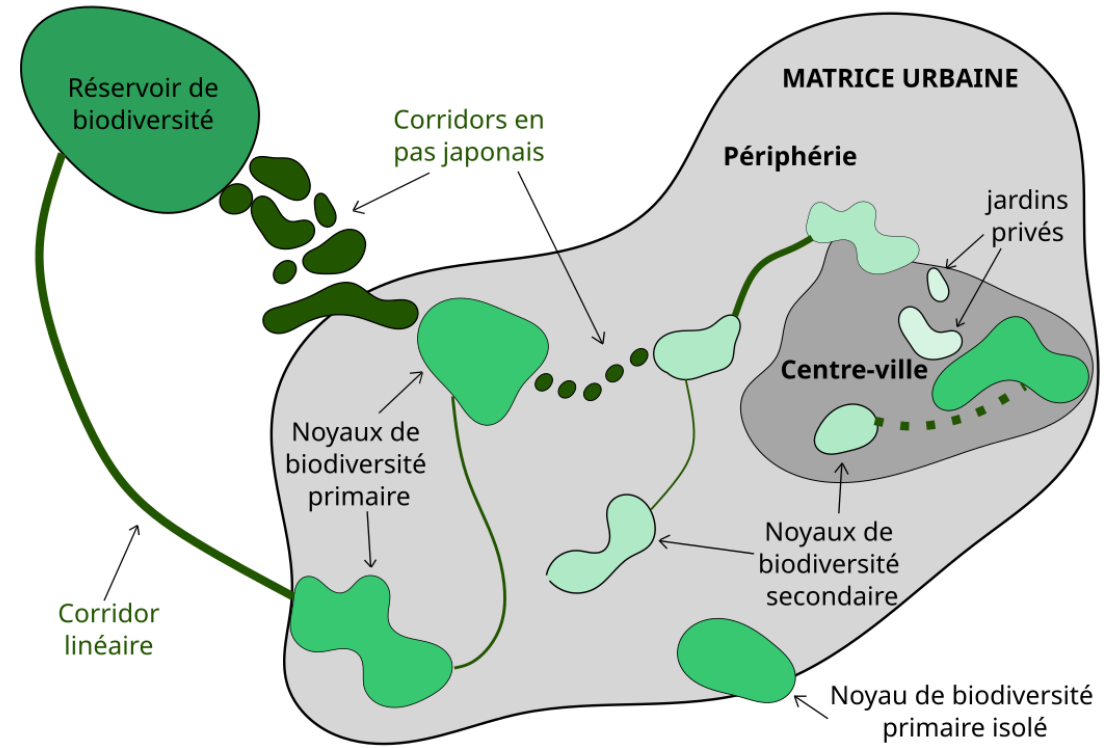
\includegraphics[width=0.78\textwidth]{figures/tvburbaine_schema.png}
\caption{Schéma théorique d'une trame verte urbaine : réservoir, noyaux de biodiversité primaires et secondaires, corridors linéaires et en pas japonais, de la périphérie au centre-ville (©Cerema, 2023, d'après Clergeau \& Blanc, 2013).}
\label{fig:reseau}
\end{figure}

\section{Des engagements internationaux aux documents d'urbanisme}
La connectivité urbaine figure nommément dans les engagements internationaux les plus récents. La cible 12 du Cadre mondial de la biodiversité de Kunming-Montréal, adopté en 2022 par les parties à la Convention sur la diversité biologique, appelle à accroître la superficie, la qualité et la connectivité des espaces verts et bleus en zones urbaines.

À l'échelle européenne, la Stratégie en faveur de la biodiversité à l'horizon 2030 fixe des objectifs contraignants, dont la protection de 30 \% des terres et des mers de l'Union (Commission européenne, 2020). Le règlement (UE) 2024/1991 sur la restauration de la nature va plus loin en imposant aux États une absence de perte nette d'espaces verts urbains, ainsi que la remise d'un plan national de restauration dont l'échéance est fixée au 1er septembre 2026. La déclinaison française dédiée aux milieux urbains relève pour sa part du plan national Nature en ville 2024-2030.

En France, la préservation de ces continuités est devenue une obligation de prise en compte dans la planification. La Trame verte et bleue, instituée par les lois Grenelle I (2009) et II (2010), s'est déclinée en schémas régionaux de cohérence écologique (SRCE), intégrés depuis 2016 aux schémas régionaux d'aménagement, de développement durable et d'égalité des territoires (SRADDET). Les documents d'urbanisme, du schéma de cohérence territoriale (SCoT) au plan local d'urbanisme (PLU, PLUi), doivent prendre en compte ces continuités (article L. 371-3 du code de l'environnement).

Ce cadre s'assouplit au fur et à mesure en descendant vers le territoire où se décident les aménagements. Les cibles du règlement européen s'imposent aux États, mais elles n'ont pas encore été transposées en obligations pesant sur les documents d'urbanisme, où les continuités relèvent de la seule prise en compte. Aucun résultat mesurable ne s'impose donc à une collectivité sur ce point. Ainsi, face à des budgets contraints, elles privilégient leurs missions obligatoires, et le diagnostic de continuités écologiques passe alors au second plan. Un outil peu coûteux à produire et lisible sans expertise préalable permettrait aux acteurs concernés de se saisir du sujet. Le travail présenté produit des continuités écologiques potentielles, c'est-à-dire un diagnostic modélisé destiné à éclairer une décision, et non une Trame verte et bleue réglementaire, dont l'identification suppose une concertation et une validation de terrain.

\section{Le projet UrbiVerde, cadre du stage}
Le stage s'est déroulé chez Murmuration, PME toulousaine fondée en mars 2019 par des ingénieurs issus du secteur spatial. L'entreprise s'est d'abord constituée autour de la mesure de l'impact environnemental de l'activité touristique, à destination des décideurs de ce secteur, avant d'élargir son domaine à l'aide à la décision environnementale pour les collectivités, les entreprises et les organisations publiques. Son activité consiste à dériver de l'observation satellitaire des indicateurs environnementaux, couvrant six principaux thèmes : air, biodiversité, climat, eau, sol et activités humaines. Ces indicateurs sont principalement diffusés sous forme de tableaux de bord.

L'effectif est de vingt et une personnes, organisées en une équipe commerciale, une équipe de conduite de projet et une équipe d'ingénierie. L'ingénierie est organisée selon les étapes de la vie d'un indicateur. La recherche et développement le conçoit et le prototype par le traitement de données géospatiales. L'architecture logicielle, l'infrastructure et le déploiement côté serveur l'industrialisent, c'est-à-dire le transforment en chaîne de traitement exploitable en production. Enfin, la visualisation le restitue dans les interfaces et les tableaux de bord livrés aux clients. J'ai intégré l'équipe recherche et développement, composée de cinq autres personnes, sous l'encadrement d'Hugo Poupard qui en est responsable.

Ce stage s'inscrit dans le projet UrbiVerde, soutenu par l'Agence Spatiale Européenne dans le cadre de son programme Information Factory Pathfinder for Adaptation, qui finance des infrastructures transformant les données d'observation de la Terre en information utile à l'adaptation au changement climatique. UrbiVerde vise à démontrer la faisabilité d'une plateforme en ligne d'aide à la décision, donnant accès à des indicateurs liés aux problématiques urbaines (îlots de chaleur, santé de la végétation, gestion de l'eau, pollution de l'air, pollution lumineuse et sonore, ...).

Quatre partenaires composent le consortium. CS Group assure l'intégration de la plateforme et le traitement des données, Murmuration le traitement de données d'observation de la Terre et le développement de services d'information environnementale, le Cerema l'expertise publique en aménagement durable et l'accès aux besoins des utilisateurs finaux, et Aerospace Valley l'accès au marché. L'ESA impose au projet deux exigences, réutiliser l'existant plutôt que recréer des outils, et viser une plateforme opérationnelle pérenne. Ce stage s'inscrit dans le service consacré aux continuités écologiques en milieu urbain.

\section{État de l'art}
\subsection{Sources et produits d'occupation du sol}
Pour modéliser la connectivité écologique, il est nécessaire de décrire le paysage et les habitats pertinents pour les espèces, notamment à l'aide de données d'occupation du sol. L'observation de la Terre présente pour cet usage trois avantages sur les inventaires de terrain. Elle couvre l'intégralité d'un territoire de façon homogène, elle se répète à intervalle régulier, et elle produit une donnée traitable par des procédures identiques d'un site à l'autre.

Deux voies existent pour obtenir ces données d'entrée. La première produit une classification sur mesure à partir d'images satellites. Elle repose sur un apprentissage supervisé : un algorithme apprend à reconnaître les classes sur des échantillons annotés par un opérateur, puis applique cette règle à l'ensemble de l'image. L'approche historique procède pixel à pixel, chaque cellule étant affectée à une classe d'après sa signature spectrale, ou d'après sa trajectoire temporelle lorsqu'une série d'images est disponible (Inglada et al., 2017). L'analyse orientée objet regroupe au préalable les pixels en segments homogènes avant de les classer, ce qui atténue l'effet poivre et sel, et permet de mobiliser la forme et le contexte des objets (Blaschke, 2010). La segmentation sémantique profonde en est le prolongement récent. Performante, elle est cependant coûteuse à transposer, car elle suppose une imagerie très haute résolution ou des données annotées. Toute classification supervisée est en outre exposée au glissement de domaine, les échantillons d'apprentissage issus d'une région ne valant pas pour une autre sans ré-entraînement (Tuia et al., 2016).

La seconde voie réutilise des produits prêts à l'emploi. Les produits nationaux sont fins, qu'ils proviennent d'une classification supervisée de séries temporelles (Inglada et al., 2017) ou de la photo-interprétation de référentiels comme l'OCS GE, la CoSIA ou la BD TOPO, mais sont restreints à un pays et donc incompatibles avec une chaîne de traitement couvrant plusieurs pays. Les produits mondiaux sont disponibles partout, au prix d'une résolution de 10 m inférieure à la taille de nombreux éléments du réseau écologique urbain (Radoux et al., 2016). Leur précision, de 73 \% à 84 \% pour les principaux d'entre eux, se dégrade dans les paysages hétérogènes comme le tissu urbain (Xu et al., 2024). Les résolutions fines s'obtiennent ainsi presque toujours au prix de l'étendue, en mobilisant des données nationales ou locales, tandis que les travaux menés à l'échelle continentale se limitent parfois à 30 m avec un petit nombre de classes, la carte servant alors à évaluer la perméabilité générale d'une région plutôt que les déplacements internes à la ville (Pundsack et al., 2025).

OpenStreetMap comble une part du manque laissé par les produits mondiaux, en apportant les objets qui en sont absents ou trop grossiers. Sa complétude routière mondiale était estimée à plus de 80 \% en 2016 (Barrington-Leigh \& Millard-Ball, 2017).

Aucune source ne réunit donc finesse, couverture mondiale, gratuité et reproductibilité.

\subsection{Modéliser la connectivité : de l'habitat au réseau}
Une fois l'occupation du sol acquise, la modélisation procède en trois étapes : identifier où se situe l'habitat, évaluer la résistance qu'oppose le reste du paysage au déplacement, puis en déduire le réseau qui en résulte. Chacune dispose de méthodes établies et repose sur des choix de paramétrage dont la littérature documente le poids.

Premièrement, pour délimiter l'habitat, la carte d'occupation du sol est transformée en une couche binaire, habitat ou non-habitat, selon les milieux que l'espèce considérée peut occuper. L'analyse morphologique des motifs spatiaux (MSPA), introduite par Vogt et al. (2007), applique à cette couche des opérations de morphologie mathématique. Une érosion retire une bande de largeur fixée au pourtour de chaque tache, une dilatation la restitue ensuite, et chaque pixel d'habitat se trouve classé selon sa géométrie, cœur intérieur, îlot, lisière... La méthode sépare ainsi les taches dotées d'un cœur, candidates au rôle de réservoir, des petits éléments qui peuvent servir de relais. Sa principale limite tient à ce que la largeur de bord n'a pas de valeur de référence. Les sorties dépendent de ce paramètre, de la résolution et de la règle de binarisation retenus (Ostapowicz et al., 2008), que les logiciels de référence documentent comme des choix d'utilisateur (Vogt \& Riitters, 2017).

Le déplacement hors de l'habitat est représenté par une surface de résistance, fondement commun de la plupart des modèles de connectivité (Diniz et al., 2020). Il s'agit d'un raster où chaque cellule reçoit un coût de franchissement traduisant la difficulté qu'un organisme rencontre à la traverser, du fait de l'effort physiologique ou du risque de mortalité associés au milieu (Adriaensen et al., 2003 ; Spear et al., 2010). Cette représentation fait passer les modèles d'un paysage homogène, où seule compte la distance, à des paysages différenciés où la nature des milieux traversés compte autant que leur étendue. Construire une telle surface suppose de choisir les variables environnementales susceptibles d'affecter le déplacement, réunir des données de mouvement (détections, relocalisations, trajets suivis, données génétiques) puis de relier statistiquement les deux pour en déduire des valeurs de coût (Diniz et al., 2020). Ces données de terrain faisant souvent défaut, les valeurs sont majoritairement fixées à dire d'expert et rarement calibrées empiriquement (Zeller et al., 2012), d'où des recommandations divergentes d'une étude à l'autre pour une même espèce (Beier et al., 2008).

Sur cette surface de résistance s'appuient trois familles de modèles de déplacement (Figure~\ref{fig:diniz}a). La méthode des chemins de moindre coût (Figure~\ref{fig:diniz}b) identifie le trajet qui minimise le coût cumulé entre deux taches, c'est-à-dire la somme des coûts des cellules traversées (Adriaensen et al., 2003). Cette famille a été validée expérimentalement en milieu urbain (Balbi et al., 2019). Le tracé produit est toutefois un trait de largeur nulle, et le chemin optimal en coût ne désigne pas l'emprise d'un corridor à aménager (Pinto \& Keitt, 2009 ; Etherington, 2016). Sa fiabilité dépend en outre des valeurs de résistance rarement confrontées au mouvement réel (Sawyer et al., 2011).

La théorie des circuits (Figure~\ref{fig:diniz}c) assimile le paysage à un réseau électrique où le courant emprunte simultanément tous les trajets possibles. Elle restitue un gradient de perméabilité plutôt qu'une ligne unique et met en évidence les points de passage obligatoires (McRae et al., 2008 ; Koen et al., 2014). Une troisième famille, les modèles individus-centrés (Figure~\ref{fig:diniz}d), simule des agents dotés de règles de déplacement, au prix d'exigences en données nettement supérieures.

\begin{figure}[H]
\centering
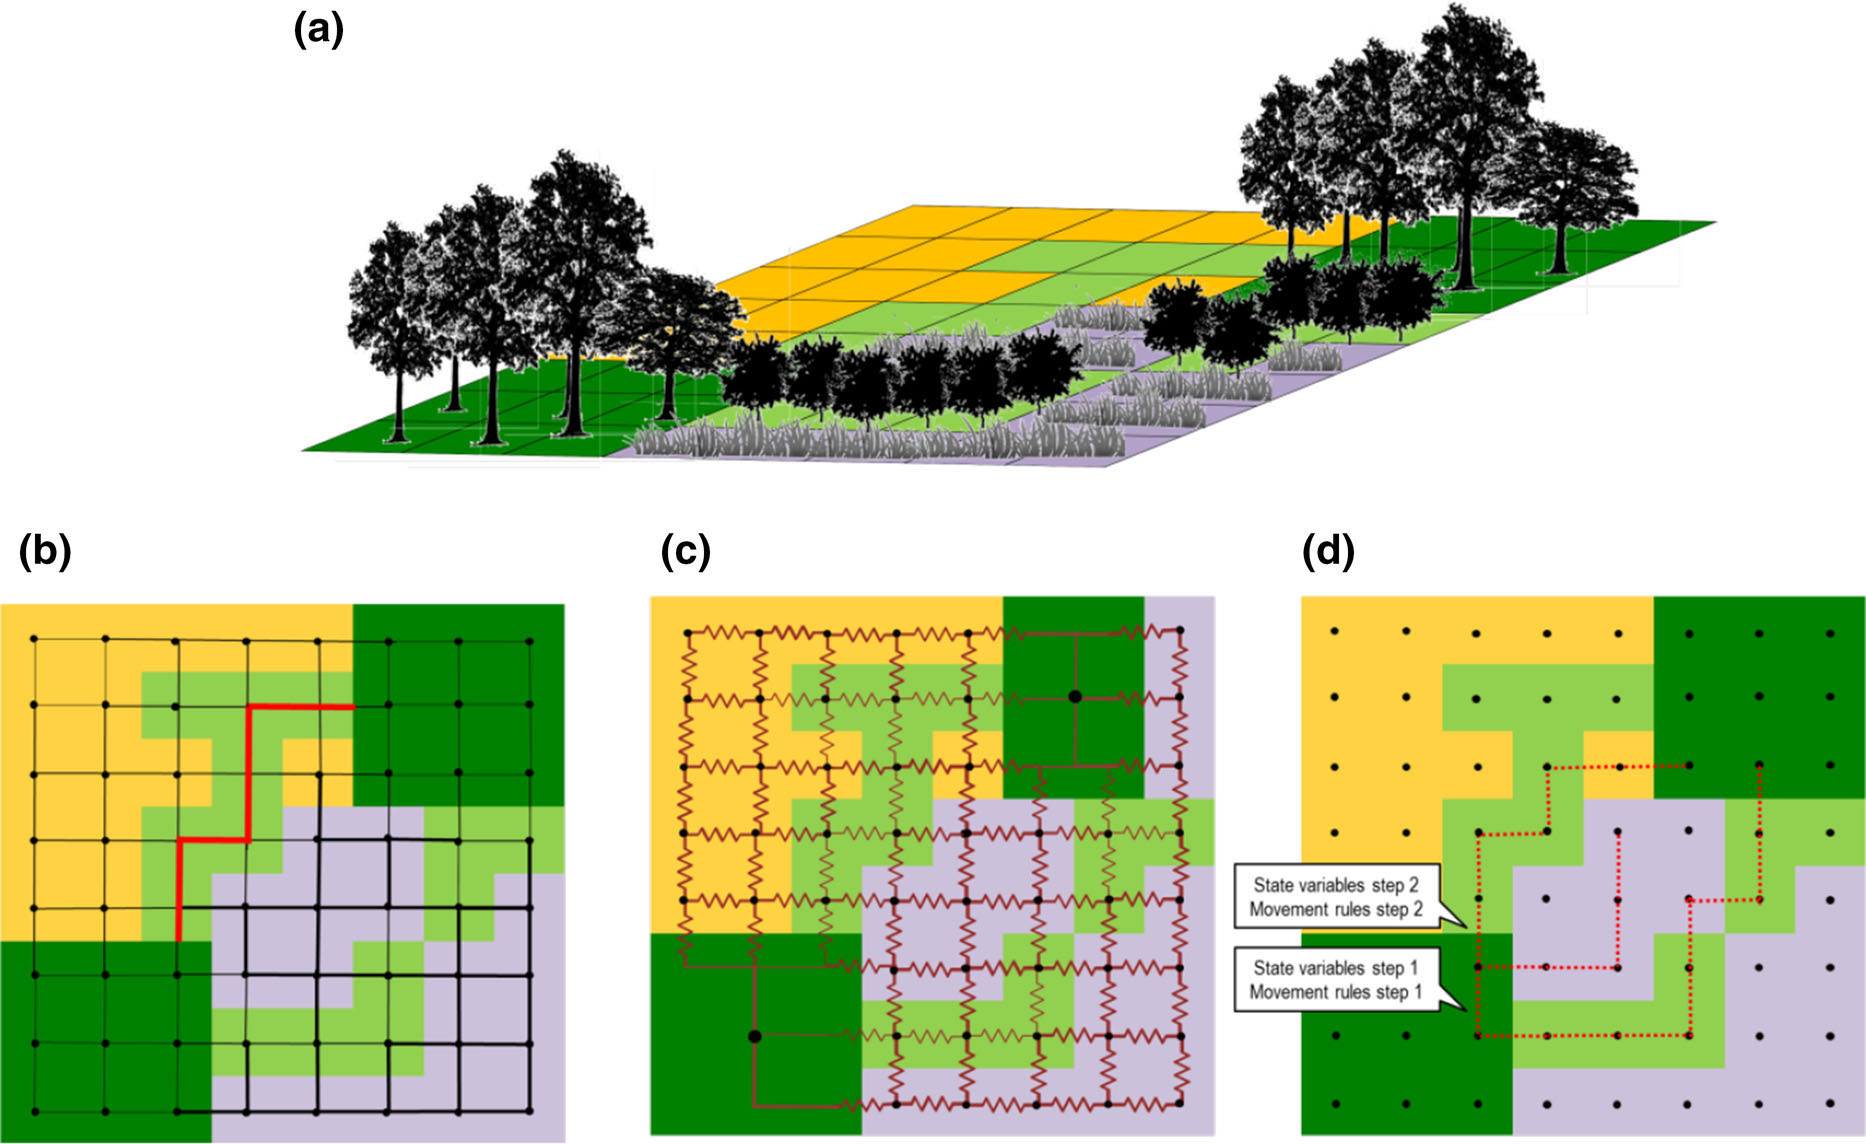
\includegraphics[width=\textwidth]{figures/diniz_connectivity_models.png}
\caption{Surface de résistance au déplacement (a) et familles de modèles associées : moindre coût (b), théorie des circuits (c), modèle individu-centré (d). Les couleurs représentent des classes d'occupation du sol associées à des niveaux de friction croissants (d'après Diniz et al., 2020).}
\label{fig:diniz}
\end{figure}

Pour obtenir le réseau écologique, le paysage est représenté par un graphe paysager dont les taches d'habitat sont les nœuds et les connexions possibles les liens (Urban \& Keitt, 2001 ; Fall et al., 2007). Chaque lien est pondéré par une probabilité de déplacement qui décroît exponentiellement avec la distance séparant les deux taches, à un rythme réglé par la distance caractéristique de dispersion de l'espèce. Cette distance peut être mesurée en ligne droite. Elle peut aussi être remplacée par le coût cumulé du chemin de moindre coût, auquel cas le graphe hérite de la surface de résistance et représente une connectivité fonctionnelle et non plus seulement géométrique. La topologie du graphe constitue un troisième choix de modélisation. Le nombre de paires de taches reliées, du graphe le plus parcimonieux aux plus denses, modifie sensiblement le diagnostic de connectivité, sans qu'un consensus se dégage sur la variante à retenir (Minor \& Urban, 2008 ; Galpern et al., 2011).

De cette représentation dérivent les indices de disponibilité d'habitat, qui mesurent la quantité d'habitat atteignable en traitant chaque tache à la fois comme une surface et comme un relais vers les autres (Saura \& Pascual-Hortal, 2007). L'Integral Index of Connectivity en est la version binaire, deux taches étant connectées ou non (Pascual-Hortal \& Saura, 2006). La Probability of Connectivity le généralise par la probabilité continue de déplacement, et s'interprète comme la probabilité que deux points tirés au hasard dans le paysage tombent dans des habitats mutuellement accessibles. Elle se traduit en surface équivalente connectée, qui exprime la même information en unité de surface, à savoir la taille qu'aurait un bloc d'habitat unique et parfaitement connecté (Saura et al., 2011).

Aucune de ces méthodes n'est universelle. Le choix dépend de l'objectif et de l'échelle d'analyse, les approches structurelles, fonctionnelles et de réseau éclairant des facettes différentes de la connectivité, et la comparaison de quatre d'entre elles sur un même paysage périurbain montre que les résultats varient selon l'objectif de conservation retenu (Pechanec et al., 2025). Trois limites traversent en revanche l'ensemble : des paramètres fixés à dire d'expert et rarement calibrés, une forte sensibilité des sorties à ce paramétrage, et une confrontation au mouvement réel qui reste l'exception.

\subsection{Représenter la faune : des sous-trames aux profils écologiques}
Paramétrer un modèle de connectivité par espèce suppose des données de distribution et de mouvement souvent indisponibles en ville. Les bases d'occurrence comme le GBIF (Global Biodiversity Information Facility) reposent largement sur des observations opportunistes issues des sciences participatives. L'effort d'observation y est inégal, concentré sur les zones accessibles et les espèces les plus visibles, au détriment des taxons discrets ou nocturnes et des secteurs peu fréquentés. La donnée reflète alors autant la répartition des observateurs que celle des espèces (Boakes et al., 2010 ; Isaac et al., 2014). Les données empiriques de déplacement sont plus rares encore (Kirk et al., 2023), un modèle qui en dépendrait ne serait ni transposable ni pérenne. Représenter la faune impose alors de choisir un niveau d'abstraction. Deux types d'entrées coexistent, les milieux, qui structurent la planification française, et les espèces, qui sont privilégiées dans la littérature internationale.

L'entrée par les milieux est celle de la Trame verte et bleue. Une sous-trame désigne l'ensemble des espaces d'un même type de milieu et le réseau qu'ils forment. La notion est définie par le décret du 27 décembre 2012 et précisée par les orientations nationales, qui fixent cinq sous-trames auxquelles chaque élément de trame doit être rattaché pour assurer la cohérence entre territoires (Sordello et al., 2017). À chaque sous-trame peut correspondre un cortège d'espèces, c'est-à-dire un ensemble d'espèces inféodées à ce type de milieu, aux exigences écologiques proches et susceptibles d'y coexister. Cette approche est lisible pour la planification, puisque les documents d'urbanisme raisonnent déjà par milieux, et elle se cartographie directement depuis l'occupation du sol. Cependant, elle présuppose que les espèces d'une même sous-trame partagent les mêmes besoins de déplacement, ce que contredisent les réponses contrastées à la fragmentation observées entre groupes de dispersion au sein d'un même milieu (Lechner et al., 2017). La friction moyenne d'un cortège lisse par ailleurs les écarts entre ses espèces les moins et les plus mobiles. Enfin, distinguer les sous-trames exige une occupation du sol séparant les strates de végétation, une finesse que les produits disponibles offrent rarement.

L'entrée par les espèces se décline en une série d'approches, du plus simple en données au plus exigeant. La plus basique est l'espèce substitut unique, dont les exigences dimensionnent le réseau (Lambeck, 1997), et à laquelle un rôle d'espèce parapluie est parfois prêté, même si un substitut unique ne représente souvent pas mieux les autres espèces qu'une espèce tirée au hasard (Andelman \& Fagan, 2000).

Pour pallier les limites d'un substitut unique, deux voies multi-espèces existent. La première retient plusieurs espèces focales complémentaires, aux exigences contrastées. Sur quatorze espèces de vertébrés du périurbain de Montréal, Albert et al. (2017) montrent qu'intégrer ainsi la connectivité de plusieurs espèces modifie sensiblement les priorités de conservation. La seconde abandonne les espèces réelles au profit d'espèces génériques ou chimères, un groupe d'espèces partageant les mêmes exigences d'habitat et la même capacité de déplacement y est représentée par une espèce fictive unique. Introduite avec les indices de paysage mis à l'échelle de l'écologie des espèces (Vos et al., 2001), la notion a été formalisée par Opdam et al. (2008) dans un cadre de planification territoriale participative, avec un objectif qui rejoint celui du présent travail, rendre une connaissance écologique utilisable par des acteurs qui ne sont pas écologues. Les auteurs rapportent que la méthode a bien été comprise par les décideurs des deux territoires d'application.

Le niveau de représentation choisi n'est pas neutre pour la décision, une évaluation multi-taxons pouvant modifier un arbitrage d'aménagement (Gelmi-Candusso et al., 2025). Les deux entrées ne s'excluent d'ailleurs pas, un profil pouvant être rattaché à la sous-trame dont il fréquente les milieux, mais elles n'exigent pas les mêmes données. L'entrée par les milieux demande une occupation du sol fine, quand un profil générique se paramètre à partir de traits documentés dans la littérature. Chacune établit un compromis différent entre exigence en données et réalisme écologique, et le choix dépend des données disponibles et de l'objectif (Tälle et al., 2023).

\subsection{Outils existants et verrou opérationnel}
Plusieurs logiciels mettent en œuvre les méthodes décrites pour modéliser la connectivité écologique. Graphab traite les graphes paysagers (Foltête et al., 2012), Conefor les indices de connectivité (Saura \& Torné, 2009), Circuitscape la théorie des circuits (McRae et al., 2008), et des extensions QGIS comme Biodispersal ou MitiConnect enchaînent ces étapes, la seconde autour de la séquence Éviter-Réduire-Compenser. La démarche de Kirk et al. (2023) procède également par un enchaînement manuel d'opérations sous QGIS, complété par un tableur pour le calcul des indicateurs.

Ces outils limitent pourtant leur usage opérationnel à grande échelle. Ils requièrent une expertise en système d'information géographique et une préparation manuelle des couches, sont le plus souvent appliqués au cas par cas sur des données fines locales, et restituent rarement des résultats directement exploitables par un gestionnaire non spécialiste. Trois travaux publiés illustrent l'état de l'assemblage de toutes ces méthodes, chacun couvrant une part de ce qui est recherché ici. Pundsack et al. (2025) traitent l'occupation du sol, avec la même exigence de reproductibilité, en fournissant une chaîne de production de carte fine réplicable d'une ville à l'autre, mais leur démarche s'arrête à cette donnée d'entrée, sur l'emprise européenne. Liu et al. (2022) enchaînent la chaîne complète sur Pékin, de l'analyse morphologique aux métriques de graphe puis au moindre coût et à la théorie des circuits, mais à l'échelle régionale, sans différencier les espèces, et par assemblage manuel de logiciels de bureau. Kirk et al. (2023) opèrent à l'intérieur de la ville, par groupes d'espèces et de façon reproductible autour de scénarios avant et après aménagement, mais avec une connectivité binaire et un enchaînement d'opérations qui reste manuel. Les travaux portant sur plusieurs villes restent l'exception.

Chacun des enjeux abordés, cet état de l'art dégage une réponse, mais toujours au prix d'un compromis. Une seule voie de données est à la fois libre et transposable partout, au prix de la résolution. Les méthodes de modélisation sont établies, mais paramétrées à dire d'expert et rarement confrontées au mouvement réel. Les manières de représenter le vivant sont documentées, mais il n'y a pas de consensus sur celle à adopter. Et les outils qui les mettent en œuvre demandent une expertise en système d'information géographique, s'appliquent au cas par cas et restituent des résultats que les gestionnaires n'exploitent pas directement. Une chaîne qui serait automatisée, fondée sur des données ouvertes, applicable sans réglage local à des territoires contrastés et dont les sorties seraient utilisables par un non-spécialiste n'existe pas dans la littérature examinée. C'est cette combinaison que le présent travail cherche à construire.

\section{Problématique et objectifs}
Ce stage a consisté à proposer une preuve de concept : une chaîne de traitement qui identifie les continuités écologiques urbaines potentielles à partir de l'observation de la Terre et de données ouvertes.

De ce positionnement découle la problématique du stage :

\textit{Comment construire un outil de connectivité écologique urbaine, piloté par l'observation de la Terre et des données ouvertes, reproductible sur des territoires aux contextes bioclimatiques contrastés, et produisant des résultats spatialisés exploitables par les acteurs de l'améngement urbain ?}

Cette question se décline en cinq objectifs.

\begin{enumerate}
\item Concevoir une chaîne de traitement complète, depuis les données ouvertes jusqu'aux composantes des continuités écologiques potentielles.
\item Produire un diagnostic différencié selon les exigences écologiques des espèces, en représentant plusieurs profils plutôt qu'une espèce unique, et sans recalibrage propre à chaque territoire.
\item Implémenter l'ensemble en Python, sans recourir aux logiciels spécialisés existants, pour obtenir une chaîne automatisable, reproductible et transposable.
\item Restituer les résultats dans un tableau de bord d'aide à la décision destiné aux aménageurs.
\item Tester la transposabilité et la fiabilité de la chaîne sur des contextes bioclimatiques et urbains contrastés.
\end{enumerate}
La portée attendue de l'outil mérite d'être délimitée avant d'exposer la méthode. La chaîne produit un pré-diagnostic comparatif de connectivité potentielle. Il ne se substitue ni à une étude écologique locale, ni à l'expertise d'un écologue, ni à l'identification d'une trame verte et bleue réglementaire. Il intervient en amont de ces démarches, pour sensibiliser aux enjeux de continuité, comparer des territoires et des profils écologiques entre eux, hiérarchiser les secteurs où une étude fine se justifie, et estimer l'effet attendu d'un projet d'aménagement avant sa réalisation. Cette position en amont est cohérente avec la vocation d'aide à la décision assignée au service dans le projet UrbiVerde, et avec le constat que l'adoption des travaux de connectivité par la planification dépend d'abord de leur transparence et de leur reproductibilité (Keeley et al., 2019).

\chapter{Données et méthodes}
\section{Territoires d'étude}
La méthode a été appliquée à des territoires aux contextes bioclimatiques contrastés (Figure~\ref{fig:localisation}). Les quatre villes pilotes du projet UrbiVerde ont constitué le socle du développement : La Roche-sur-Yon, Nancy, Perpignan et Kourou. Deux territoires supplémentaires ont été ajoutés. Toulouse a été retenue comme cas de contrôle visuel, en raison d'une bonne connaissance du terrain. L'agglomération de La Rochelle a été ajoutée car c'est le territoire de la méthode Cerema Dter Sud-Ouest (2025) à laquelle ce travail se réfère plusieurs fois.

\begin{figure}[H]
\centering
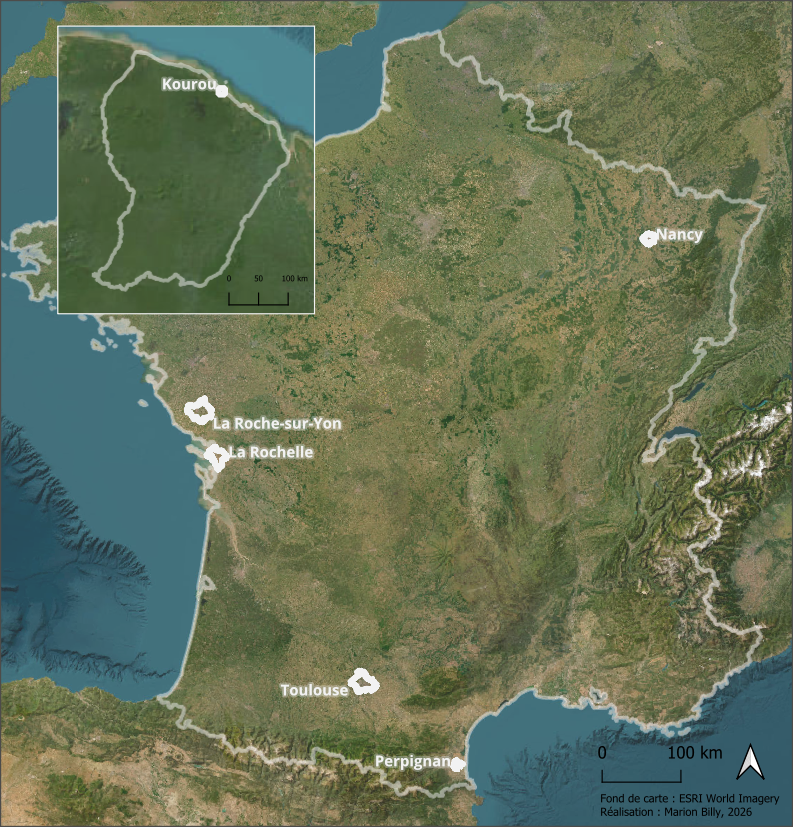
\includegraphics[width=0.90\textwidth]{figures/aoi_loc.png}
\caption{Localisation des six territoires d'étude, emprises des zones d'étude et encart sur la Guyane.}
\label{fig:localisation}
\end{figure}

Pour chaque territoire, la zone d'étude est définie à partir de ses limites administratives ; Kourou fait exception, avec une emprise rectangulaire, sa limite communale étant trop restreinte pour englober les espaces périurbains pertinents. Ce choix se justifie par la destination du diagnostic, une collectivité étant responsable d'un périmètre administratif. Cette zone est ensuite élargie par un tampon égal à deux fois la plus grande distance de dispersion considérée, soit six kilomètres. Ce tampon corrige l'effet de bord, une frontière de carte artificielle se comportant comme une barrière qui sous-estime la connectivité des taches périphériques (Koen et al., 2010, 2014). Un corridor peut en effet s'appuyer sur une tache d'habitat située juste en dehors de la limite administrative, qui serait ignorée si l'analyse s'arrêtait à cette limite. Les habitats du tampon servent ainsi de relais au calcul, mais seules les composantes situées dans la zone d'étude stricte sont comptabilisées dans les résultats. Les analyses sont menées dans la projection métrique locale de chaque territoire.

La superficie de la zone d'étude varie fortement d'un territoire à l'autre, de 68 km² à Perpignan à 502 km² à La Roche-sur-Yon (Table~1). Cette différence doit être considérée pour lire les surfaces d'habitat et la surface connectée équivalente, qui croissent mécaniquement avec l'étendue du territoire. La part d'habitat connecté, exprimée en pourcentage, est en revanche construite pour rester comparable entre des emprises de tailles différentes.

\begin{table}[H]
\centering
\caption{Les six territoires d'étude, leur statut, leur contexte bioclimatique et la superficie de la zone d'étude.}
\begin{tabularx}{\textwidth}{>{\raggedright\arraybackslash}X >{\raggedright\arraybackslash}X >{\raggedright\arraybackslash}X >{\raggedright\arraybackslash}X}
\toprule
\textbf{Territoire} & \textbf{Statut} & \textbf{Contexte bioclimatique} & \textbf{Zone d'étude (km², tampon inclus)} \\
\midrule
La Roche-sur-Yon & pilote & atlantique & 502 \\
Nancy & pilote & continental (nord-est) & 143 \\
Perpignan & pilote & méditerranéen & 68 \\
Kourou (Guyane) & pilote & équatorial & 123 \\
Toulouse & contrôle visuel & océanique à influence méditerranéenne & 461 \\
La Rochelle & référence (méthode Cerema) & atlantique & 331 \\
\bottomrule
\end{tabularx}
\end{table}

Kourou occupe un statut à part. Les profils écologiques, calibrés sur des espèces de métropole, n'y représentent pas la faune locale. Ce territoire sert donc de test de transposabilité à un biome très différent, non de diagnostic exploitable.

\section{Données et construction de l'occupation du sol enrichie}
La chaîne de traitement part d'une couche d'occupation du sol, d'où sont dérivés l'habitat propre à chaque profil écologique et la résistance de la matrice au déplacement. Elle repose sur le produit mondial ESA WorldCover v200 d'une résolution de dix mètres (Zanaga et al., 2022). Les données sont dérivées des imageries Sentinel-1 et Sentinel-2 et récupérées via Google Earth Engine sur l'emprise tamponnée. Les sources mobilisées, leur rôle dans la chaîne et leurs conditions d'accès sont récapitulés en annexe 1. Cette version, la plus récente du produit, est créditée d'une précision globale de 76,7 \% sur ses onze classes, et se situe au premier rang des produits mondiaux à dix mètres selon une évaluation externe indépendante (Zhao et al., 2023).

Ce produit ne représente toutefois pas avec la finesse requise les infrastructures fragmentantes, c'est-à-dire les aménagements linéaires que la faune terrestre ne franchit qu'au prix d'un détour ou d'un risque de mortalité. Routes, voies ferrées, emprises bâties et surfaces en eau sont donc ajoutées à partir d'OpenStreetMap, dont la complétude est la meilleure dans les villes denses (Barrington-Leigh \& Millard-Ball, 2017). Ces éléments sont rastérisés puis superposés au WorldCover selon un ordre de priorité détaillé en annexe 2. L'opération ajoute cinq codes d'occupation artificialisée, bâti (51), routes principales (52), routes secondaires (53), chemins (54) et voies ferrées (55). Le résultat est illustré Figure~\ref{fig:landcover} pour Toulouse. De plus, une correction de qualité est appliquée : WorldCover classe en prairie la pelouse rase des aérodromes et des stades, que les profils de milieux ouverts compteraient à tort comme habitat. Ces emprises, repérées par leurs attributs OpenStreetMap, sont donc gravées en surface imperméable.

Ce complément tient à la conception même de WorldCover, plus qu'à sa qualité de classement. Chaque pixel de dix mètres y est classé indépendamment, selon sa couverture dominante, sans logique d'objet qui permettrait de reconnaître un élément linéaire continu comme une route. Une voirie de moins de dix mètres de large, mélangée à ses abords dans le pixel qu'elle traverse, y est ainsi rarement identifiée comme telle. De même, l'unique classe «~built-up~» ne distingue pas une autoroute d'un lotissement. Les infrastructures fragmentantes sont donc absentes par construction, et non par erreur de classement.

La démarche a déjà été employée ailleurs. Gelmi-Candusso et al. (2024) partent du même constat, la matrice urbaine réduite à une classe bâtie homogène dans les cartes mondiales, et construisent une couche enrichie selon le même procédé : tampon des entités linéaires selon leur type, rastérisation, puis superposition selon une hiérarchie de priorité où les infrastructures l'emportent sur l'usage du sol.
% [À VÉRIFIER] la version publiée dans Ecology and Evolution (accès libre) donne des chiffres de qualité qui renforceraient ce paragraphe : coefficient kappa de la couche enrichie, part de la surface classée en routes sans type renseigné, et comparaison de la surface bâtie estimée aux emprises LiDAR locales. Ils proviennent du préprint bioRxiv 2023 et l'article publié compte trois auteurs de plus : les relever sur la version définitive avant de les citer.

\begin{figure}[H]
\centering
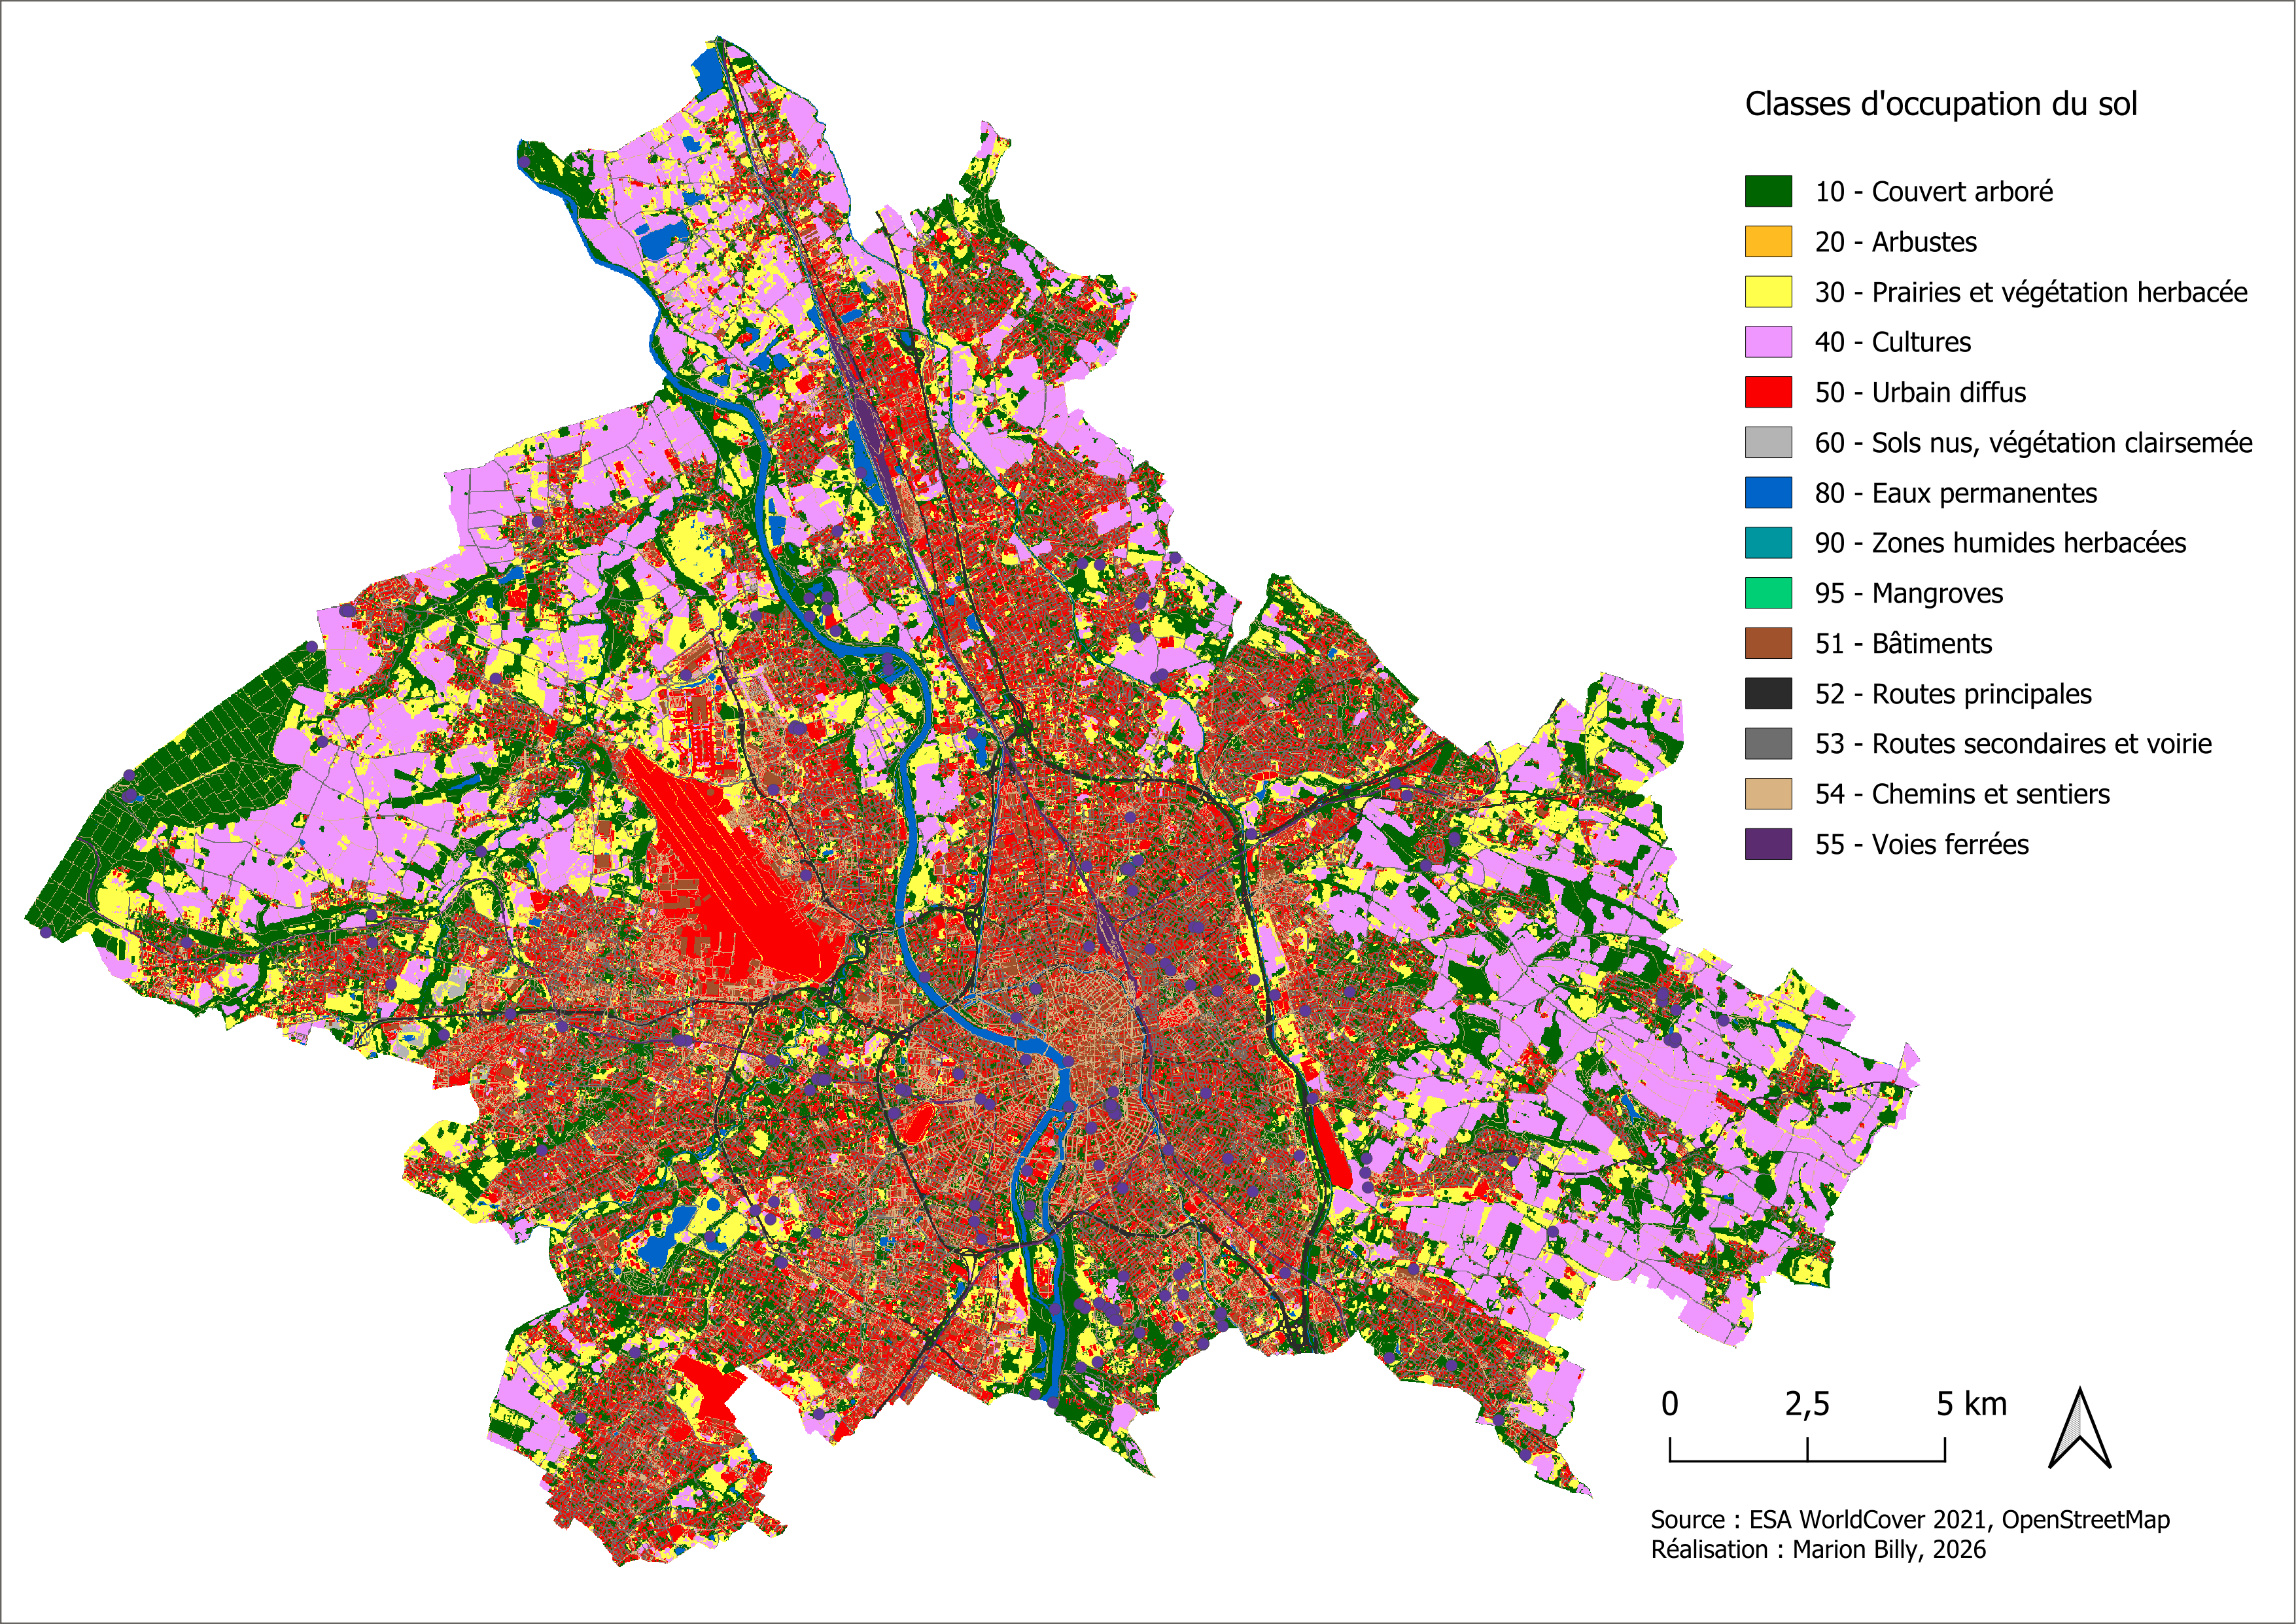
\includegraphics[width=\textwidth]{figures/landcover_toulouse.png}
\caption{Occupation du sol enrichie de Toulouse.}
\label{fig:landcover}
\end{figure}

La nomenclature obtenue satisfait les exigences que la littérature de connectivité urbaine formule pour une carte d'entrée, tant par sa résolution que par les classes qu'elle distingue (Pundsack et al., 2025).

Une donnée mondiale et gratuite garantit une chaîne identique d'un territoire à l'autre, et la continuité du diagnostic après la fin du financement du projet, là où une acquisition d'imagerie ville par ville représente un coût récurrent.

Cependant, les éléments les plus fins du réseau écologique urbain, haies étroites, alignements d'arbres, petites mares, sont plus petits que le pixel de dix mètres et entrainent une perte de détail (Radoux et al., 2016). Le service intégré au projet UrbiVerde prévoit une occupation du sol plus fine en entrée à terme, la couche étant conçue ici comme interchangeable au prix d'une adaptation de la nomenclature.

\section{Définition et calibration des profils écologiques}
Représenter la faune suppose de choisir un niveau d'abstraction et une source de paramètres, deux choix motivés ci-après : des profils écologiques multiples plutôt qu'une espèce unique, calibrés sur la littérature plutôt que sur des mesures locales.

Retenir plusieurs profils restitue une information qu'une entrée unique masque, les besoins de continuité variant fortement d'une espèce à l'autre (§1.5.3). Un profil écologique est défini ici par les classes d'occupation du sol qui constituent son habitat, sa distance caractéristique de dispersion et ses coefficients de friction par classe. Les quatre profils retenus se différencient par leur distance de dispersion et leurs classes d'habitat (Table~2), et portent le nom d'une espèce repère. Ce nom sert la lisibilité du profil pour des acteurs non-écologues, non à limiter la modélisation à cette seule espèce : il représente en réalité un ensemble d'espèces aux exigences comparables. Ces espèces ont été choisies parmi les communes de France métropolitaine, pour lesquelles la littérature documente à la fois l'habitat et la capacité de déplacement (Morris, 1988 ; Huijser \& Bergers, 2000 ; Avon et al., 2014 ; Quiblier, 2007). 

\begin{table}[H]
\centering
\caption{Caractéristiques des quatre profils écologiques (espèce repère, distance de dispersion, habitat, obstacles infranchissables) (d'après Cerema Dter Sud-Ouest, 2025).}
\begin{tabularx}{\textwidth}{>{\raggedright\arraybackslash}X >{\raggedright\arraybackslash}X >{\raggedright\arraybackslash}X >{\raggedright\arraybackslash}X >{\raggedright\arraybackslash}X}
\toprule
\textbf{Profil écologique} & \textbf{Espèce repère} & \textbf{d0 (m)} & \textbf{Habitat} & \textbf{Obstacles infranchissables} \\
\midrule
Mammifère terrestre & Hérisson d'Europe (\textit{Erinaceus europaeus}) & 3000 & arbres, arbustes, prairies & bâtiments, grandes rivières \\
Mammifère arboricole & Écureuil roux (\textit{Sciurus vulgaris}) & 2000 & arbres & bâtiments \\
Oiseau de lisière & Fauvette à tête noire (\textit{Sylvia atricapilla}) & 1500 & arbres, arbustes & aucune \\
Reptile de milieux ouverts & Lézard des murailles (\textit{Podarcis muralis}) & 750 & prairies, sols nus & bâtiments, grandes rivières \\
\bottomrule
\end{tabularx}
\end{table}

La calibration s'appuie sur trois sources principales. La méthode du Cerema Dter Sud-Ouest sur les continuités écologiques urbaines de l'agglomération de La Rochelle (2025) fournit la table de coefficients de friction et les distances de dispersion des espèces repères. C'est la référence principale, retenue parce qu'elle porte sur le milieu urbain, qu'elle est documentée classe par classe, et qu'elle est appliquée en France par un opérateur public. La littérature écologique sur les espèces repères est mobilisée pour vérifier la plausibilité des valeurs au regard des traits d'histoire de vie documentés. La littérature méthodologique sur les surfaces de résistance guide la construction des matrices de friction (Zeller et al., 2012 ; Beier et al., 2008).

Les coefficients de friction, sur une échelle de 1 pour un milieu optimal à 100 pour un obstacle, sont transposés de la nomenclature de la méthode duCerema Dter Sud-Ouest (2025), à la nomenclature plus agrégée de WorldCover enrichi. Chaque classe WorldCover regroupant plusieurs classes de la table d'origine, la valeur retenue est la moyenne des valeurs correspondantes. Une classe devient habitat du profil lorsque sa friction est inférieure ou égale à 3 (Cerema Dter Sud-Ouest, 2025). Les milieux réellement impénétrables reçoivent une résistance infinie, ce qui est le cas des bâtiments et des surfaces en eau selon les profils. Le détail figure en annexe 3. Ce qui structure le résultat est enfin moins le niveau de ces coefficients que le contraste entre classes, c'est-à-dire l'écart de résistance entre l'habitat et la matrice, les valeurs relatives déterminant la position des tracés de moindre coût plus que leur amplitude absolue (Rayfield et al., 2010). 

Les distances caractéristiques de dispersion sont reprises des fiches espèces (Cerema Dter Sud-Ouest, 2025), qui documentent la capacité de déplacement de chaque espèce repère à partir de la littérature naturaliste, guides de terrain, atlas régionaux et fiches d'organismes naturalistes.

\section{Chaîne de traitement}
Pour chaque couple territoire-profil écologique, la chaîne de traitement transforme le produit d'occupation du sol en un jeu de sorties complet, soit vingt-quatre jeux au total. Elle produit successivement les noyaux de biodiversité et les espaces relais, le graphe des connexions possibles entre eux, les tracés de moindre coût qui réalisent ces connexions, les surfaces de dispersion, et quatre indicateurs synthétiques. Les sous-sections suivent l'ordre d'exécution, et la Figure~\ref{fig:pipeline} en donne la vue d'ensemble. La première étape reprend la couche d'occupation du sol enrichie décrite en §2.2, découpée sur l'emprise élargie par le tampon.

\subsection{Habitat et segmentation morphologique}
Une couche d'habitat binaire est extraite en ne retenant que les classes d'habitat du profil écologique, puis segmentée par analyse morphologique (MSPA présentée en §1.5.2), avec une largeur de bord de dix mètres, soit un pixel, à l'aide d'un élément structurant carré de trois pixels de côté centré sur chaque pixel traité. Le classement qui en résulte repose sur deux critères distincts (Figure~\ref{fig:schema-mspa}). Une tache devient noyau de biodiversité lorsque son plus grand cœur compact, mesuré après érosion, atteint un hectare. La géométrie conservée en sortie est celle de la tache entière, lisière comprise, si bien que sa surface totale peut très largement excéder cet hectare. Une tache qui n'atteint pas ce seuil est classée en espace relais lorsqu'elle conserve un cœur compact, même réduit, et que sa surface totale atteint un dixième d'hectare. Les taches plus petites sont écartées, de même que les taches sans cœur, entièrement constituées de lisière (moins d'une trentaine de mètres de large en tout point) et donc dépourvues d'intérieur écologique : elles ne sont pas retenues comme points d'appui, quelle que soit leur surface.

\begin{figure}[H]
\centering
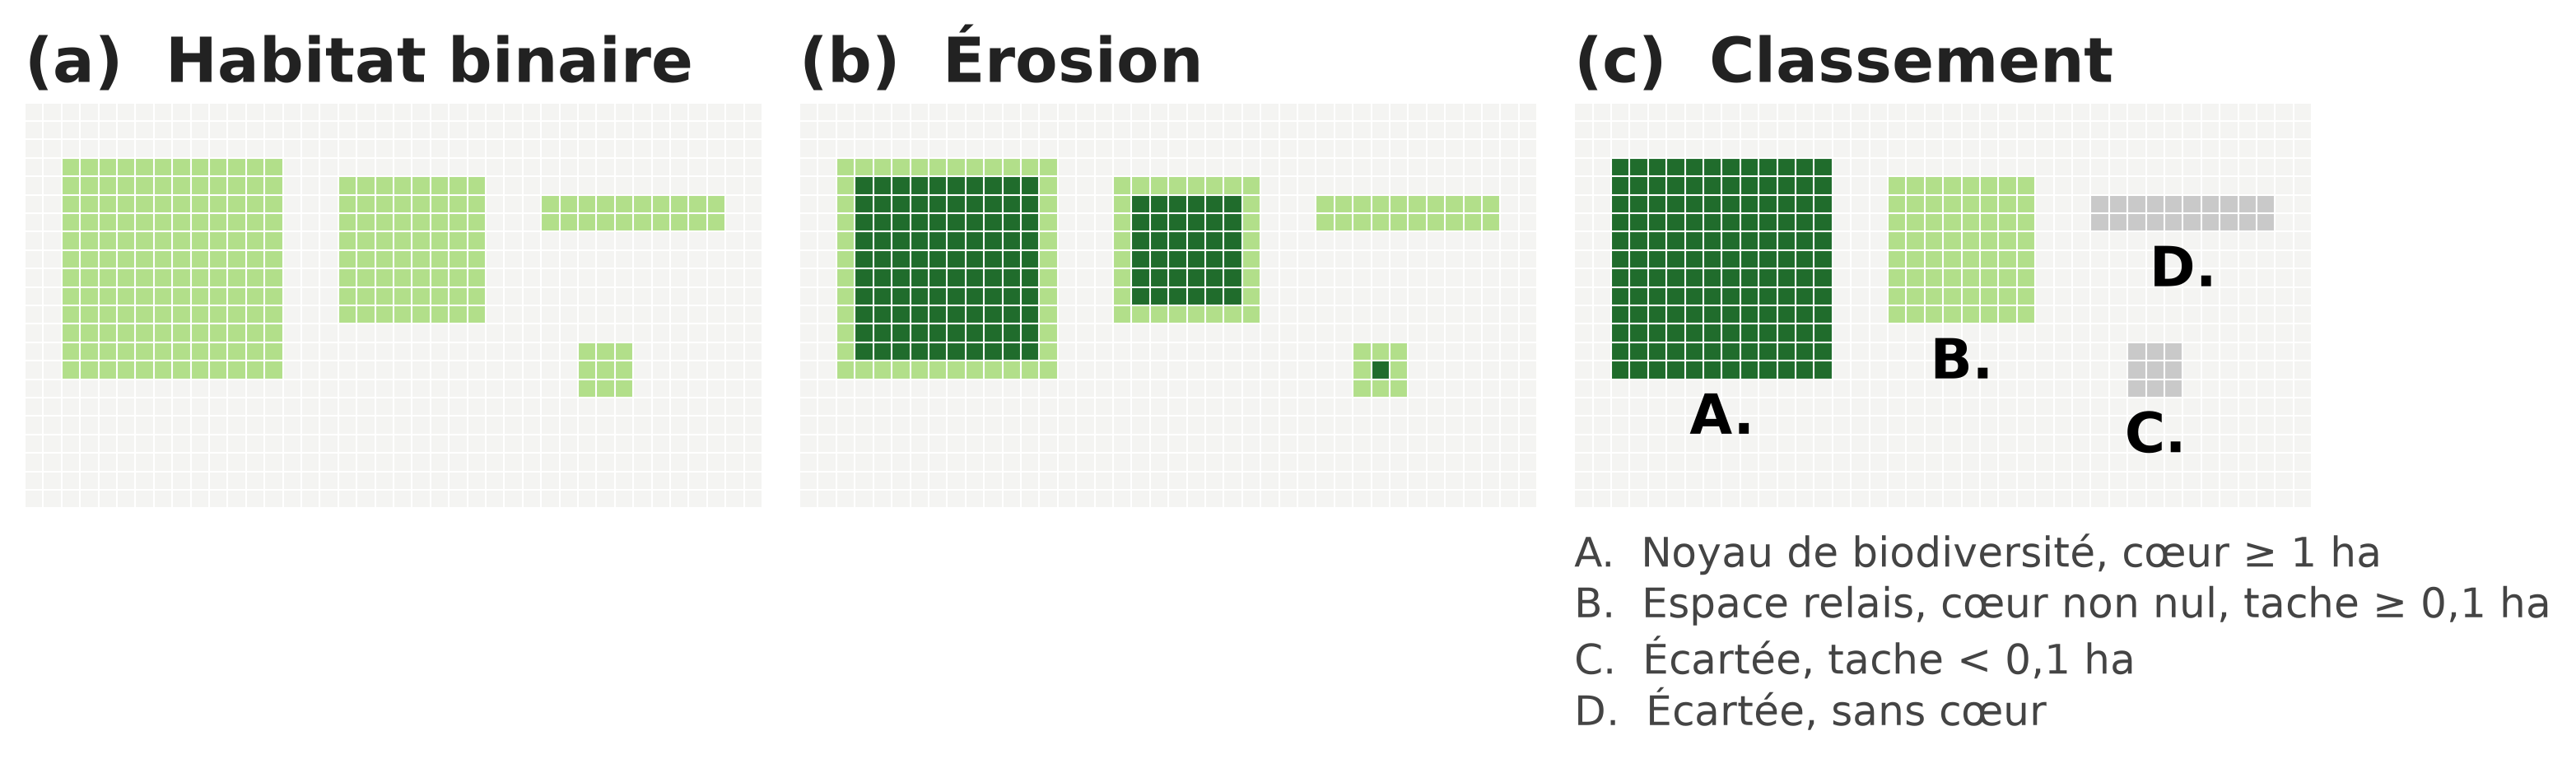
\includegraphics[width=\textwidth]{figures/schema_mspa.png}
\caption{Segmentation morphologique : (a) habitat binaire du profil ; (b) érosion d'un pixel (soit 10\,m), élément structurant de trois sur trois ; (c) classement et seuils appliqués. Réalisation personnelle, Python avec scipy.}
\label{fig:schema-mspa}
\end{figure}

La Figure~\ref{fig:mspa-perpignan} montre le résultat sur un secteur réel, la prairies des Filtres à Toulouse, pour le profil fauvette. De l'occupation du sol enrichie (a), la couche binaire (b) ne retient que les milieux arborés et arbustifs : une bande boisée continue le long de la Garonne. La segmentation morphologique appliquée (c) en tire les composantes du réseau : la prairie des Filtres devient un noyau de biodiversité, conservé avec sa lisière, et les fragments assez grands pour garder un cœur deviennent des espaces relais. La comparaison des panneaux (b) et (c) rend le tri visible : les petits fragments isolés de la couche binaire ont disparu, écartés par les seuils.

\begin{figure}[H]
\centering
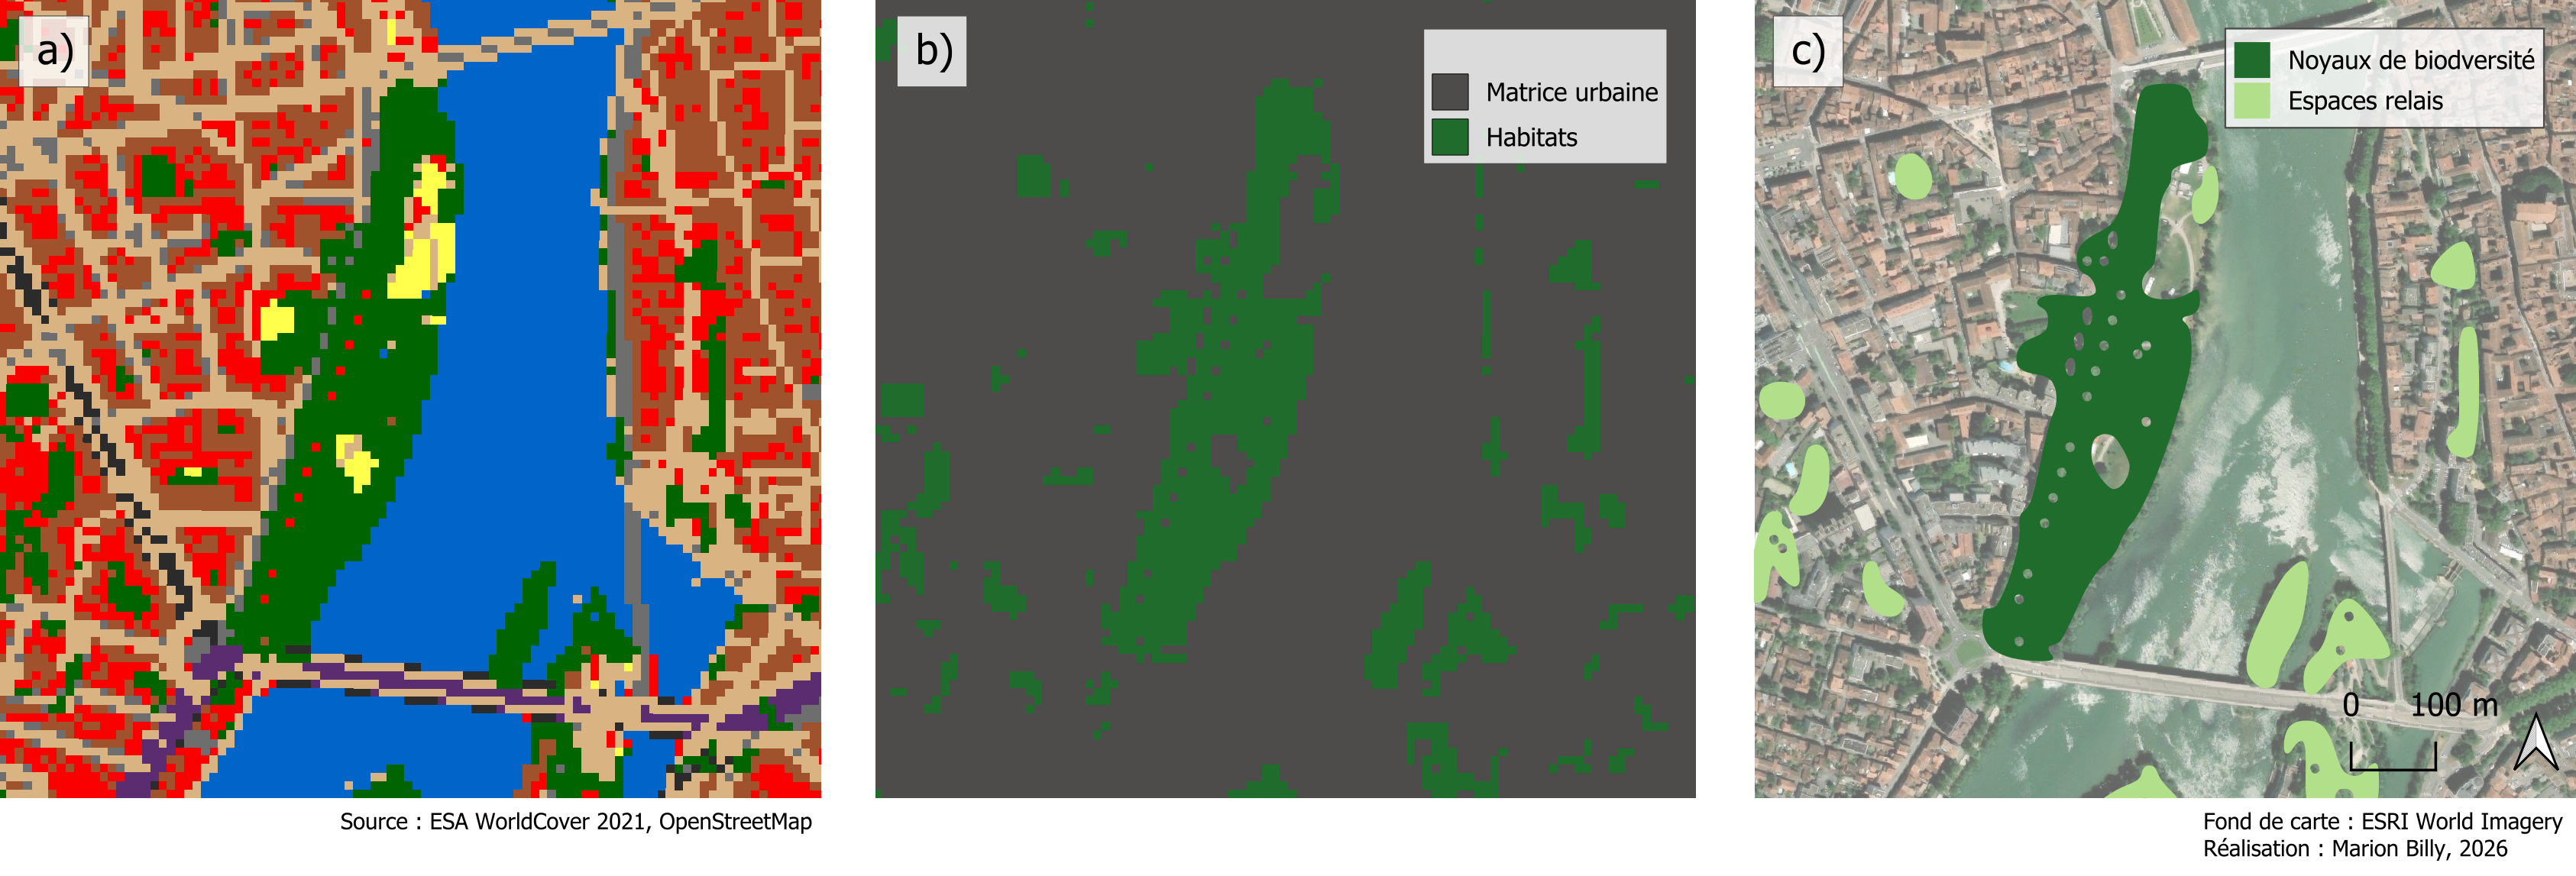
\includegraphics[width=\textwidth]{figures/steps_habitat_patches_fauvette.png}
\caption{Des taches d'habitat du profil fauvette sur le secteur des prairies des Filtres à Toulouse : (a) occupation du sol enrichie, (b) habitat binaire, (c) noyaux de biodiversité et espaces relais.}
\label{fig:mspa-perpignan}
\end{figure}

\subsection{Graphe de connectivité}
Ces taches deviennent alors les nœuds d'un graphe paysager, construit ici selon le critère de Gabriel. Deux taches sont reliées lorsque aucune autre ne s'intercale dans le cercle dont le segment les joignant constitue le diamètre (Gabriel \& Sokal, 1969), dans la limite d'une distance de recherche fixée à deux fois la distance caractéristique de dispersion du profil et mesurée de bord à bord.

À chaque lien est associée une probabilité de déplacement. Cette grandeur, qui revient dans tous les indicateurs de la chaîne, exprime la vraisemblance qu'un individu du profil écologique franchisse la distance séparant deux taches, proche de 1 pour des taches voisines et tendant vers 0 à mesure qu'elles s'éloignent. La forme retenue est un noyau négatif-exponentiel, standard des graphes paysagers depuis leurs premiers usages en écologie (Urban \& Keitt, 2001) et employé par les logiciels de référence du domaine (Saura \& Torné, 2009 ; Foltête et al., 2012). Il traduit par ailleurs une propriété observée de la dispersion, la décroissance rapide du nombre d'individus atteignant une distance donnée.

\begin{equation}\label{eq:pij}
p_{ij} = \exp\!\left(-\,d_{ij}/d_0\right)
\end{equation}

où $d_{ij}$ est la distance de bord à bord entre les taches $i$ et $j$, et $d_0$ la distance caractéristique de dispersion du profil, à laquelle la probabilité de déplacement retombe à environ 37 \% (soit $1/e$).

Le choix du graphe de Gabriel parmi les graphes de proximité conditionne les connexions retenues, et trois variantes ont été implémentées et comparées avant de trancher. L'arbre couvrant minimal relie toutes les taches avec la longueur totale de liens la plus faible, et le graphe de voisinage relatif (Toussaint, 1980) joint deux taches lorsque aucune autre n'est plus proche des deux à la fois : tous deux ne conservent qu'un unique chemin entre taches, sans redondance. Le graphe des $k$ plus proches voisins relie chaque tache à ses $k$ voisines, $k$ étant un paramètre arbitraire, au risque de sur- ou sous-connecter le réseau selon sa valeur. En écologie du paysage, l'arbre couvrant minimal sert de squelette, tandis qu'un graphe planaire plus dense représente le réseau tel qu'une espèce peut l'emprunter, avec ses chemins alternatifs (Fall et al., 2007). Le graphe de Gabriel conserve cette redondance sans relier deux taches qu'une troisième sépare.

Sur ce graphe est calculée la Probability of Connectivity (Saura \& Pascual-Hortal, 2007), qui mesure la connectivité potentielle à vol d'oiseau, indépendamment de la résistance du paysage.

\begin{equation}\label{eq:pc}
\mathrm{PC} = \frac{\displaystyle\sum_{i}\sum_{j} a_i\,a_j\,p_{ij}}{A^{2}}
\end{equation}

où $a_i$ et $a_j$ sont les surfaces des taches $i$ et $j$, $p_{ij}$ la probabilité de déplacement de l'équation~\eqref{eq:pij}, et $A$ la surface totale de la zone d'étude.

\subsection{Résistance du paysage et tracés de moindre coût}
La résistance du paysage est ensuite introduite, la surface de friction est dérivée de l'occupation du sol selon les coefficients du profil (Figure~\ref{fig:lcp-exemple}a et b ; annexe 3), puis chaque lien est tracé comme un chemin de moindre coût sur cette surface, au moyen de l'algorithme de coût cumulé géométrique de scikit-image (Figure~\ref{fig:lcp-exemple}c). Le coût de passage d'une cellule à sa voisine vaut la moyenne de leurs deux résistances, multipliée par la racine de deux lorsque le déplacement est diagonal, et le coût cumulé le long du trajet définit une distance effective, exprimée dans la même unité qu'une distance métrique. Calculer les tracés pour l'ensemble des couples retenus par le graphe, en bornant le calcul par un seuil propre à la capacité de dispersion du profil, correspond à l'application dite factorielle de l'analyse de moindre coût, développée pour lever la nécessité de désigner à l'avance les couples origine-destination (Diniz et al., 2020). Le chemin optimal en coût n'indique pas l'emprise d'un corridor à aménager mais l'endroit où un lien est le plus probable (Pinto \& Keitt, 2009 ; Shirabe, 2018), ce qui justifie de parler de lien ou de tracé de moindre coût plutôt que de corridor pour ces sorties.

Le coût cumulé de chaque lien est comparé à un budget de déplacement, fixé au triple de la distance caractéristique de dispersion du profil (Cerema Dter Sud-Ouest, 2025). Ce budget représente l'effort maximal qu'un individu peut consentir pour rejoindre une autre tache. Un déplacement de trois kilomètres en milieu parfaitement perméable mobilise ainsi le même budget qu'un déplacement d'un kilomètre à travers des milieux trois fois plus résistants. Ce facteur fixe le seuil de fonctionnalité. En deçà, le lien est jugé fonctionnel. Au-delà, ou s'il rencontre un obstacle infranchissable, il est marqué en échec. Une carte de dispersion complète ce dispositif (Figure~\ref{fig:lcp-exemple}d) : surface de coût cumulé propagé depuis l'ensemble des taches sources et bornée au budget de déplacement, qui représente l'étendue qu'un profil peut atteindre depuis son habitat.

\begin{figure}[H]
\centering
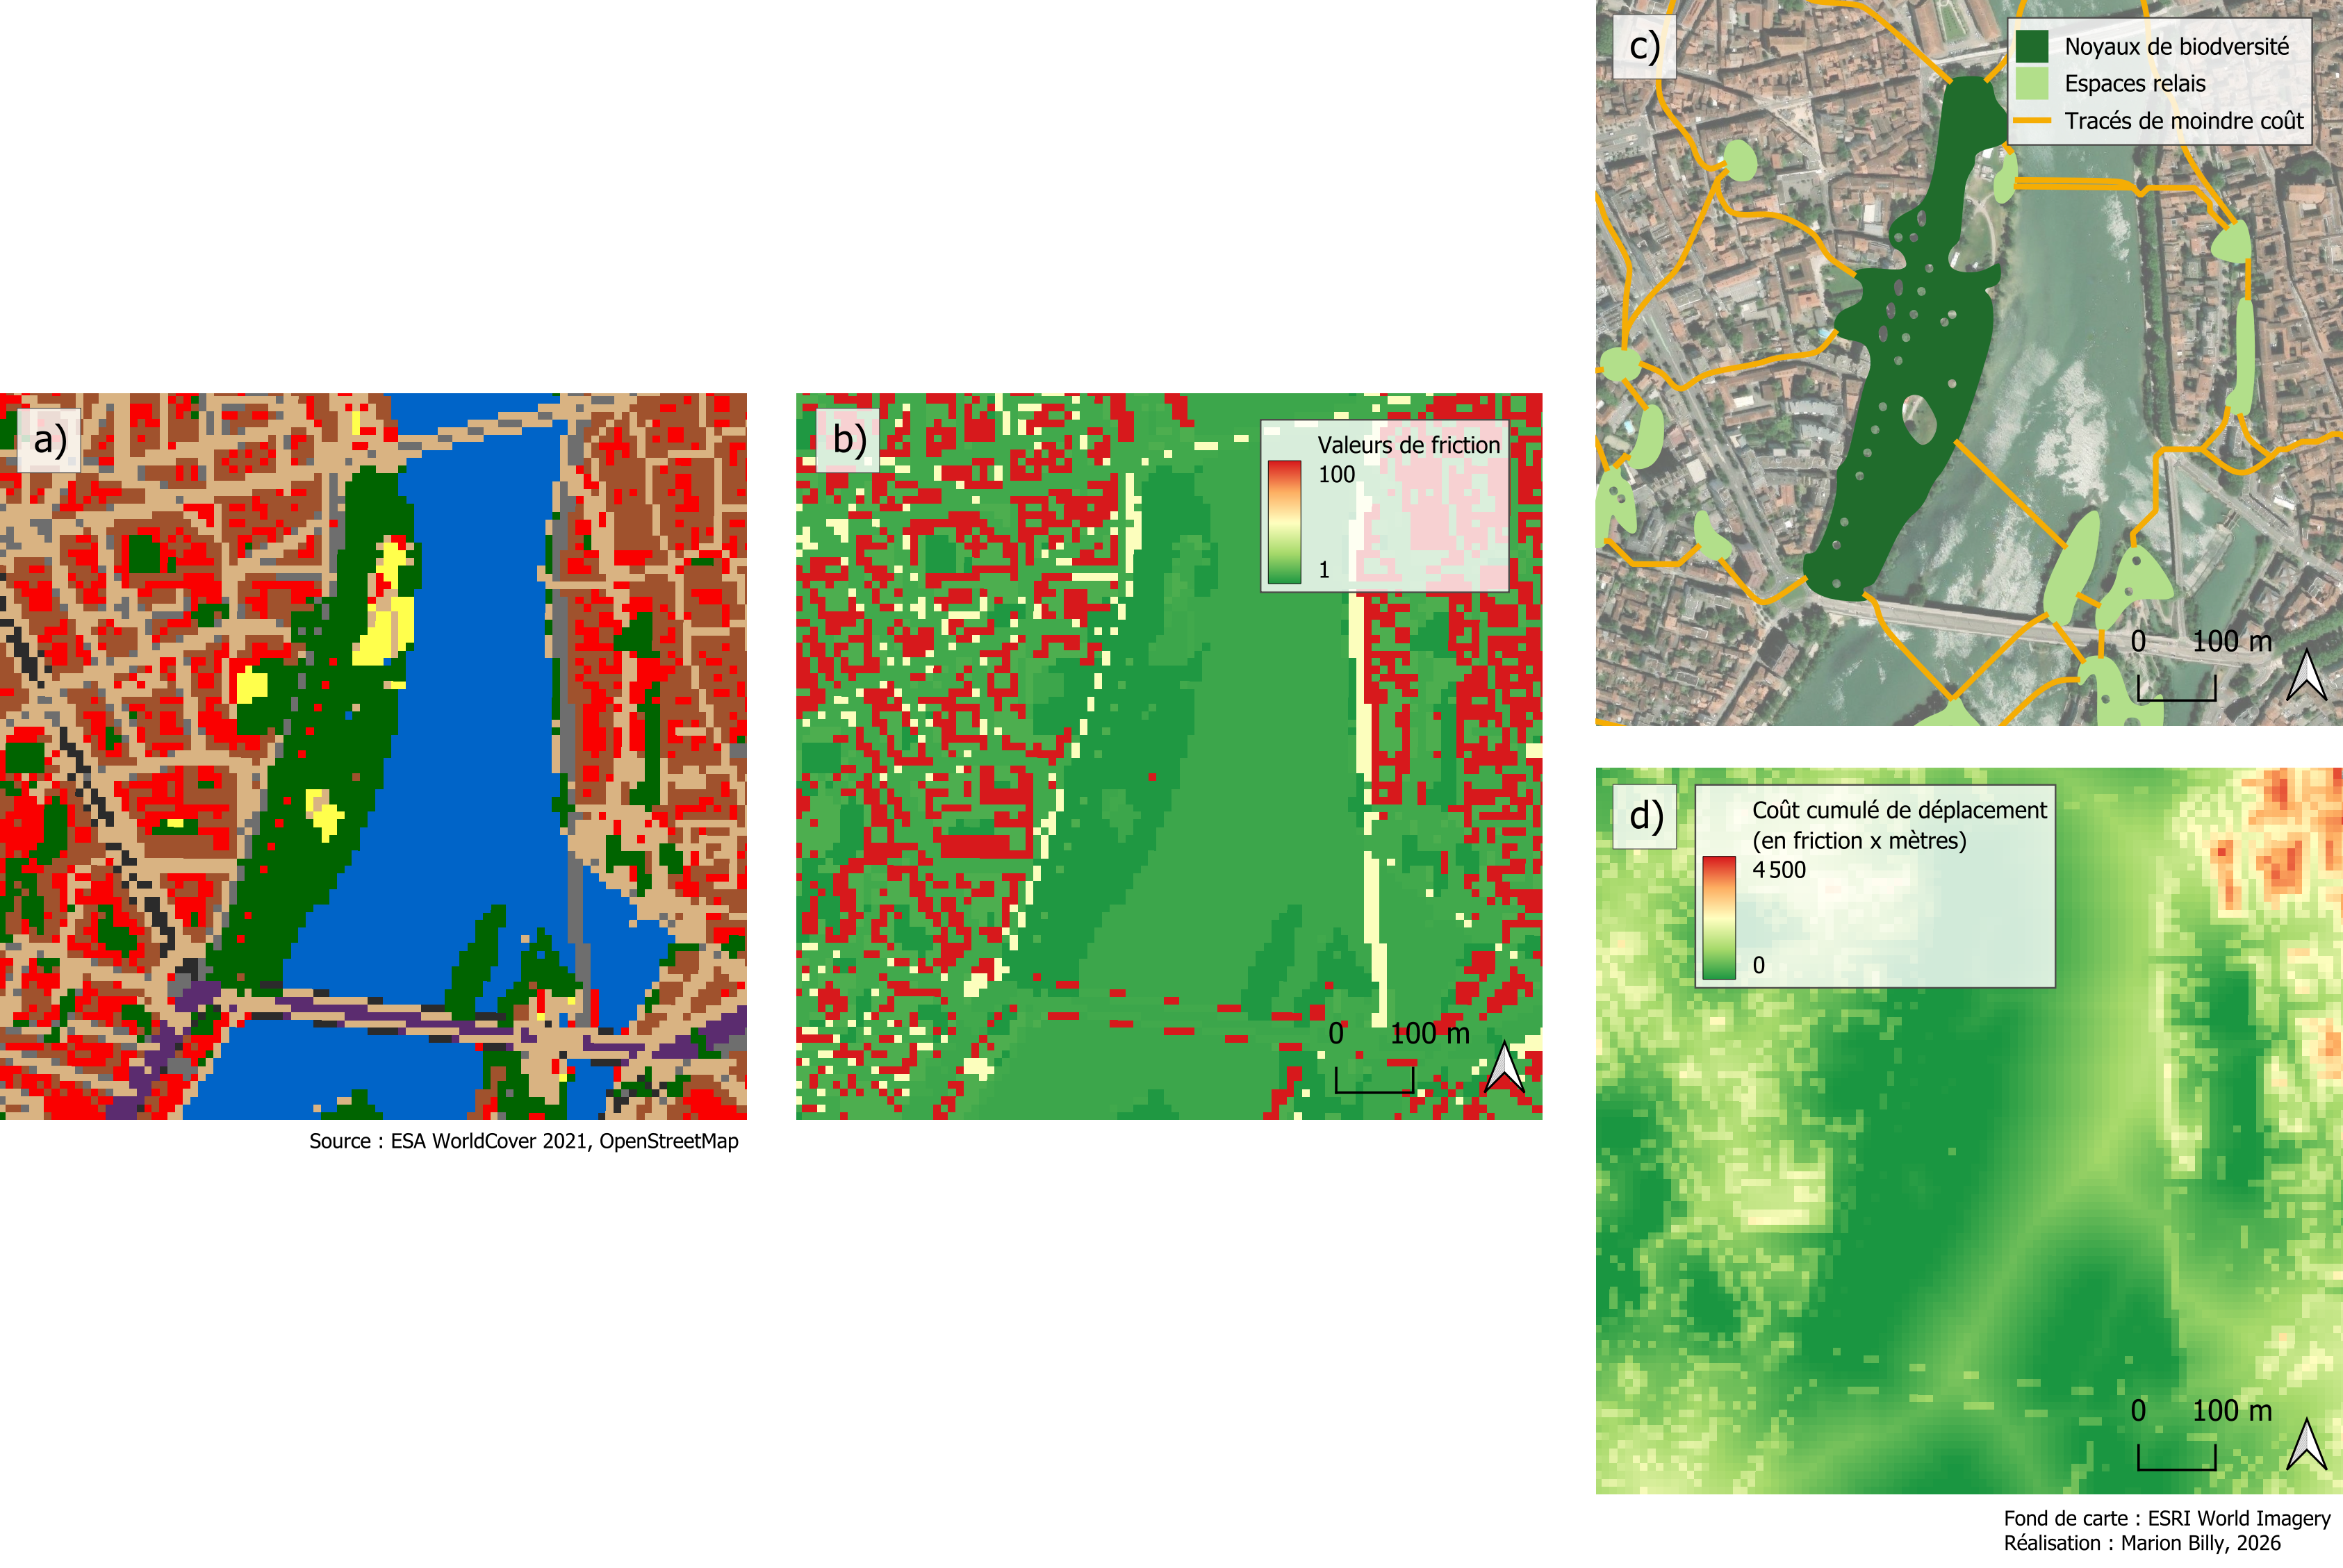
\includegraphics[width=\textwidth]{figures/steps4_lcp_fauvette.png}
\caption{Du sol au tracé de moindre coût, profil fauvette sur le secteur des prairies des Filtres à Toulouse : (a) occupation du sol, (b) friction, (c) noyaux de biodiversité, espaces relais et tracés de moindre coût, (d) coût cumulé de déplacement en partant des taches sources.}
\label{fig:lcp-exemple}
\end{figure}

Deux filtres se combinent donc pour décider qu'un lien existe, le plafond géométrique du graphe, qui borne les paires de taches examinées (§2.4.2), et le budget de coût, qui valide ou écarte chaque lien examiné. Le second est le critère déterminant, puisqu'il tient compte de la nature des milieux traversés, alors que le premier ne considère que la distance.

\subsection{Indicateurs}
Plusieurs indicateurs caractérisent l'état du réseau. La Probability of Connectivity est recalculée sur le réseau tracé, en remplaçant la distance en ligne droite l'équation~\eqref{eq:pij} par le coût cumulé du tracé. Un lien bloqué par un obstacle infranchissable reçoit une probabilité nulle, et un lien dont le coût excède le budget de déplacement conserve une probabilité résiduelle très faible (inférieure à $e^{-3}$, soit environ 0,05). Cette nouvelle valeur mesure ainsi la connectivité réelle du réseau, tenant compte des obstacles du paysage, là où la version initiale ne mesurait qu'une connectivité géométrique à vol d'oiseau. La surface équivalente connectée (Equivalent Connected Area ; Saura et al., 2011) la traduit en unité de surface :

\begin{equation}\label{eq:ec}
\mathrm{EC} = \sqrt{\mathrm{PC}} \times A
\end{equation}

L'EC s'interprète comme la taille d'un unique bloc d'habitat parfaitement connecté qui aurait la même PC que le réseau réel. Exprimée en hectares, elle est plus parlante pour un aménageur que la probabilité dont elle dérive. La part d'habitat connecté en découle : c'est le rapport de cette surface équivalente à la surface totale d'habitat du territoire, exprimé en pourcentage. Deux indicateurs complètent la lecture. Le nombre de sous-réseaux correspond au nombre de composantes connexes du réseau des liens fonctionnels, comptées sur les seules taches de la zone d'étude stricte ; un groupe de moins de trois taches n'est pas compté comme sous-réseau. Un réseau connexe forme un seul ensemble relié, tandis que plusieurs sous-réseaux traduisent un réseau fragmenté en parties non reliées entre elles. La tortuosité des tracés rapporte leur longueur réelle à la distance en ligne droite : proche de 1, le tracé est quasi rectiligne et peu contraint. Élevée, elle indique un contournement par de longs détours, signe d'une matrice résistante.

\subsection{Sorties}
La chaîne produit pour chaque couple quatre couches cartographiques et un tableau d'indicateurs. Les noyaux de biodiversité et les espaces relais localisent l'habitat (§2.4.1). Les liens fonctionnels, tracés de moindre coût dont le coût cumulé reste dans le budget du profil, désignent les passages probables entre taches (§2.4.3). Les surfaces de dispersion délimitent l'étendue atteignable depuis l'habitat. Une couche intermédiaire recense les connexions recherchées mais non réalisables, non destinée à l'affichage puisque la représenter reviendrait à tracer des liens que le modèle a écartés.

\begin{figure}[H]
\centering
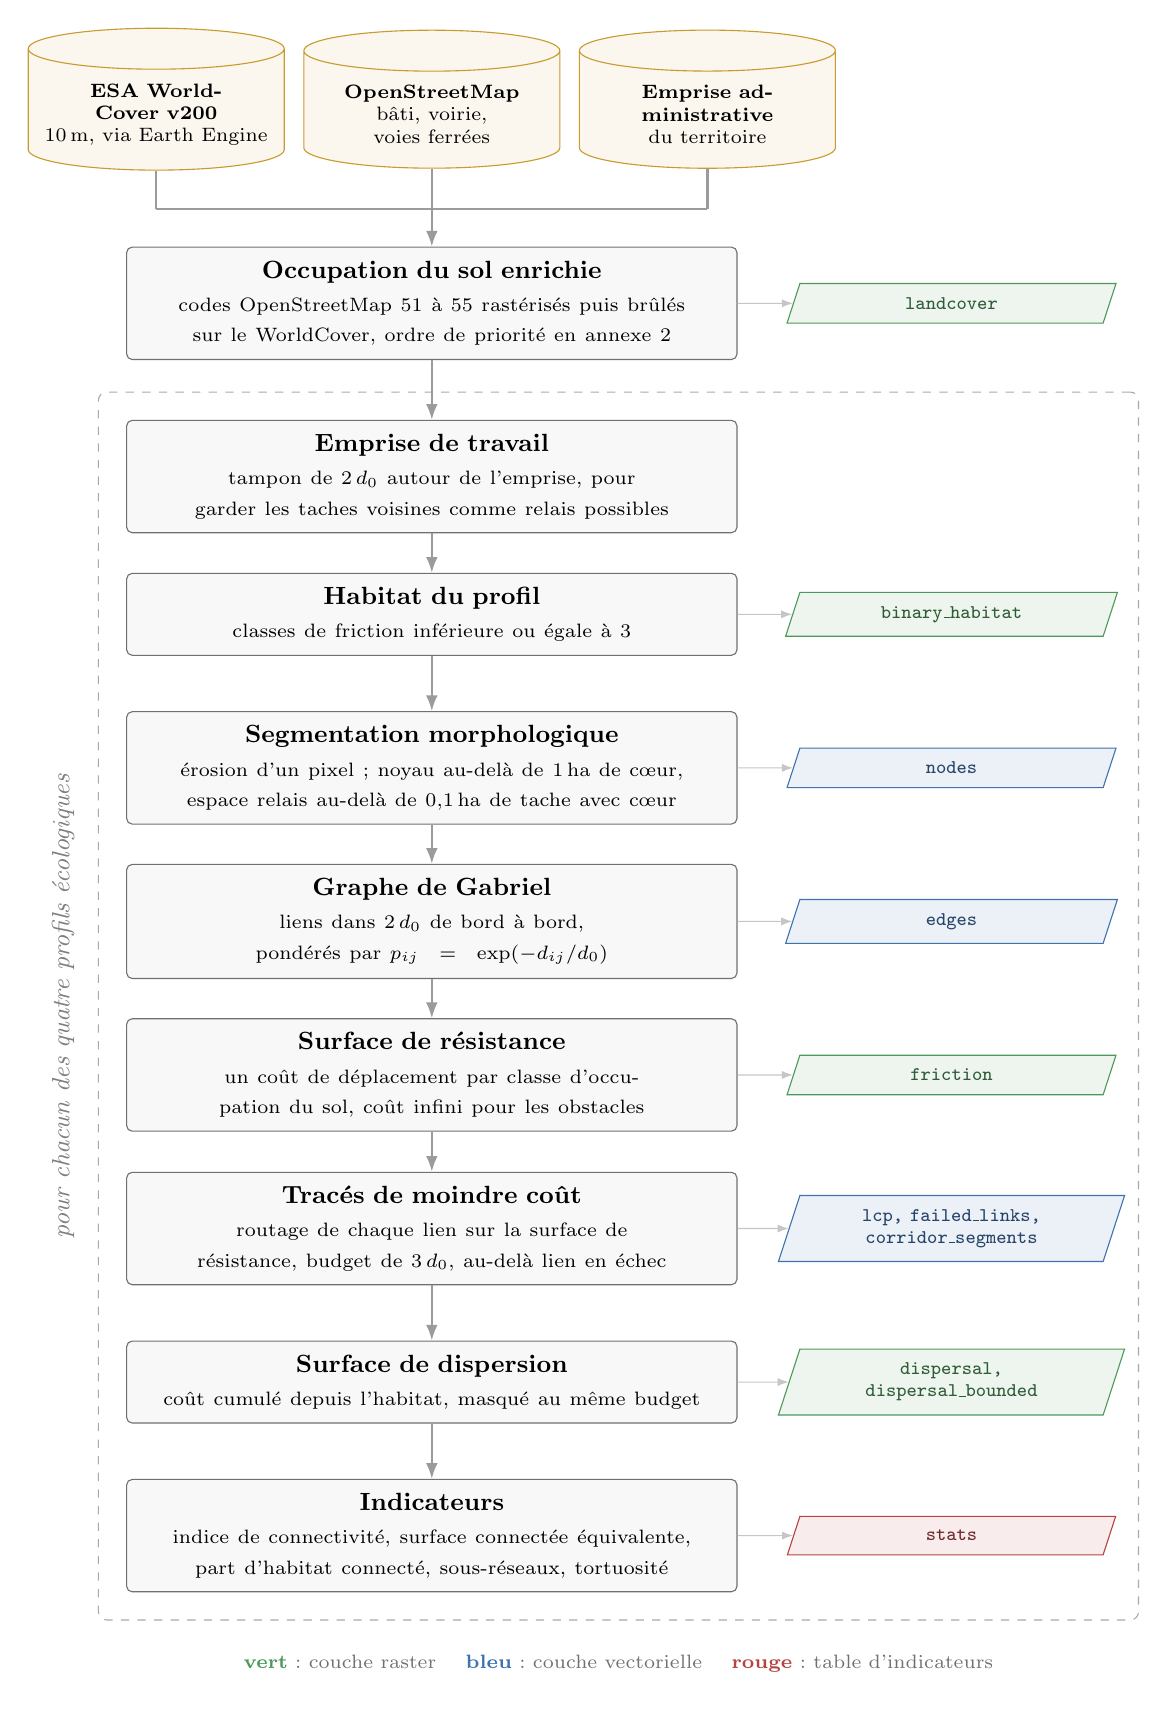
\begin{tikzpicture}[
  font=\small,
  cadre/.style={rounded corners=2pt, align=center, inner sep=5pt},
  % formes conventionnelles du logigramme : le cylindre désigne un jeu de
  % données, le rectangle un traitement, le parallélogramme une donnée produite
  entreeb/.style={cylinder, shape border rotate=90, aspect=0.16, draw=entree,
                  fill=entree!8, align=center, inner sep=5pt, text width=2.9cm,
                  font=\scriptsize},
  etape/.style={cadre, draw=etapec, fill=etapec!5, text width=7.4cm},
  rast/.style={trapezium, trapezium left angle=72, trapezium right angle=108,
               trapezium stretches body, draw=raster, fill=raster!10,
               align=center, inner sep=5pt, text width=3.5cm,
               font=\scriptsize\ttfamily, text=raster!60!black},
  vect/.style={trapezium, trapezium left angle=72, trapezium right angle=108,
               trapezium stretches body, draw=vecteur, fill=vecteur!10,
               align=center, inner sep=5pt, text width=3.5cm,
               font=\scriptsize\ttfamily, text=vecteur!60!black},
  tabl/.style={trapezium, trapezium left angle=72, trapezium right angle=108,
               trapezium stretches body, draw=tablec, fill=tablec!10,
               align=center, inner sep=5pt, text width=3.5cm,
               font=\scriptsize\ttfamily, text=tablec!60!black},
  fl/.style={-{Latex[length=2mm]}, etapec!70, thick},
  fll/.style={-{Latex[length=1.4mm]}, etapec!40},
]
% ---- entrées, une fois par territoire
\node[entreeb] (e1) at (-3.5,0.4) {\textbf{ESA WorldCover v200}\\10\,m, via Earth Engine};
\node[entreeb] (e2) at (0,0.4) {\textbf{OpenStreetMap}\\bâti, voirie, voies ferrées};
\node[entreeb] (e3) at (3.5,0.4) {\textbf{Emprise administrative}\\du territoire};
\node[etape] (s0) at (0,-2.0)
  {\textbf{Occupation du sol enrichie}\\[1pt]\scriptsize codes OpenStreetMap 51 à 55 rastérisés puis brûlés sur le WorldCover, ordre de priorité en annexe 2};
\draw[etapec!70, thick] (e1.south) -- (-3.5,-0.8);
\draw[etapec!70, thick] (e2.south) -- (0,-0.8);
\draw[etapec!70, thick] (e3.south) -- (3.5,-0.8);
\draw[etapec!70, thick] (-3.5,-0.8) -- (3.5,-0.8);
\draw[fl] (0,-0.8) -- (s0);
\node[rast] (o0) at (6.6,-2.0) {landcover};
% ---- boucle sur les quatre profils écologiques
\node[etape] (s1) at (0,-4.2)
  {\textbf{Emprise de travail}\\[1pt]\scriptsize tampon de $2 \, d_0$ autour de l'emprise, pour garder les taches voisines comme relais possibles};
\node[etape] (s2) at (0,-5.95)
  {\textbf{Habitat du profil}\\[1pt]\scriptsize classes de friction inférieure ou égale à 3};
\node[rast] (o2) at (6.6,-5.95) {binary\_habitat};
\node[etape] (s3) at (0,-7.9)
  {\textbf{Segmentation morphologique}\\[1pt]\scriptsize érosion d'un pixel ; noyau au-delà de 1\,ha de cœur, espace relais au-delà de 0,1\,ha de tache avec cœur};
\node[vect] (o3) at (6.6,-7.9) {nodes};
\node[etape] (s4) at (0,-9.85)
  {\textbf{Graphe de Gabriel}\\[1pt]\scriptsize liens dans $2 \, d_0$ de bord à bord, pondérés par $p_{ij} = \exp(-d_{ij}/d_0)$};
\node[vect] (o4) at (6.6,-9.85) {edges};
\node[etape] (s5) at (0,-11.8)
  {\textbf{Surface de résistance}\\[1pt]\scriptsize un coût de déplacement par classe d'occupation du sol, coût infini pour les obstacles};
\node[rast] (o5) at (6.6,-11.8) {friction};
\node[etape] (s6) at (0,-13.75)
  {\textbf{Tracés de moindre coût}\\[1pt]\scriptsize routage de chaque lien sur la surface de résistance, budget de $3 \, d_0$, au-delà lien en échec};
\node[vect] (o6) at (6.6,-13.75) {lcp, failed\_links,\\corridor\_segments};
\node[etape] (s7) at (0,-15.7)
  {\textbf{Surface de dispersion}\\[1pt]\scriptsize coût cumulé depuis l'habitat, masqué au même budget};
\node[rast] (o7) at (6.6,-15.7) {dispersal,\\dispersal\_bounded};
\node[etape] (s8) at (0,-17.65)
  {\textbf{Indicateurs}\\[1pt]\scriptsize indice de connectivité, surface connectée équivalente, part d'habitat connecté, sous-réseaux, tortuosité};
\node[tabl] (o8) at (6.6,-17.65) {stats};
\draw[fl] (s0) -- (s1);
\draw[fl] (s1) -- (s2);
\draw[fl] (s2) -- (s3);
\draw[fl] (s3) -- (s4);
\draw[fl] (s4) -- (s5);
\draw[fl] (s5) -- (s6);
\draw[fl] (s6) -- (s7);
\draw[fl] (s7) -- (s8);
\draw[fll] (s0.east) -- (o0.west);
\draw[fll] (s2.east) -- (o2.west);
\draw[fll] (s3.east) -- (o3.west);
\draw[fll] (s4.east) -- (o4.west);
\draw[fll] (s5.east) -- (o5.west);
\draw[fll] (s6.east) -- (o6.west);
\draw[fll] (s7.east) -- (o7.west);
\draw[fll] (s8.east) -- (o8.west);
% ---- le cadre de la boucle
\begin{scope}[on background layer]
\node[draw=etapec!60, dashed, rounded corners=3pt, inner sep=10pt,
      fit=(s1)(s8)(o2)(o8)] (boucle) {};
\end{scope}
% le libellé de la boucle se lit à la verticale, à gauche du cadre : au-dessus, il
% passait sous la boîte de l'occupation du sol
\node[rotate=90, anchor=south, font=\small\itshape, text=etapec!90]
  at ([xshift=-5pt]boucle.west)
  {pour chacun des quatre profils écologiques};
% ---- légende des couleurs
\node[anchor=north, font=\scriptsize, text width=11cm, align=center,
      text=etapec] at ([yshift=-9pt]boucle.south)
  {\textcolor{raster}{\textbf{vert}} : couche raster \quad \textcolor{vecteur}{\textbf{bleu}} : couche vectorielle \quad \textcolor{tablec}{\textbf{rouge}} : table d'indicateurs};
\end{tikzpicture}
\caption{Vue d'ensemble de la chaîne de traitement, des entrées aux couches produites.}
\label{fig:pipeline}
\end{figure}

\section{Implémentation, contrôle des sorties et reproductibilité}
La chaîne est implémentée intégralement en Python, sans recours à un logiciel de SIG externe ni à un outil de connectivité existant. Les outils existants de connectivité, Graphab, Conefor ou Circuitscape, prennent en entrée un graphe de taches d'habitat et en calculent les métriques. Le service visé demande un périmètre plus large : en amont, l'acquisition des images et la dérivation de l'occupation du sol propre à chaque profil ; en aval, les indicateurs, les couches prêtes pour le tableau de bord et la comparaison de scénarios. Les intégrer à cet ensemble demanderait une préparation manuelle des couches, territoire par territoire, quand l'objectif est un enchaînement complet en une commande unique. Un développement dédié en Python assure cette continuité et le contrôle sur chaque étape.

Les traitements raster reposent sur xarray et rioxarray, les traitements vectoriels sur geopandas et shapely, la rastérisation sur rasterio, le graphe sur networkx et scipy, et les calculs de moindre coût et de morphologie sur scikit-image (versions en annexe 4). La pile géospatiale, geopandas, shapely, rasterio et xarray, correspond aux bibliothèques déjà utilisées en interne par l'équipe, ce qui a guidé leur choix pour cette chaîne. Le recours à scikit-image pour le moindre coût tient à l'adéquation fonctionnelle : la fonction employée pondère les déplacements diagonaux selon leur longueur réelle, propage le coût depuis un ensemble de pixels sources, ce qu'exigent les surfaces de dispersion, et reconstruit le trajet emprunté. La répartition entre networkx et scipy résulte d'une mesure, networkx assurant la construction et la topologie du graphe et scipy le calcul des plus courts chemins.

Un script unique pilote l'exécution et écrit pour chaque couple territoire-profil une arborescence de sorties identiques d'un territoire à l'autre : rasters d'occupation du sol, d'habitat, de friction et de dispersion, couches vectorielles des nœuds, tracés de moindre coût, enfin tableau d'indicateurs. Le code est versionné dans un \href{https://github.com/marion-billy/urbiverde_ivb}{dépôt GitHub}, qui rassemble les modules de traitement, le fichier de configuration des profils écologiques, les tests et la documentation de suivi ; les sorties, volumineuses, en sont exclues. Les versions des bibliothèques employées sont relevées dans l'environnement d'exécution et figées dans le dépôt (annexe 4).

La chaîne ne comporte aucun tirage aléatoire : relancée sur le même territoire à partir du même instantané d'occupation du sol, une même commande produit des sorties identiques. Cela a été vérifié, deux exécutions successives livrent des fichiers rigoureusement identiques sur l'ensemble des couches et sur des indicateurs. OpenStreetMap est une base modifiée quotidiennement, et n'offre pas de version citable. Reproduire des résultats suppose donc de rejouer la chaîne sur le même instantané d'entrée, elle archive donc les données pour les six territoires plutôt que de réinterroger le réseau à chaque exécution.

Un contrôle automatisé s'exécute à la fin de chaque traitement et vérifie que toutes les couches attendues ont été écrites et comportent les champs prévus, qu'aucune n'est vide, que la projection est bien celle du territoire, et que les valeurs restent dans leurs bornes admissibles. Toute anomalie est signalée avant que les sorties ne soient exploitées. 

Ce contrôle porte sur les sorties produites. Il est complété par une suite de tests de non-régression portant sur les fonctions de calcul : chacune reçoit une entrée réduite dont la réponse se calcule à la main, et le test vérifie qu'elle la produit. Par exemple, sur un graphe de deux taches reliées par un lien de probabilité 0,5, le test vérifie que l'équation~\eqref{eq:pc} donne 0,75, contre 0,50 en l'absence de lien. Ce test garantit que des modifications ultérieures du code ne déplacent pas le résultat. Les autres tests agissent de façon similaire et portent sur la binarisation de l'habitat, la tortuosité, la conversion des obstacles en coût infini et les seuils de la segmentation morphologique. Trois tests enfin ne portent pas sur le code mais sur la configuration, vérifiant que les règles de calibration énoncées en annexe 3 sont bien celles qu'applique le fichier de paramètres : friction d'un code d'habitat inférieure ou égale à trois, obstacles infranchissables pour les profils annoncés, budget de déplacement égal à trois fois la distance de dispersion. Une modification des paramètres qui contredirait les règles fixées est ainsi détectée. 

Le code suit les conventions de l'équipe, formalisées dans un document interne : chaque fonction est documentée et ses types annotées, et le nommage et l'organisation des fichiers vérifiés par un script d'audit de conformité. Le style respecte la norme PEP-8, contrôlée ponctuellement par un analyseur statique et non à chaque modification : l'automatisation de ces vérifications fait partie des travaux d'industrialisation restant à conduire.

\section{Restitution : le tableau de bord}
La restitution de ces sorties prend la forme d'un tableau de bord interactif, qui présente pour chaque territoire et chaque profil les couches produites, que l'utilisateur peut afficher et superposer, ainsi que les indicateurs associés. Il donne accès à une exploration visuelle du réseau écologique d'un territoire et à la simulation de scénarios d'aménagement (Figure~\ref{fig:dashboard}). C'est une application web développée en Python avec Plotly Dash, l'affichage des cartes reposant sur Leaflet, bâtie sur les gabarits de Murmuration et versionnée dans le dépôt GitLab interne. Les géométries et les indicateurs sont repris tels quels aux formats GeoJSON et CSV, après simplification des tracés. Le raster de dispersion, trop lourd pour un navigateur, est précalculé en une image colorisée légère embarquée avec l'application. À la fin du stage, la version en état de marche s'exécute en local : le déploiement dans l'environnement de l'entreprise suppose une industrialisation du code qui n'a pas été menée dans le temps imparti, et l'intégration à la plateforme UrbiVerde reste à réaliser. Le tableau de bord constitue donc un prototype. 

La répartition du travail sur le dashboard mérite d'être précisée. J'ai produit les sorties, défini le contenu à présenter et réalisé une maquette ; l'application elle-même a été développée par des collègues, l'entreprise disposant d'une équipe spécialisée dans les interfaces et les tableaux de bord. Je n'y ai ensuite apporté que quelques modifications ponctuelles, avec l'assistance de l'agent de programmation mentionné au §5.3.

\begin{figure}[H]
\centering
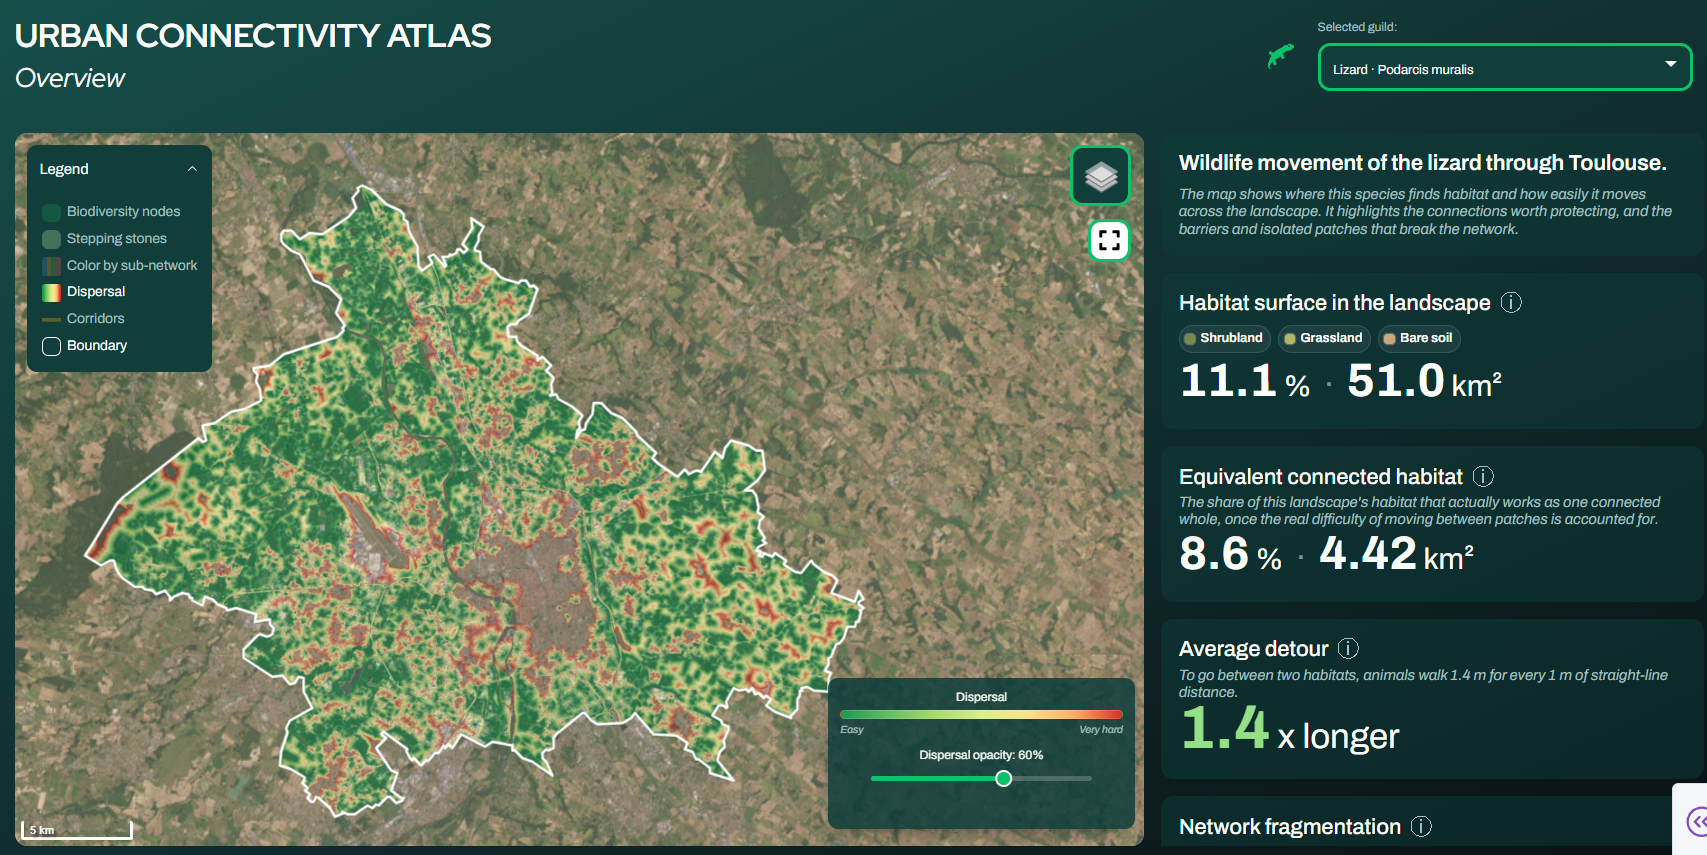
\includegraphics[width=\textwidth]{figures/dashboard1.png}\\[0.35cm]
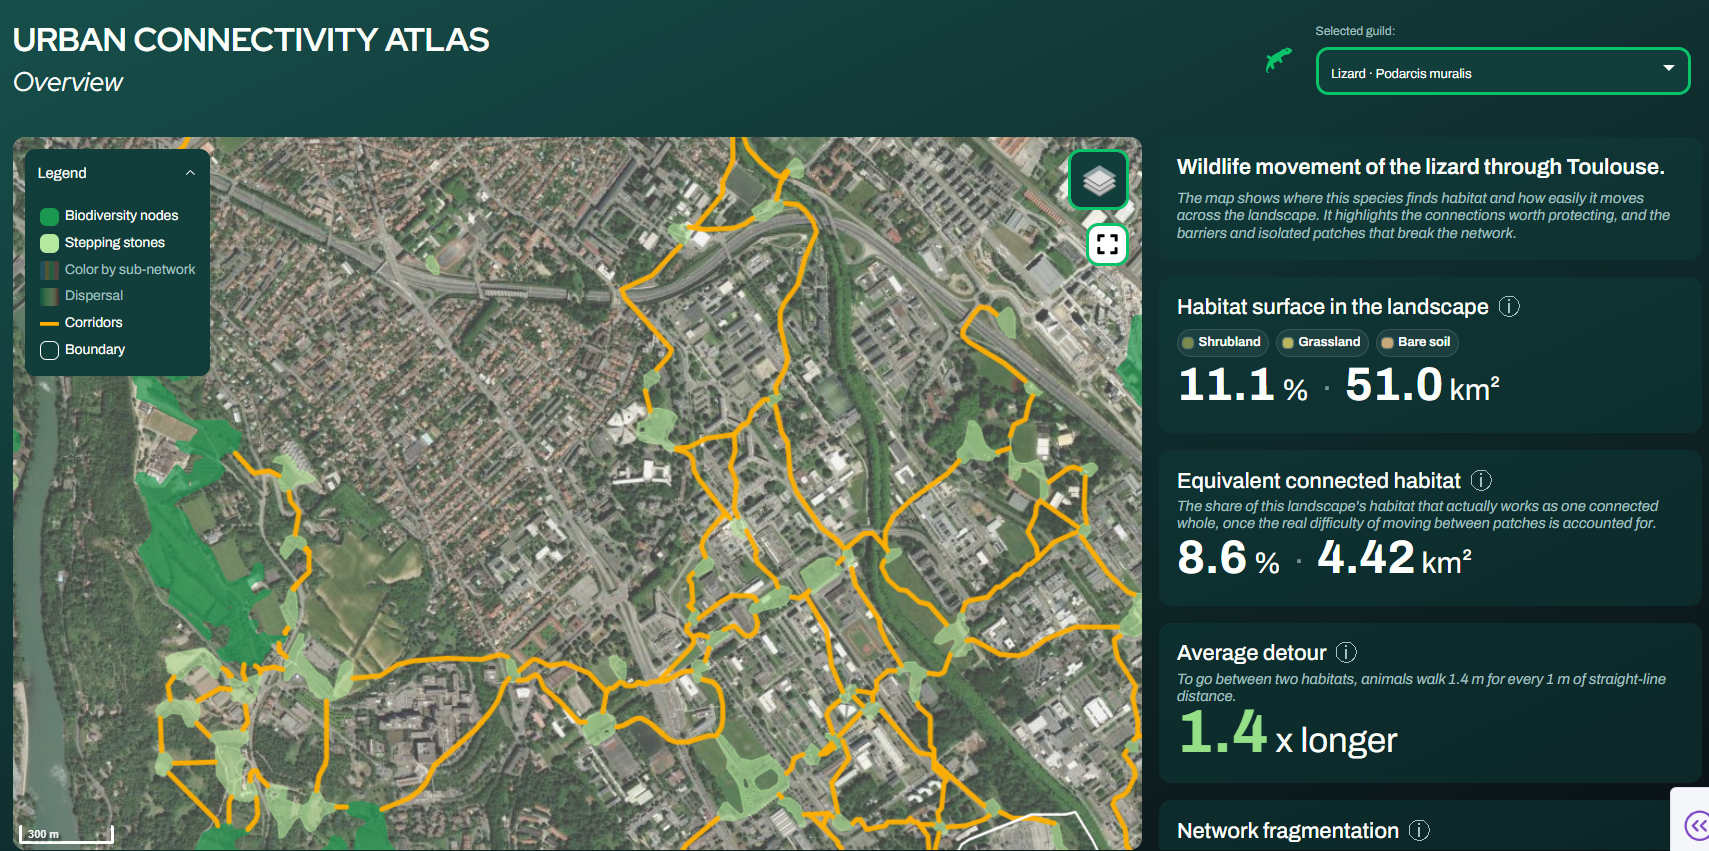
\includegraphics[width=\textwidth]{figures/dashboard2.png}
\caption{Tableau de bord interactif, profil lézard sur Toulouse : surface de dispersion à l'échelle du territoire (haut), noyaux de biodiversité, espaces relais et tracés de moindre coût à l'échelle du quartier (bas). Sélecteur de profil en haut à droite, indicateurs de connectivité associés en colonne de droite.}
\label{fig:dashboard}
\end{figure}

\section{Protocoles d'évaluation}
La chaîne de traitement est évaluée sous deux angles complémentaires : la stabilité de ses conclusions face aux paramètres les moins établis (analyse de sensibilité, §2.7.1) et la cohérence de ses couches avec des observations d'espèces indépendantes (§2.7.2).

\subsection{Analyse de sensibilité}
L'analyse de sensibilité étudie comment les sorties d'un modèle se modifient lorsque ses paramètres varient. Elle permet de séparer ce qui résulte du paysage analysé et ce qui résulte des valeurs choisies pour paramétrer le modèle. Elle porte ici sur les coefficients de friction et les distances de dispersion, car ce sont celles qui reposent sur des valeurs de référence issues de la littérature transposées à des territoires pour lesquels elles n'ont pas été établies.

Deux dispositifs complémentaires ont été mis en œuvre (Figure~\ref{fig:schema-sensibilite}). Un balayage sur plage large, portant sur la distance de dispersion et sur le contraste de friction, c'est-à-dire l'écart de coût entre habitat et matrice, indique à partir de quelle valeur le diagnostic change de nature. Les balayages parcourent \{50, 60, 70, 75, 80, 90, 110, 120\} \% de la distance de dispersion de référence et \{0, 25, 50, 75, 125, 150, 200\} \% du contraste de friction. Une perturbation locale, un facteur à la fois, hiérarchise ensuite les paramètres au voisinage des valeurs retenues. Ses amplitudes, 20 \% sur les coefficients de friction et 25 \% sur la distance de dispersion, ont été fixées au vu des balayages : elles restent à l'intérieur du domaine où le diagnostic est stable, tout en représentant l'ordre de grandeur d'une erreur de calibration plausible. 

\begin{figure}[H]
\centering
\resizebox{\textwidth}{!}{%
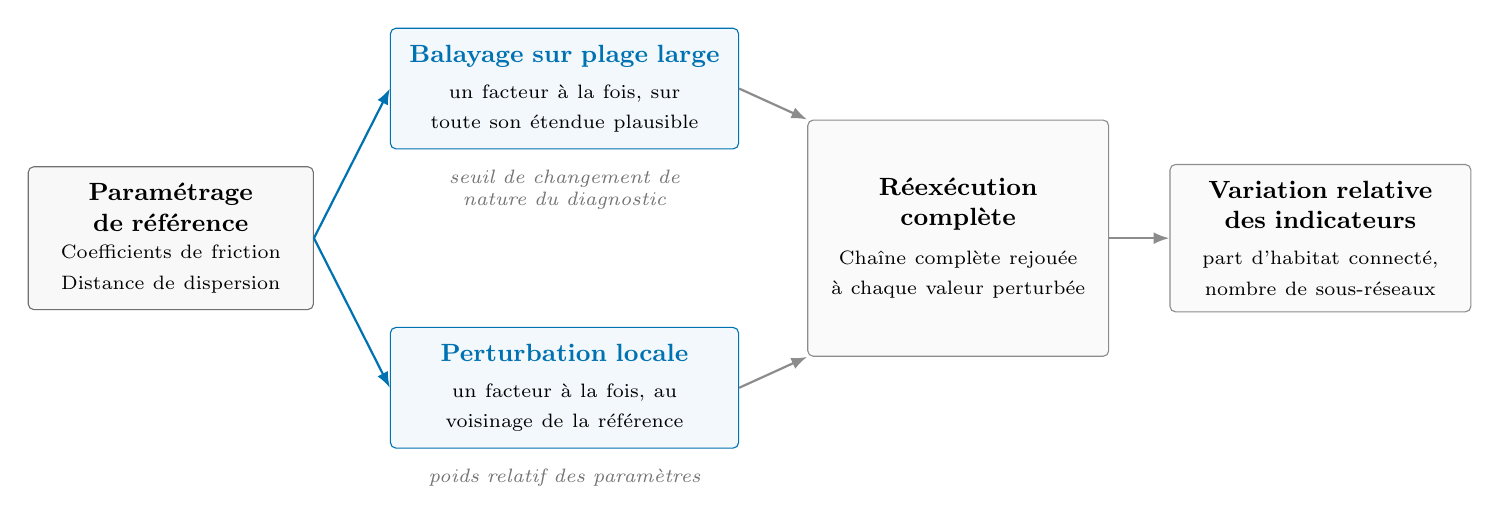
\begin{tikzpicture}[
  font=\small,
  cadre/.style={rounded corners=2pt, align=center, inner sep=6pt},
  ref/.style={cadre, draw=etapec, fill=etapec!5, text width=3.2cm},
  disp/.style={cadre, draw=cible, fill=cible!5, text width=4.0cm},
  etape/.style={cadre, draw=black!45, fill=black!2, text width=3.4cm},
  mesure/.style={rounded corners=2pt, align=center, inner sep=4pt, text width=3.0cm,
                 font=\scriptsize, draw=etapec!60, fill=etapec!8},
  fl/.style={-{Latex[length=2mm]}, black!45, thick},
]
% le point de départ commun
\node[ref] (ref) at (0,0)
  {\textbf{Paramétrage de référence}\\[2pt]\scriptsize Coefficients de friction\\Distance de dispersion};
% les deux dispositifs
\node[disp] (loc) at (5.0,-1.9)
  {\textbf{\textcolor{cible}{Perturbation locale}}\\[2pt]\scriptsize un facteur à la fois, au voisinage de la référence};
\node[disp] (bal) at (5.0,1.9)
  {\textbf{\textcolor{cible}{Balayage sur plage large}}\\[2pt]\scriptsize un facteur à la fois, sur toute son étendue plausible};
\node[anchor=north, font=\scriptsize\itshape, text=black!55,
       text width=4.2cm, align=center] at ([yshift=-4pt]loc.south)
  {poids relatif des paramètres};
\node[anchor=north, font=\scriptsize\itshape, text=black!55,
       text width=4.2cm, align=center] at ([yshift=-4pt]bal.south)
  {seuil de changement de nature du diagnostic};
% l'étape commune
\node[etape, minimum height=3.0cm] (rerun) at (10.0,0)
  {\textbf{Réexécution complète}\\[3pt]\scriptsize Chaîne complète rejouée à chaque valeur perturbée};
% la grandeur de stabilité
\node[etape] (mes) at (14.6,0)
  {\textbf{Variation relative des indicateurs}\\[2pt]\scriptsize part d'habitat connecté, nombre de sous-réseaux};
% flux
\draw[fl, cible] (ref.east) -- (loc.west);
\draw[fl, cible] (ref.east) -- (bal.west);
\draw[fl] (loc.east) -- (rerun.south west);
\draw[fl] (bal.east) -- (rerun.north west);
\draw[fl] (rerun) -- (mes);
\end{tikzpicture}}
\caption{Les deux dispositifs de l'analyse de sensibilité, du paramétrage de référence à la mesure de stabilité. Réalisation personnelle.}
\label{fig:schema-sensibilite}
\end{figure}

La stabilité des sorties est mesurée par la variation relative des indicateurs, de combien se déplacent la part d'habitat connecté et le nombre de sous-réseaux. Les plages parcourues couple par couple figurent en annexe 7.

Deux limites l'encadrent. Chaque exécution perturbée demandant un traitement complet du territoire, les balayages couvrent les vingt-quatre couples territoire-profil quand la perturbation locale se limite à quatre d'entre eux, un profil très mobile et un profil contraint sur deux tissus contrastés. Et la stabilité au paramétrage ne renseigne pas sur l'accord des sorties avec les déplacements réels (§4.2).

\subsection{Confrontation aux occurrences d'espèces}
La confrontation aux occurrences d'espèces GBIF porte sur un aspect précis du modèle : elle examine si les espèces que représente un profil écologique sont effectivement observées là où le modèle place son habitat. Elle ne teste pas les déplacements, des occurrences ne renseignant pas le mouvement d'un individu d'une tache à l'autre, si bien que ni le tracé des liens, ni leur coût ne peuvent être vérifiés par cette voie. Les couches produites sont confrontées aux occurrences de quatre espèces par profil écologique, sur les cinq territoires métropolitains. Ces espèces partagent avec l'espèce repère du profil ses exigences d'habitat et son ordre de grandeur de capacité de déplacement, et sont assez communes pour que les bases en contiennent un effectif exploitable (liste en annexe 8). Les relevés sont filtrés aux seules observations humaines postérieures à 2016 dont l'incertitude de localisation ne dépasse pas 100 mètres, seuil courant de nettoyage des occurrences (Zizka et al., 2019), puis amincis à une occurrence par cellule de dix mètres et par taxon. Chaque occurrence est ensuite affectée à l'une des quatre couches selon une règle de priorité, noyau, espace relais, tracé de moindre coût, matrice. Les tracés étant des lignes sans largeur, leur emprise est matérialisée par un tampon de vingt-cinq mètres. Pour distinguer ce qui relève d'une préférence de l'espèce et ce qui relève de la répartition des observateurs, un ratio de sélection rapporte l'usage constaté à la disponibilité de la ressource (Johnson, 1980 ; Manly et al., 2002). La part des occurrences de l'espèce cible dans une couche est comparée à celle d'un fond d'observation, constitué de l'ensemble des espèces de la même classe taxonomique relevées sur le même territoire et extrait avec les mêmes filtres, de sorte que les deux jeux subissent le même biais d'observation. Proche de un, le ratio indique que la fréquence de l'observation de l'espèce dans cette couche correspond à celle du fond d'observation ; supérieur à un, elle y est trouvée plus souvent que cet effort ne l'expliquerait, et inférieur à un, moins souvent. Un intervalle de confiance obtenu par rééchantillonnage accompagne chaque ratio, et un test du khi-deux indique si l'écart d'ensemble est trop marqué pour relever du hasard d'échantillonnage. Le détail du protocole et des filtres figure en annexe 8, et la Figure~\ref{fig:schema-gbif} en donne la vue d'ensemble.

\begin{figure}[H]
\centering
\resizebox{\textwidth}{!}{%
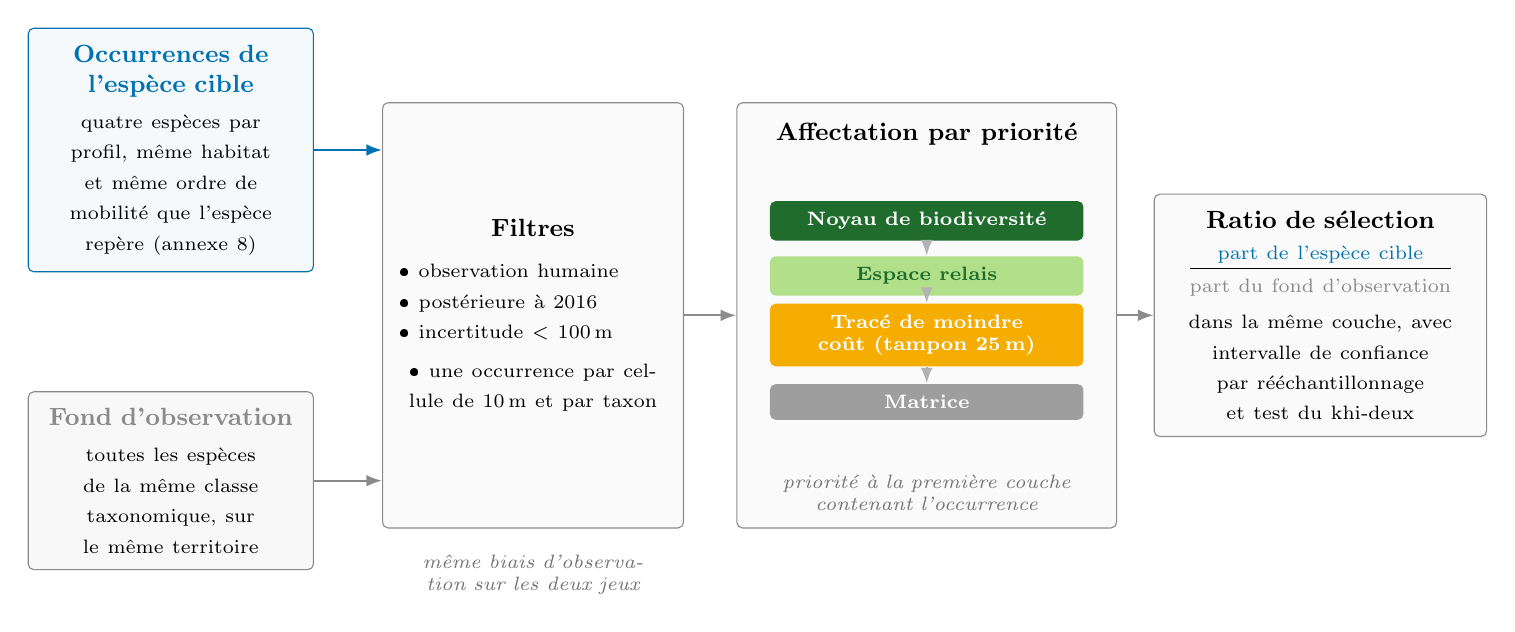
\begin{tikzpicture}[
  font=\small,
  boite/.style={draw, rounded corners=2pt, align=center, inner sep=6pt},
  source/.style={boite, text width=3.2cm},
  etape/.style={boite, draw=black!45, fill=black!2, text width=3.4cm},
  couche/.style={rounded corners=2pt, align=center, inner sep=4pt, text width=3.7cm,
                 font=\scriptsize\bfseries, text=white},
  fl/.style={-{Latex[length=2mm]}, black!45, thick},
]
% les deux jeux d'occurrences
\node[source, draw=cible, fill=cible!4] (cible) at (0,2.1)
  {\textbf{\textcolor{cible}{Occurrences de l'espèce cible}}\\[2pt]\scriptsize quatre espèces par profil, même habitat et même ordre de mobilité que l'espèce repère (annexe 8)};
\node[source, draw=fondobs, fill=fondobs!6] (fond) at (0,-2.1)
  {\textbf{\textcolor{fondobs}{Fond d'observation}}\\[2pt]\scriptsize toutes les espèces de la même classe taxonomique, sur le même territoire};
% les mêmes filtres pour les deux
\node[etape, minimum height=5.4cm] (filtres) at (4.6,0)
  {\textbf{Filtres}\\[7pt]\scriptsize\raggedright
   \textbullet~observation humaine\\[3pt]
   \textbullet~postérieure à 2016\\[3pt]
   \textbullet~incertitude \textless{} 100\,m\\[3pt]
   \textbullet~une occurrence par cellule de 10\,m et par taxon};
% affectation par priorité
\node[etape, text width=4.4cm, minimum height=5.4cm] (affect) at (9.6,0) {};
\node[anchor=north] at ([yshift=-4pt]affect.north) {\textbf{Affectation par priorité}};
\node[couche, fill=noyau] (c1) at (9.6,1.20) {Noyau de biodiversité};
\node[couche, fill=relais, text=noyau] (c2) at (9.6,0.50) {Espace relais};
\node[couche, fill=trace] (c3) at (9.6,-0.25) {Tracé de moindre coût (tampon 25\,m)};
\node[couche, fill=matrice] (c4) at (9.6,-1.10) {Matrice};
\draw[fl, black!30] (c1) -- (c2);\draw[fl, black!30] (c2) -- (c3);
\draw[fl, black!30] (c3) -- (c4);
\node[anchor=south, font=\scriptsize\itshape, text width=4.2cm,
       align=center, text=black!55] at ([yshift=3pt]affect.south)
  {priorité à la première couche contenant l'occurrence};
% le ratio
\node[etape, text width=3.8cm] (ratio) at (14.6,0)
  {\textbf{Ratio de sélection}\\[6pt]
   $\dfrac{\text{\scriptsize \textcolor{cible}{part de l'espèce cible}}}{\text{\scriptsize \textcolor{fondobs}{part du fond d'observation}}}$\\[6pt]
   \scriptsize dans la même couche, avec intervalle de confiance par rééchantillonnage et test du khi-deux};
% flux
\draw[fl, cible] (cible) -- (filtres.north west |- cible);
\draw[fl, fondobs] (fond) -- (filtres.south west |- fond);
\draw[fl] (filtres) -- (affect);
\draw[fl] (affect) -- (ratio);
\node[anchor=north, font=\scriptsize\itshape, text=black!55,
       text width=4.6cm, align=center] at ([yshift=-6pt]filtres.south)
  {même biais d'observation sur les deux jeux};
\end{tikzpicture}}
\caption{Protocole de confrontation aux occurrences GBIF : mêmes filtres et même affectation pour les espèces cibles et pour le fond d'observation, puis rapport des deux. Réalisation personnelle.}
\label{fig:schema-gbif}
\end{figure}

\chapter{Résultats}
Sur les six territoires et les quatre profils écologiques, la chaîne a produit vingt-quatre jeux de sorties de structure identique, exprimés dans la projection métrique locale et directement mobilisables en SIG comme dans le tableau de bord. Ce chapitre en présente les résultats : la connectivité par profil écologique (§3.1), sa variation entre territoires et le coût de calcul (§3.2), la sensibilité au paramétrage (§3.3), la confrontation aux occurrences d'espèces (§3.4) et l'effet d'un scénario d'aménagement (§3.5).

\section{Connectivité par profil écologique}
La part d'habitat fonctionnellement connecté, définie en §2.4.4, sert d'indicateur principal. Elle s'exprime entre 0 et 100 \%, ce qui la rend comparable entre des territoires d'emprises différentes, là où la surface connectée équivalente croît avec l'étendue. Le nombre de sous-réseaux, c'est-à-dire de sous-ensembles de taches toutes accessibles les unes aux autres, lui est complémentaire et indique en combien de morceaux séparés le réseau se découpe. La Table~3 donne, pour chaque profil écologique, la médiane et l'étendue de ces indicateurs sur les six territoires.
\begin{table}[H]
\centering
\small
\setlength{\tabcolsep}{5pt}
\caption{Récapitulatif des indicateurs par profil écologique, sur les six territoires : médiane et, entre crochets, étendue ; étendue seule pour le nombre de sous-réseaux.}
\begin{tabular}{@{}lllll@{}}
\toprule
\textbf{Profil} & \textbf{Habitat} & \textbf{Sous-} & \textbf{Tortuosité} & \textbf{Territoires à} \\
\textbf{écologique} & \textbf{connecté} & \textbf{réseaux} & \textbf{médiane} & \textbf{réseau connexe} \\
\midrule
Profil hérisson & 67 \% [40 à 83] & 1 à 2 & 1,61 [1,41 à 1,66] & 5 / 6 \\
Profil écureuil & 28 \% [17 à 82] & 1 à 11 & 1,38 [1,21 à 1,50] & 4 / 6 \\
Profil fauvette & 24 \% [15 à 69] & 1 à 28 & 1,34 [1,14 à 1,41] & 3 / 6 \\
Profil lézard & 23 \% [9 à 45] & 3 à 14 & 1,41 [1,39 à 1,47] & 0 / 6 \\
\bottomrule
\end{tabular}
\end{table}

Les valeurs obtenues s'étalent sur une plage étendue, d'un réseau presque intégralement connecté à un réseau très morcelé. Le profil hérisson est partout le mieux connecté : son réseau reste connexe dans cinq territoires sur six et sa part d'habitat connecté est la plus élevée (médiane 67 \%). Le profil lézard est à l'opposé : son réseau n'est jamais connexe (3 à 14 sous-réseaux) et sa part d'habitat connecté est la plus basse (médiane 23 \%). Les profils écureuil et fauvette sont intermédiaires, avec une forte variabilité entre territoires : le profil fauvette reste connexe à Nancy, à La Roche-sur-Yon et à Kourou, mais se fragmente en vingt-huit sous-réseaux à La Rochelle.

Perpignan, dont l'emprise compacte rend le contraste lisible, en donne un exemple concret (Figure~\ref{fig:sorties-perpignan}). Pour le profil hérisson, dont l'habitat couvre les milieux boisés, arbustifs et herbacés et dont la portée atteint trois kilomètres, les taches forment un ensemble unique dont tous les éléments sont accessibles les uns aux autres : 119 noyaux et 391 espaces relais, reliés par 1\,075 tracés de moindre coût, connectant 64 \% de l'habitat. Pour le profil lézard, dont l'habitat se limite aux milieux arbustifs, herbacés et aux sols nus et dont la portée n'excède pas 750 mètres, le même paysage se décompose en quatorze ensembles séparés, 91 noyaux et 514 espaces relais reliés par 1\,088 tracés, pour 23 \% d'habitat connecté. Le nombre de tracés est comparable d'un profil à l'autre : ce n'est pas le nombre de connexions qui distingue les deux réseaux mais leur agencement, les tracés du profil lézard reliant des groupes de taches voisines sans franchir les coupures qui séparent ces groupes, quand ceux du profil hérisson traversent tout le territoire.

\begin{figure}[H]
\centering
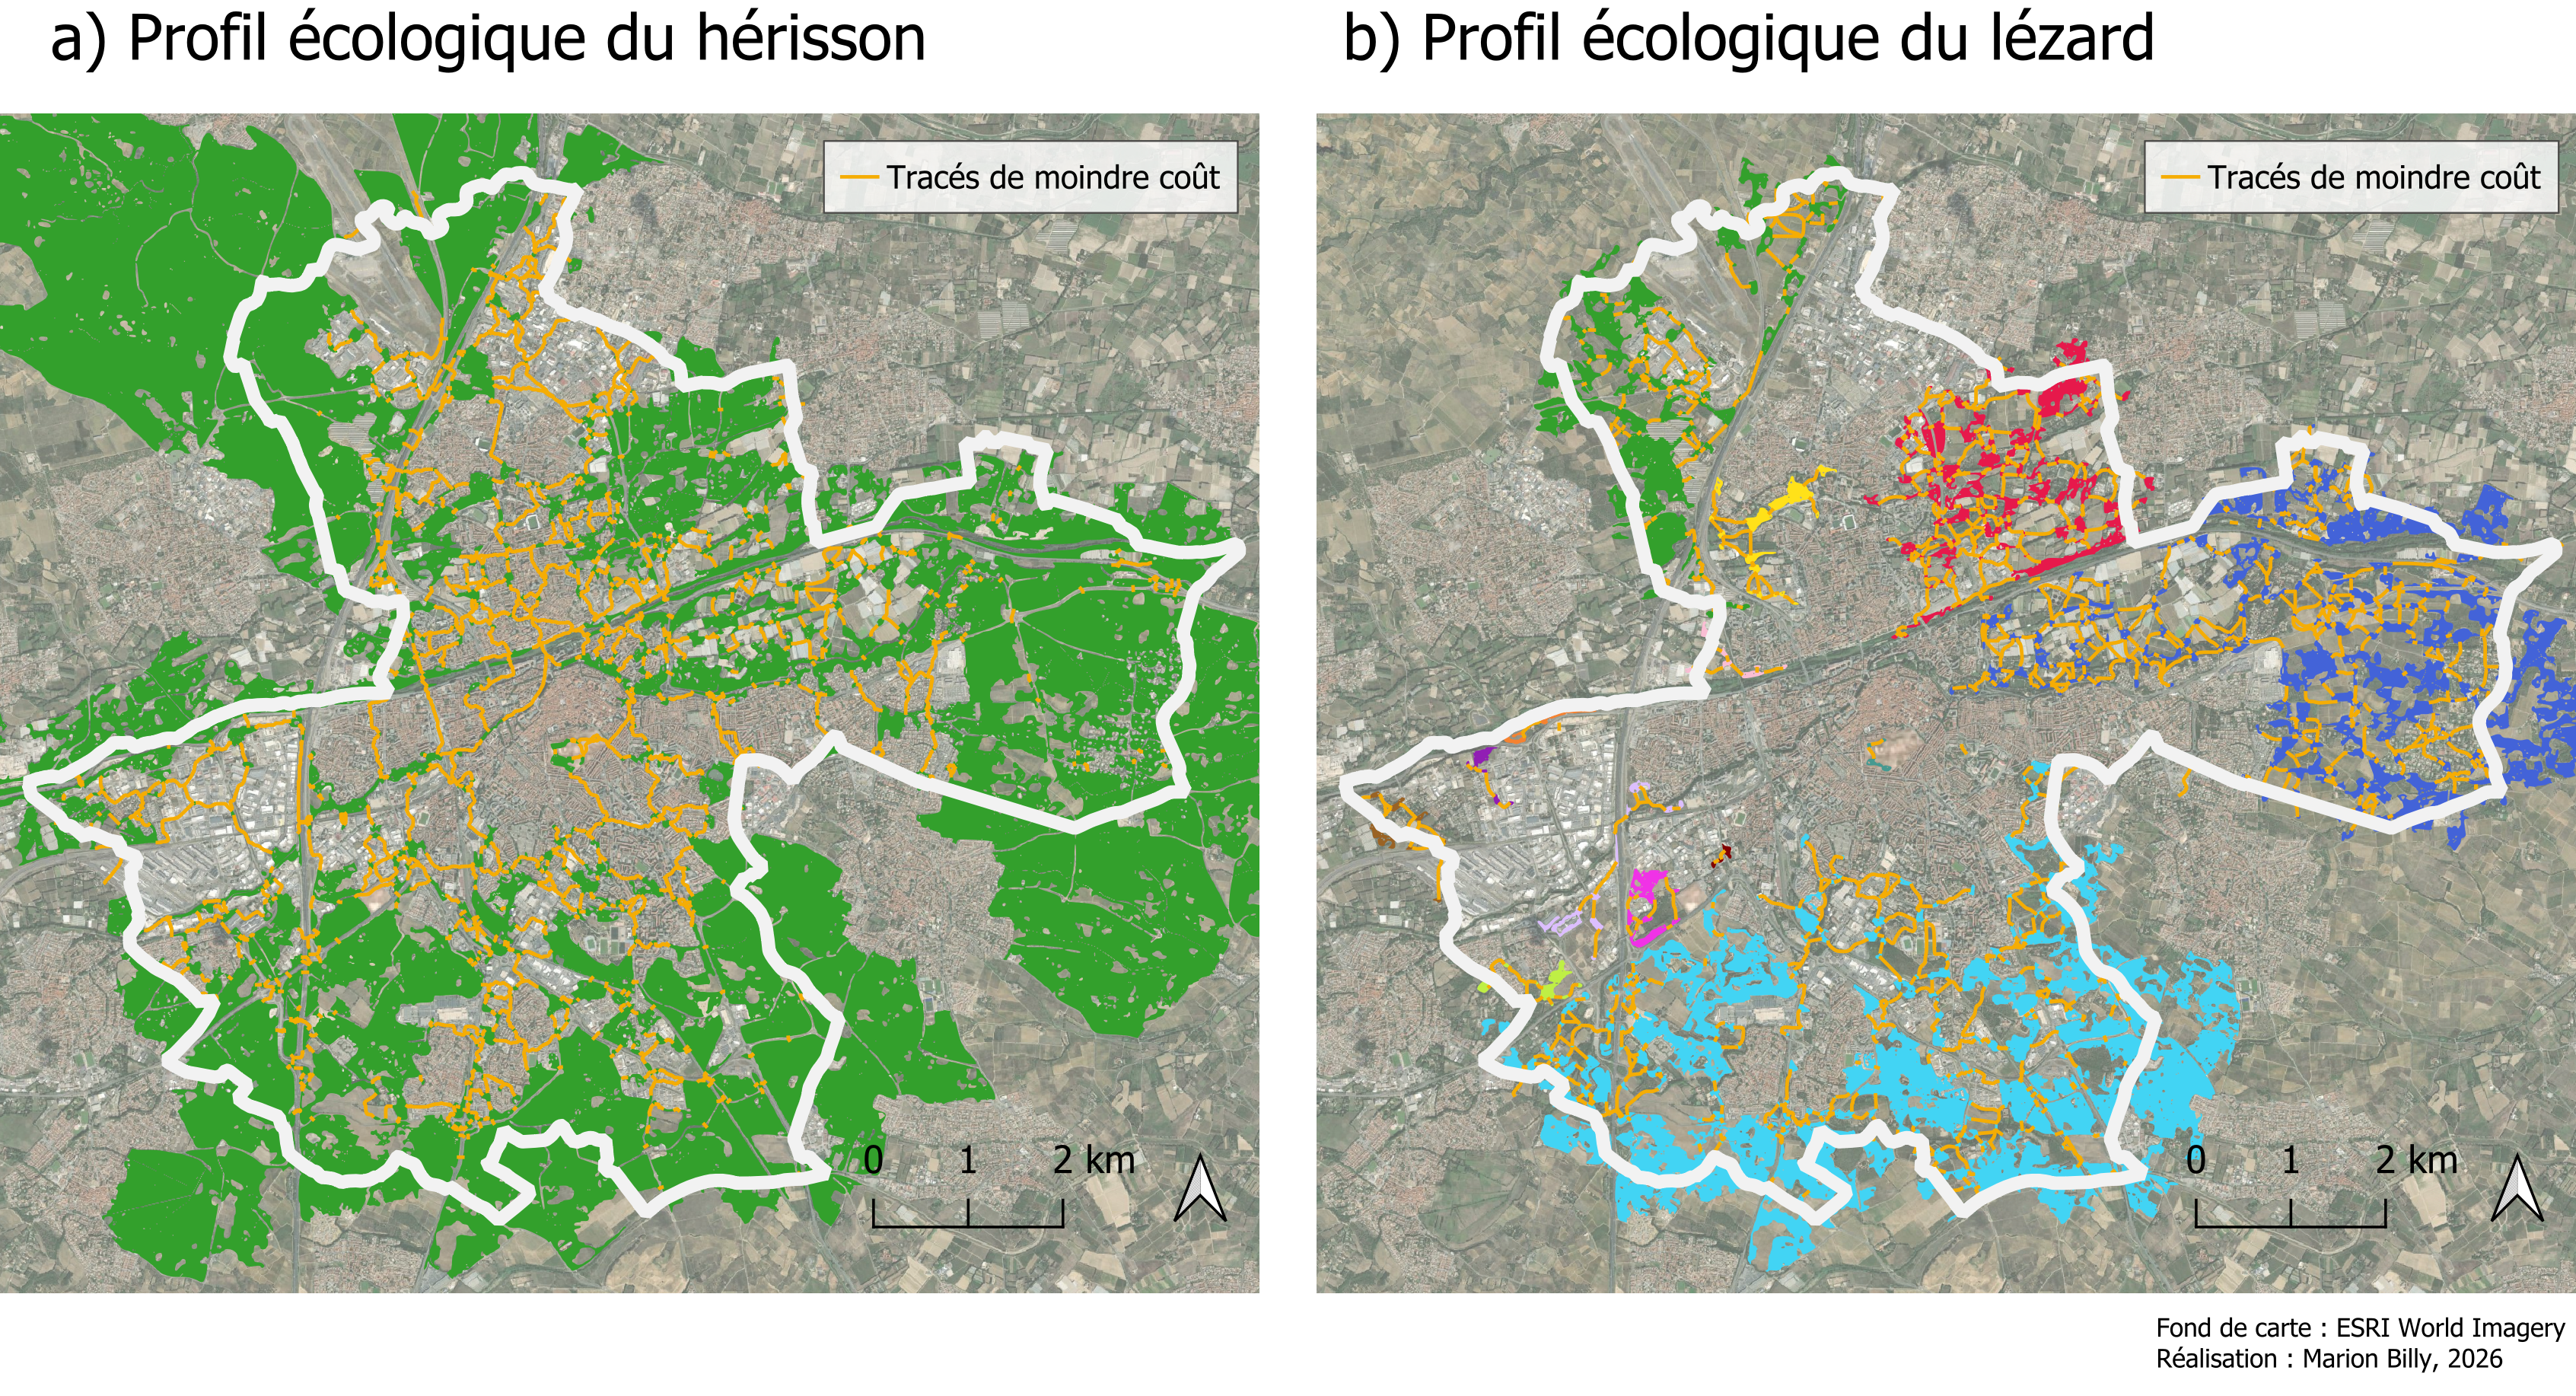
\includegraphics[width=\textwidth]{figures/subnetworks_perpi.png}
\caption{Sous-réseaux et tracés de moindre coût sur Perpignan : (a) profil hérisson, un unique ensemble relié ; (b) profil lézard, une couleur représente un sous-ensemble.}
\label{fig:sorties-perpignan}
\end{figure}

Les surfaces de dispersion rendent le même contraste visible (Figure~\ref{fig:dispersion}). Celle du profil hérisson couvre la quasi-totalité de la zone en restant loin de son budget de déplacement, ce que traduit un vert presque continu. Celle du profil lézard atteint vite sa limite de portée, l'orange et le rouge signalant un budget épuisé.

\begin{figure}[H]
\centering
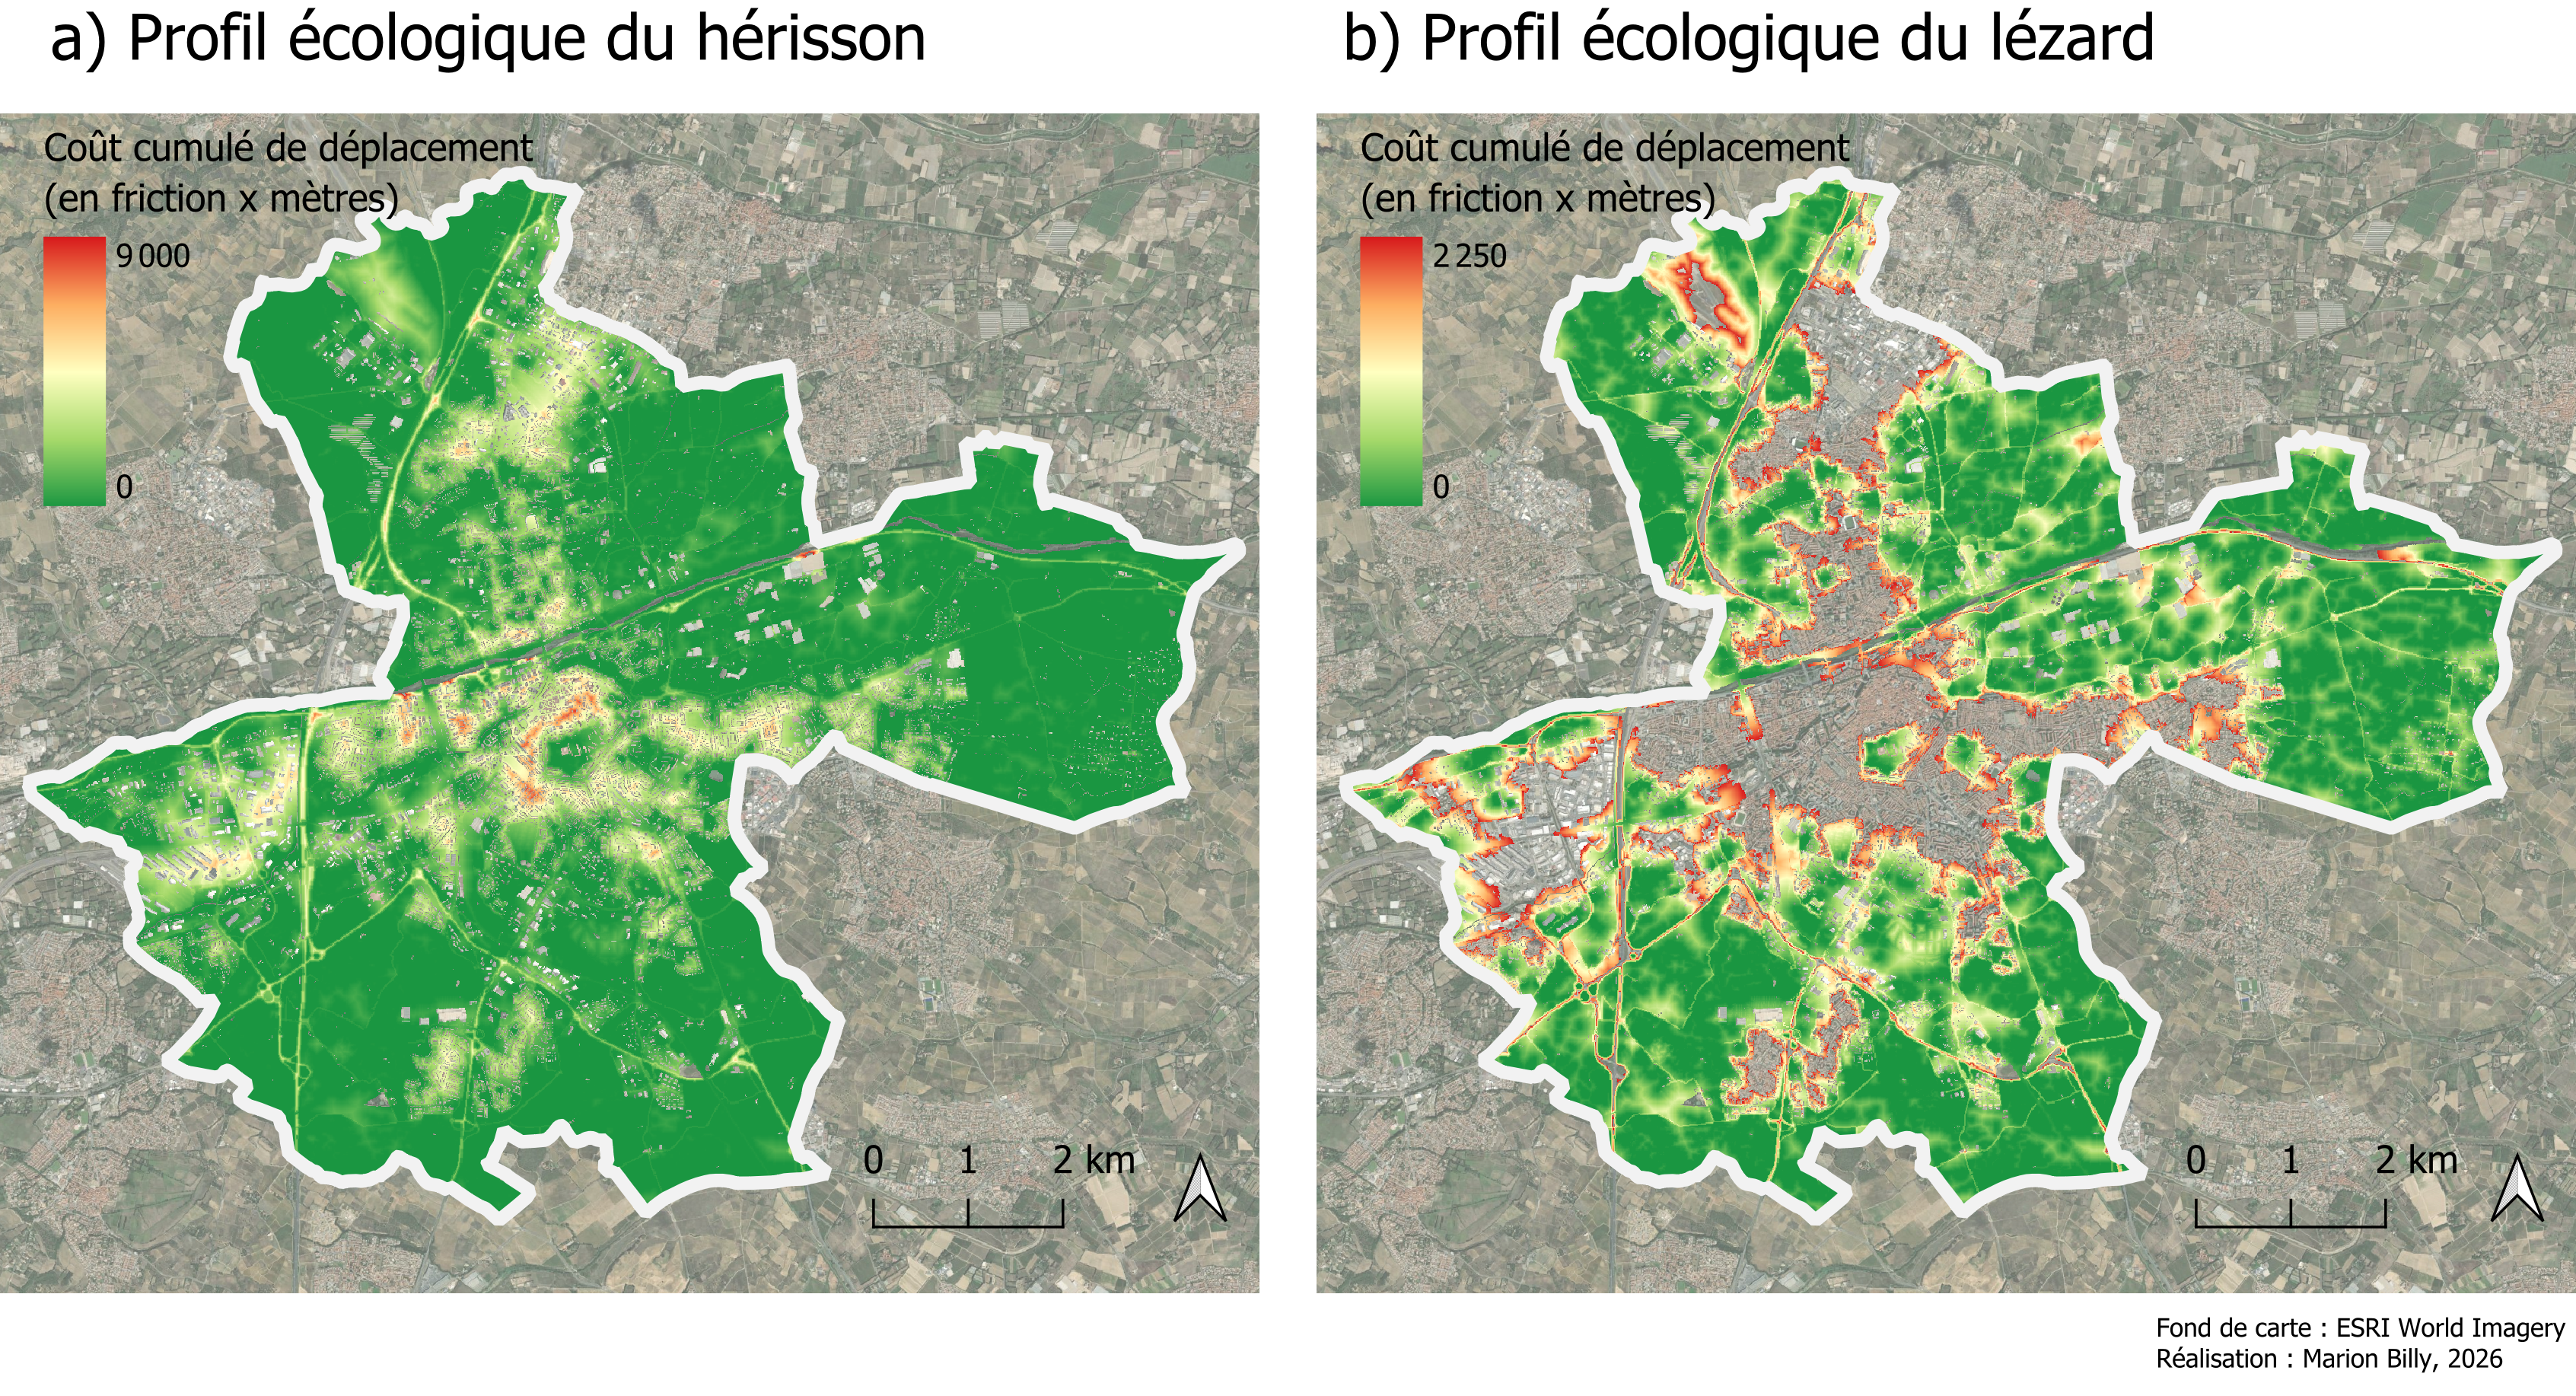
\includegraphics[width=\textwidth]{figures/dispersal_perpi.png}
\caption{Surfaces de dispersion comparées sur Perpignan : (a) profil hérisson, budget 9 000 ; (b) profil lézard, budget 2 250, d'où deux échelles distinctes. Vert : peu coûteux ; rouge : budget presque épuisé.}
\label{fig:dispersion}
\end{figure}

La tortuosité médiane des tracés complète cette lecture (Table~3). Elle rapporte la longueur du tracé de moindre coût à la distance à vol d'oiseau entre les deux taches : elle mesure le détour que le paysage impose au tracé, non la sinuosité d'une trajectoire réelle. Le profil hérisson, dont les liens sont longs et pour qui l'eau est infranchissable, supporte les détours les plus marqués, de 1,41 à 1,66 ; le profil fauvette, sans obstacle infranchissable, suit les tracés les plus directs, de 1,14 à 1,41. Ce détour modélisé ne prédit pas le comportement : l'écologie du mouvement rapporte des déplacements d'autant plus directs et rapides que la matrice est hostile, la sinuosité caractérisant plutôt la prospection au sein des milieux favorables (Sawyer et al., 2011 ; Balbi et al., 2019). Lue ainsi, une tortuosité élevée signale une contrainte du paysage, un réseau qui n'offre que des chemins détournés, et non une prédiction de trajectoire.

\section{Transposabilité entre territoires}
Appliquée à l'identique aux six territoires, sans aucun réglage propre à chaque site, la chaîne s'exécute intégralement sur chacun : une même commande produit le jeu de sorties complet sur des contextes bioclimatiques très différents. Cette transposabilité technique ne produit pas des résultats uniformes, et c'est ce qui fait sa valeur de diagnostic : la Table~4 rassemble les indicateurs des vingt-quatre couples territoire-profil.

\begin{table}[H]
\centering
\footnotesize
\setlength{\tabcolsep}{4pt}
\caption{Indicateurs de connectivité par territoire et par profil écologique : surface d'habitat et part de la zone d'étude, surface équivalente connectée (EC) et part de l'habitat connectée, tortuosité médiane des tracés, nombre de sous-réseaux. Territoires classés par part croissante d'arbres, arbustes et prairies.}
\begin{tabular}{@{}llrrrrrr@{}}
\toprule
 & & \multicolumn{1}{r}{\textbf{Habitat}} & & & & \multicolumn{1}{r}{\textbf{Tortuosité}} & \multicolumn{1}{r}{\textbf{Sous-}} \\
\textbf{Territoire} & \textbf{Profil} & \multicolumn{1}{r}{\textbf{(ha)}} & \multicolumn{1}{r}{\textbf{\% zone}} & \multicolumn{1}{r}{\textbf{EC (ha)}} & \multicolumn{1}{r}{\textbf{\% habitat}} & \multicolumn{1}{r}{\textbf{médiane}} & \multicolumn{1}{r}{\textbf{réseaux}} \\
\midrule
La Rochelle & Hérisson & 6\,556 & 19,8 & 2\,632 & 40,1 & 1,44 & 1 \\
 & Écureuil & 1\,479 & 4,5 & 253 & 17,1 & 1,31 & 11 \\
 & Fauvette & 1\,479 & 4,5 & 223 & 15,1 & 1,24 & 28 \\
 & Lézard & 4\,858 & 14,7 & 1\,627 & 33,5 & 1,47 & 14 \\
\addlinespace
Toulouse & Hérisson & 14\,891 & 32,3 & 7\,674 & 51,5 & 1,62 & 1 \\
 & Écureuil & 9\,161 & 19,9 & 2\,445 & 26,7 & 1,50 & 1 \\
 & Fauvette & 9\,161 & 19,9 & 1\,965 & 21,4 & 1,41 & 3 \\
 & Lézard & 5\,112 & 11,1 & 442 & 8,6 & 1,39 & 8 \\
\addlinespace
Perpignan & Hérisson & 2\,652 & 39,1 & 1\,707 & 64,4 & 1,61 & 1 \\
 & Écureuil & 753 & 11,1 & 209 & 27,7 & 1,37 & 3 \\
 & Fauvette & 1\,424 & 21,0 & 389 & 27,3 & 1,41 & 5 \\
 & Lézard & 1\,168 & 17,2 & 270 & 23,1 & 1,41 & 14 \\
\addlinespace
Nancy & Hérisson & 6\,926 & 48,5 & 4\,916 & 71,0 & 1,60 & 1 \\
 & Écureuil & 4\,735 & 33,1 & 2\,676 & 56,5 & 1,47 & 1 \\
 & Fauvette & 4\,735 & 33,1 & 2\,468 & 52,1 & 1,41 & 1 \\
 & Lézard & 2\,070 & 14,5 & 479 & 23,2 & 1,41 & 7 \\
\addlinespace
La Roche-sur-Yon & Hérisson & 25\,208 & 50,2 & 20\,864 & 82,8 & 1,66 & 1 \\
 & Écureuil & 9\,975 & 19,9 & 2\,747 & 27,5 & 1,38 & 1 \\
 & Fauvette & 9\,975 & 19,9 & 1\,932 & 19,4 & 1,27 & 1 \\
 & Lézard & 14\,349 & 28,6 & 2\,321 & 16,2 & 1,41 & 3 \\
\addlinespace
Kourou & Hérisson & 6\,458 & 52,7 & 4\,516 & 69,9 & 1,41 & 2 \\
 & Écureuil & 4\,565 & 37,2 & 3\,733 & 81,8 & 1,21 & 1 \\
 & Fauvette & 4\,565 & 37,2 & 3\,134 & 68,7 & 1,14 & 1 \\
 & Lézard & 1\,876 & 15,3 & 852 & 45,4 & 1,41 & 4 \\
\bottomrule
\end{tabular}
\end{table}

Pour un même profil, la part d'habitat connecté varie fortement d'un territoire à l'autre, de 40 \% à La Rochelle à 83 \% à La Roche-sur-Yon pour le profil hérisson. Le classement des territoires change selon le profil considéré, un territoire favorable au profil hérisson ne l'étant pas nécessairement pour les profils boisés ou thermophiles. En outre, aucun territoire ne connecte le profil lézard en un seul réseau.

La part végétalisée (arbres, arbustes, prairies) de chaque territoire ordonne largement ces résultats (Figure~\ref{fig:territoires-conn}). La Rochelle, la moins végétalisée (20 \% de couverture), est la plus fragmentée pour les profils boisés. Toulouse, métropole dense (32 \%), connecte encore bien le profil hérisson (52 \%) mais réduit le profil lézard à 9 \% de son habitat. Nancy et La Roche-sur-Yon, plus végétalisées (48 à 50 \%), conservent un réseau connexe pour le profil hérisson (71 et 83 \%). Une forte couverture végétale ne garantit toutefois pas la connectivité de chaque profil : La Roche-sur-Yon, verte à 50 \%, connecte 83 \% de l'habitat du profil hérisson mais 28 \% de celui du profil écureuil et 19 \% de celui du profil fauvette, l'habitat boisé y étant dispersé dans une matrice agricole.

\begin{figure}[H]
\centering
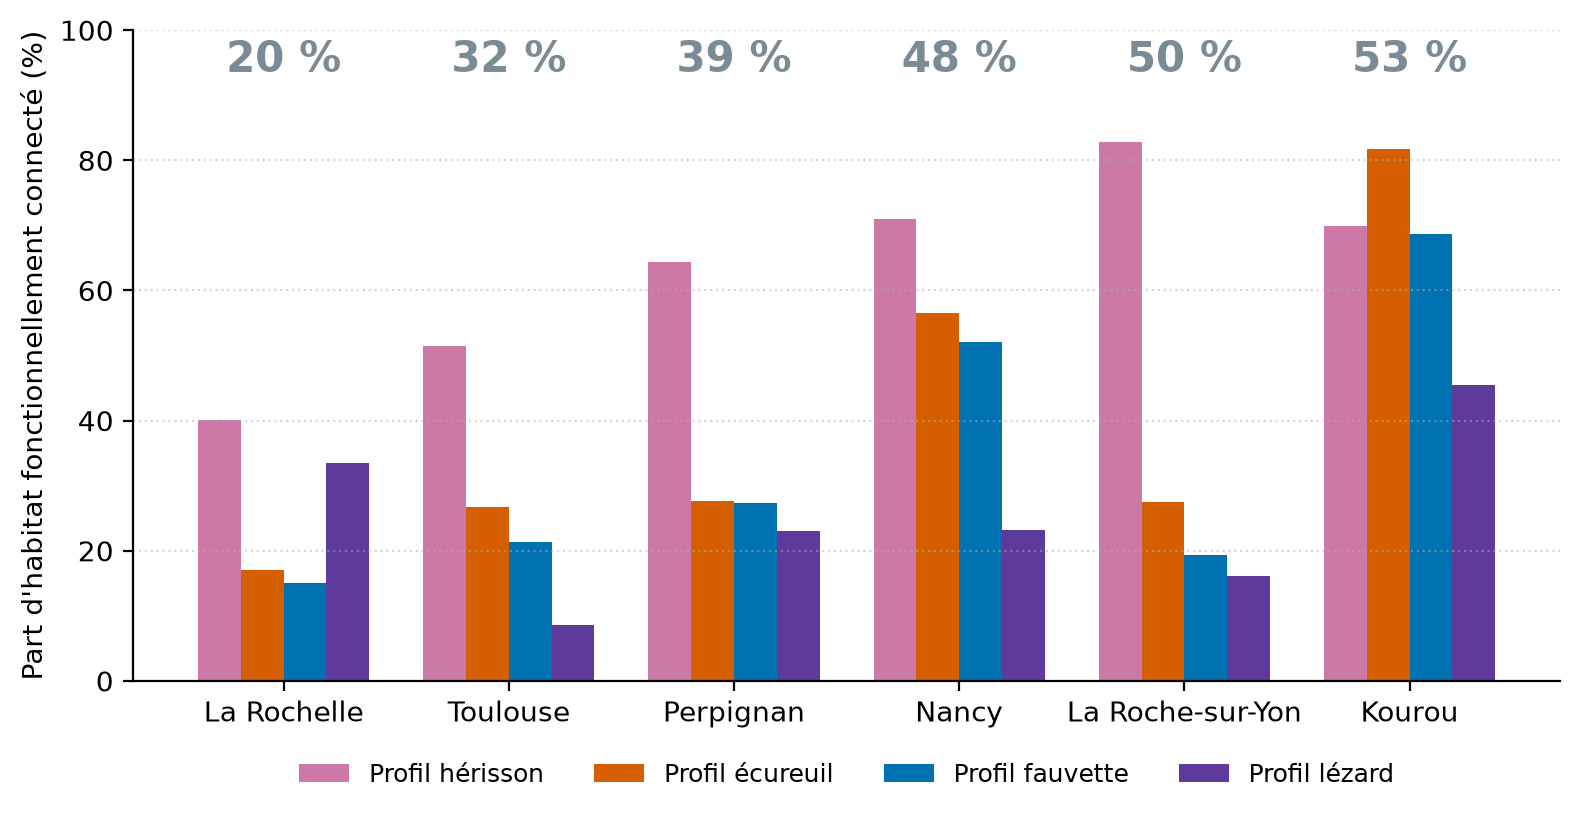
\includegraphics[width=\textwidth]{figures/territoire_connectivite.png}
\caption{Part d'habitat connecté par territoire et par profil écologique. Pourcentage au-dessus de chaque territoire : part de sa surface en arbres, arbustes ou prairies, qui ordonne les territoires.}
\label{fig:territoires-conn}
\end{figure}

Ce classement repose sur l'habitat du profil hérisson, le plus large des quatre, pris comme indicateur de végétalisation générale ; il ne coïncide pas avec l'habitat propre de chaque profil. Celui du reptile, milieux ouverts et sols nus, suit un ordre tout différent : La Roche-sur-Yon en compte 29 \% quand Toulouse, mieux classée sur l'axe, n'en a que 11 \%. La courbe du reptile ne suit donc pas la pente générale, non par irrégularité, mais parce que l'axe ne mesure pas son habitat.

La nature du couvert complète cette lecture. La Rochelle, littorale, est presque dépourvue de boisement (4,5 \% de forêt sur l'emprise), d'où la fragmentation des profils boisés. Toulouse conserve un couvert arboré modéré (20 \%) mais très peu de milieux ouverts (11 \%), d'où l'effondrement du profil lézard. Perpignan combine peu de forêt (11 \%) et une matrice arbustive, Nancy est le plus forestier des territoires tempérés (33 \%), et Kourou s'insère dans un couvert forestier équatorial (37 \%) : ses parts connectées, de 45 à 82 \% pour une couverture d'environ 53 \%, sont cohérentes avec une petite ville dans un couvert quasi continu, et ce territoire documente la transposabilité de la chaîne plutôt qu'un diagnostic exploitable.

La transposabilité se juge enfin au coût de calcul, qui conditionne l'industrialisation du service : une plateforme appelée à couvrir de nombreuses communes doit pouvoir exécuter des chemins de moindre coût sur chacune dans des délais tenables. La Table~5 donne la durée d'exécution complète des quatre profils par territoire, sur une machine virtuelle de 24 cœurs et 350 Go de mémoire vive (environnement en annexe 4, optimisations au §5.3).

\begin{table}[H]
\centering
\caption{Durée d'exécution complète des quatre profils écologiques par territoire, territoires classés par superficie croissante de la zone d'étude.}
\begin{tabularx}{\textwidth}{>{\raggedright\arraybackslash}X >{\raggedleft\arraybackslash}X >{\raggedleft\arraybackslash}X}
\toprule
\textbf{Territoire} & \textbf{Zone d'étude (km², tampon inclus)} & \textbf{Durée d'exécution (min)} \\
\midrule
Perpignan & 68 & 17 \\
Kourou (Guyane) & 123 & 8 \\
Nancy & 143 & 23 \\
La Rochelle & 331 & 35 \\
Toulouse & 461 & 156 \\
La Roche-sur-Yon & 502 & 116 \\
\bottomrule
\end{tabularx}
\end{table}

On remarque que la durée d'exécution n'est pas proportionnelle à la superficie du territoire : Kourou, deux fois plus étendu que Perpignan, s'exécute deux fois plus vite, et le traitement de Toulouse excède de quarente minutes celui de La Roche-sur-Yon sur une emprise plus petite. Ce qui détermine le coût est le nombre de taches d'habitat et de liens à tracer, donc la densité du réseau, et pas l'étendue du territoire. Le coût se concentre par ailleurs sur deux étapes : pour le couple le plus lourd, Toulouse et le profil hérisson à 86 minutes, le tracé des moindres coûts (environ 50 minutes) et la construction du graphe de Gabriel (environ 26 minutes) représentent à eux seuls près de neuf dixièmes du temps.

\section{Sensibilité au paramétrage}
Les deux dispositifs sont décrits en §2.7.1, ainsi que les indicateurs qui servent à juger de la stabilité des sorties, la part d'habitat connecté et le nombre de sous-réseaux ; les courbes de réponse et la synthèse par couple figurent en annexes 5 à 7.
 
Les balayages sur plage large délimitent d'abord le domaine de validité du diagnostic. Sur les plages parcourues, de 50 à 120 \% de la valeur de référence pour la distance de dispersion et de 0 à 200 \% pour le contraste de friction, la part d'habitat connecté est deux fois plus élevée aux valeurs les plus favorables du balayage qu'aux plus défavorables. Le nombre de sous-réseaux est bien plus sensible encore : celui du profil lézard à Toulouse, de huit en référence, atteint cent vingt-deux lorsque la distance de dispersion est ramenée à la moitié de sa valeur, et se réduit à un seul lorsque le contraste de friction est annulé. Aux valeurs extrêmes, ce n'est donc plus le même réseau qui est décrit : un habitat éclaté en une centaine de fragments isolés d'un côté, un territoire entièrement perméable de l'autre. Kourou fait exception : sa part connectée reste pratiquement constante sur tout le balayage de la distance de dispersion, alors qu'elle répond normalement au contraste de friction.
 
À l'intérieur de ce domaine, la perturbation locale montre un diagnostic stable au voisinage des valeurs retenues. Une erreur de 25 \% sur la distance de dispersion déplace la part d'habitat connecté de 5 à 14 \% selon le couple, et une erreur de 20 \% sur l'ensemble des frictions de 4 à 9 \%. Ces écarts sont du même ordre que l'imprécision attendue sur une calibration transposée d'un territoire à l'autre.
 
La hiérarchie des paramètres est le résultat le plus utile (Figure~\ref{fig:tornade}). Deux paramètres pilotent le diagnostic, la distance de dispersion et le contraste d'ensemble entre habitat et matrice. Le réglage classe par classe pèse près de dix fois moins, aucune classe ne déplaçant la part connectée de plus de 2,2 \%. Les plus influentes sont les chemins et la voirie secondaire, dont le coefficient conditionne la traversée du tissu résidentiel. Cinq classes n'ont au contraire aucun effet mesurable : les bâtiments et l'eau, parce qu'ils sont des obstacles pour ces deux profils et que leur coefficient est donc sans objet ; les zones humides, les mangroves et les sols nus, parce qu'ils sont trop peu présents dans l'emprise. L'effort de calibration doit donc porter sur ces deux paramètres plutôt que sur l'ajustement fin de chaque coefficient.
% [htbp] et non [H] : posée sur place, la figure ne tient pas dans les 7 cm que laisse
% le texte du §3.3 et laisse le bas de page blanc. En flottant, elle se pose en tête de
% la page suivante et le §3.4 remplit la page en cours.
\begin{figure}[htbp]
\centering
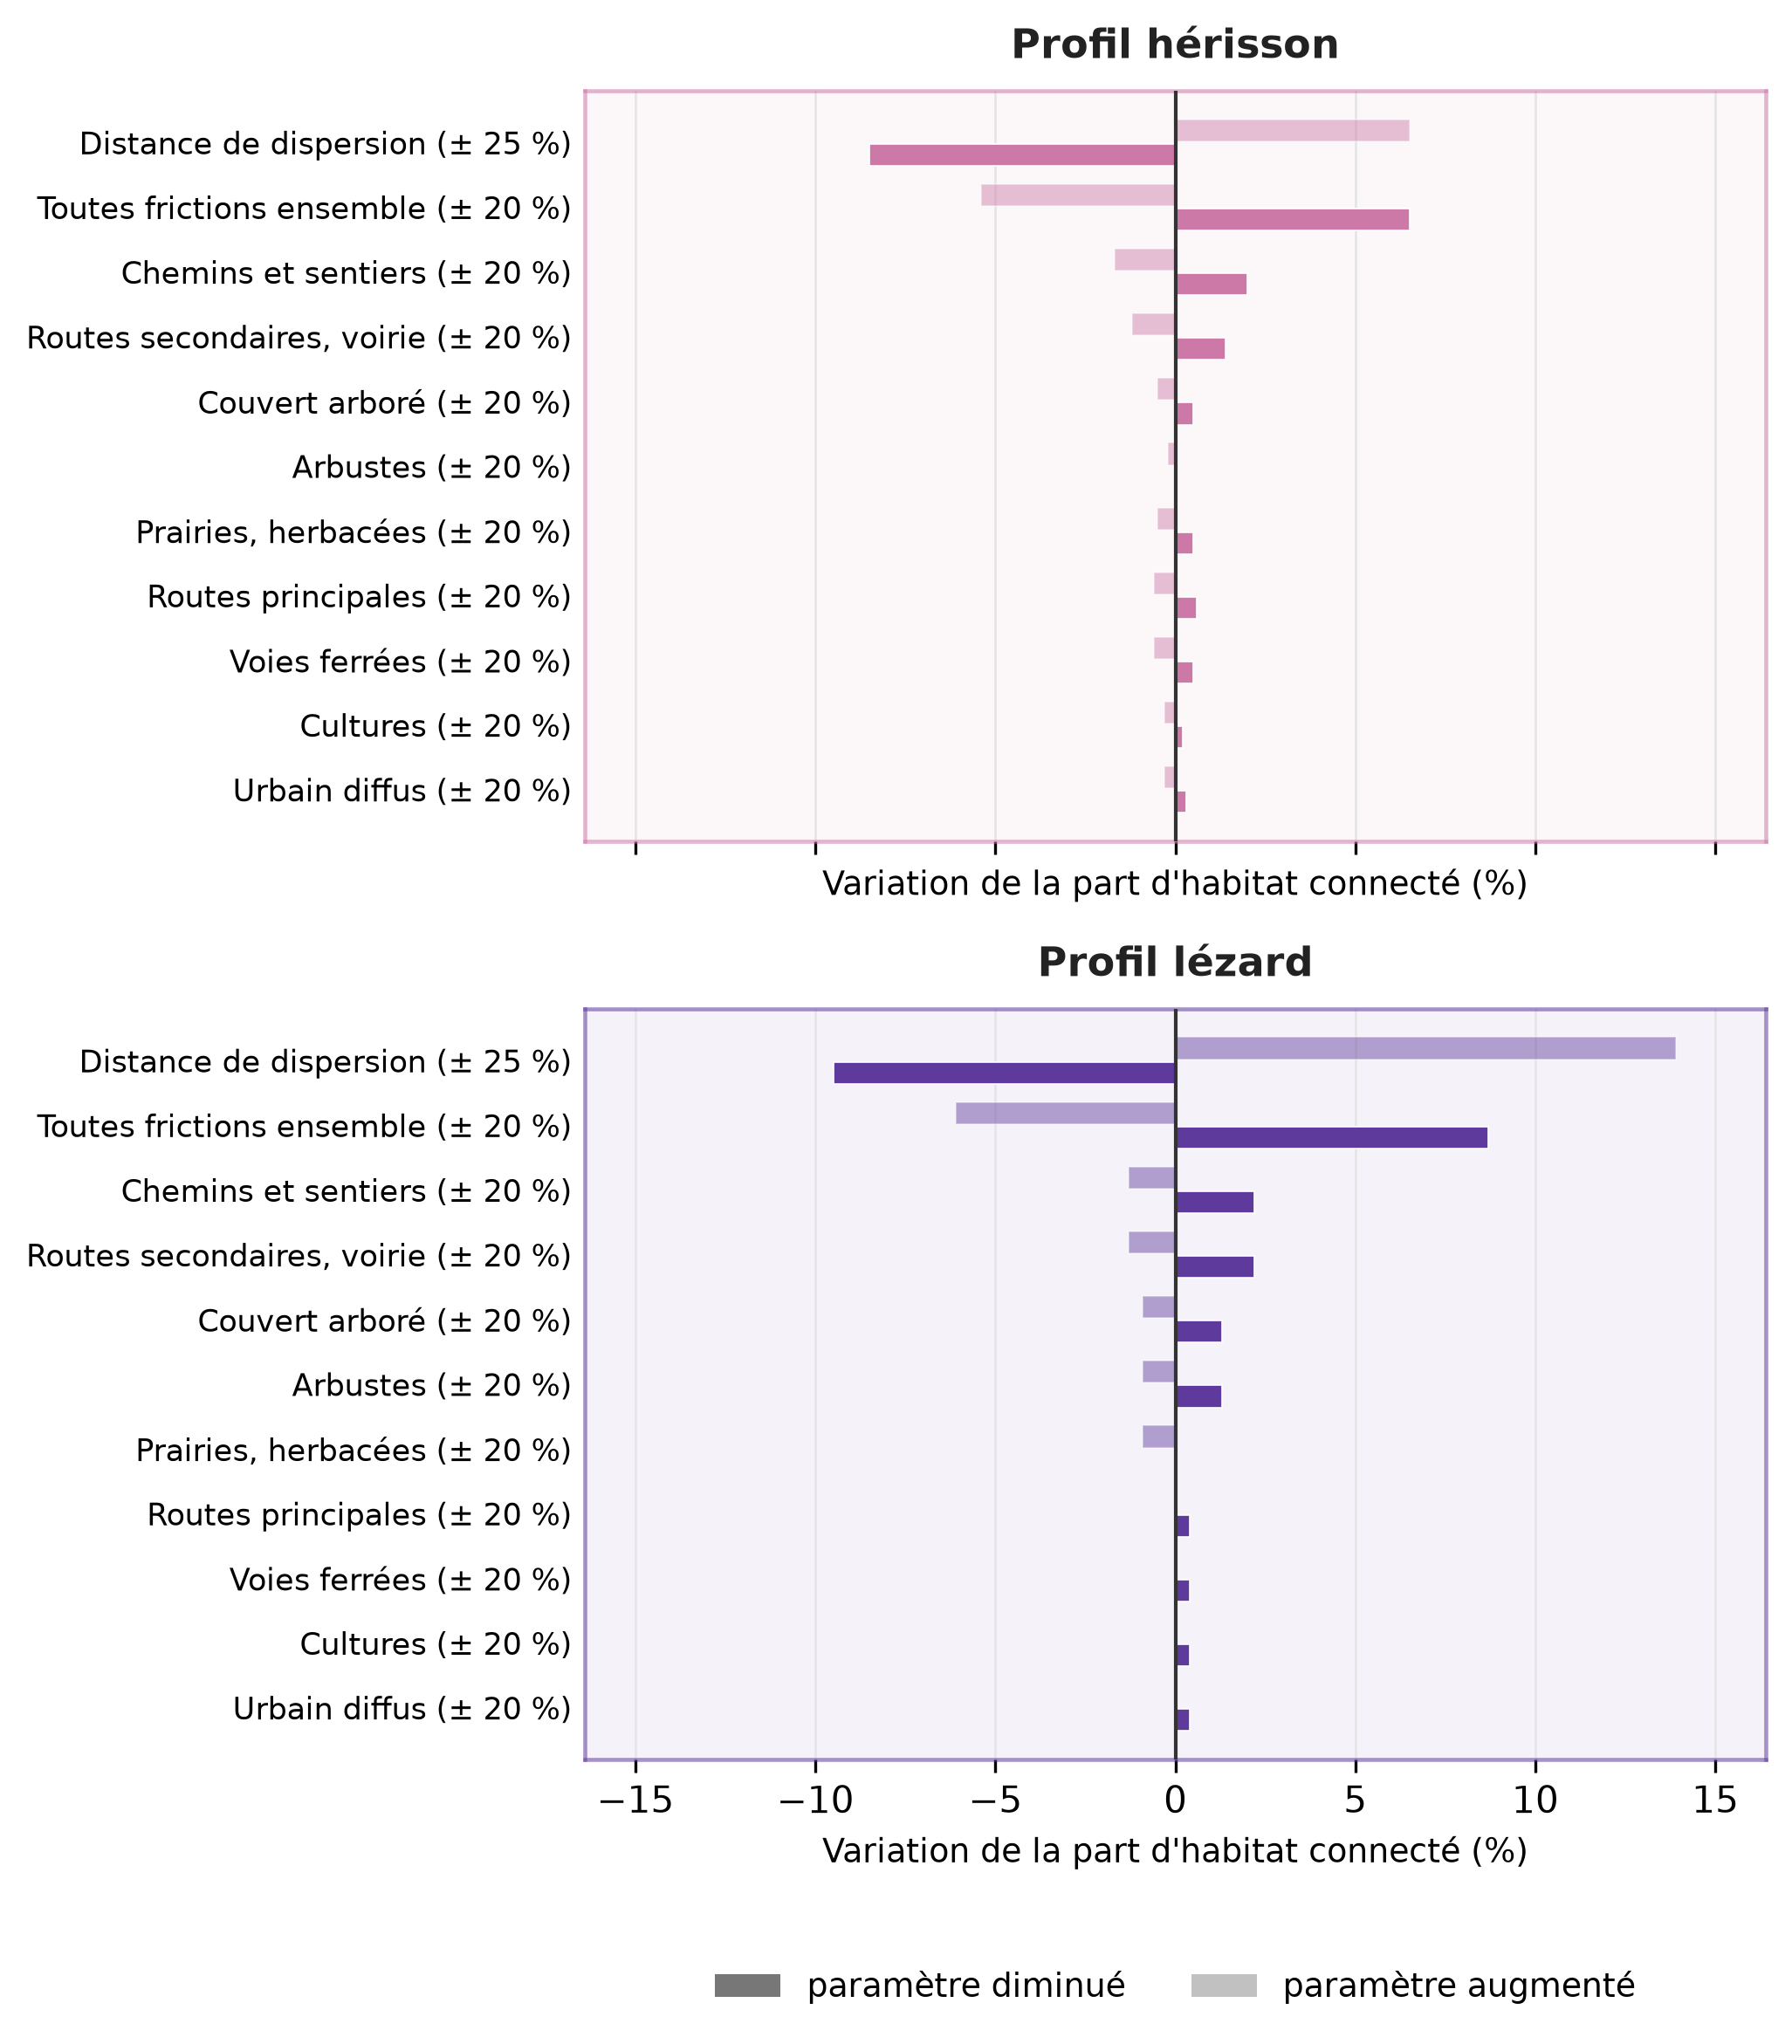
\includegraphics[width=0.92\textwidth]{figures/tornado_sensibilite.png}
\caption{Diagramme en tornade sur Perpignan : variation de la part d'habitat connecté sous perturbation des paramètres. Teinte pleine : paramètre diminué ; teinte claire : paramètre augmenté. Réalisation personnelle.}
\label{fig:tornade}
\end{figure}

\section{Confrontation aux occurrences d'espèces}
Le protocole est décrit en §2.7.2. Cette section en présente les ratios.

La confrontation porte sur 1\,567 occurrences, réparties en quatre espèces par profil écologique. Faute d'effectifs suffisants par territoire pour la plupart des profils, les ratios de sélection réunissent les occurrences des cinq territoires métropolitains (Figure~\ref{fig:gbif-ratios}, valeurs et intervalles de confiance en annexe 9 ; protocole en §2.7.2).

Les valeurs obtenues diffèrent nettement d'un profil à l'autre. Les deux profils d'habitat boisé sont trouvés dans les noyaux plus souvent que la répartition des observateurs ne l'expliquerait : le ratio atteint 1,80 pour le profil fauvette (994 occurrences) et 1,68 pour le profil écureuil (193 occurrences), avec des intervalles de confiance qui excluent la valeur de un dans les deux cas ; les espaces relais sont également sélectionnés par le profil fauvette (1,65), le ratio du profil écureuil (1,18) n'étant pas concluant. Symétriquement, ces deux profils sont sous-représentés dans la matrice (0,69 et 0,50) comme le long des tracés de moindre coût (0,76 et 0,64).

Le profil hérisson présente le schéma inverse. Ses occurrences sont sous-représentées dans les noyaux (0,39) et sur-représentées le long des tracés de moindre coût (1,74) comme dans la matrice (1,45), sur 89 occurrences retenues ; le ratio des espaces relais (1,92) va dans le même sens, mais son intervalle de confiance (0,96 à 3,04) inclut la valeur de un.

Le profil lézard ne produit pas de signal d'ensemble : ses ratios noyau (0,86), tracé (1,19) et matrice (1,00) ont des intervalles de confiance qui englobent la valeur de un, et seul le ratio des espaces relais (0,50, intervalle 0,17 à 0,92) s'en écarte, sur six occurrences seulement.

\begin{figure}[H]
\centering
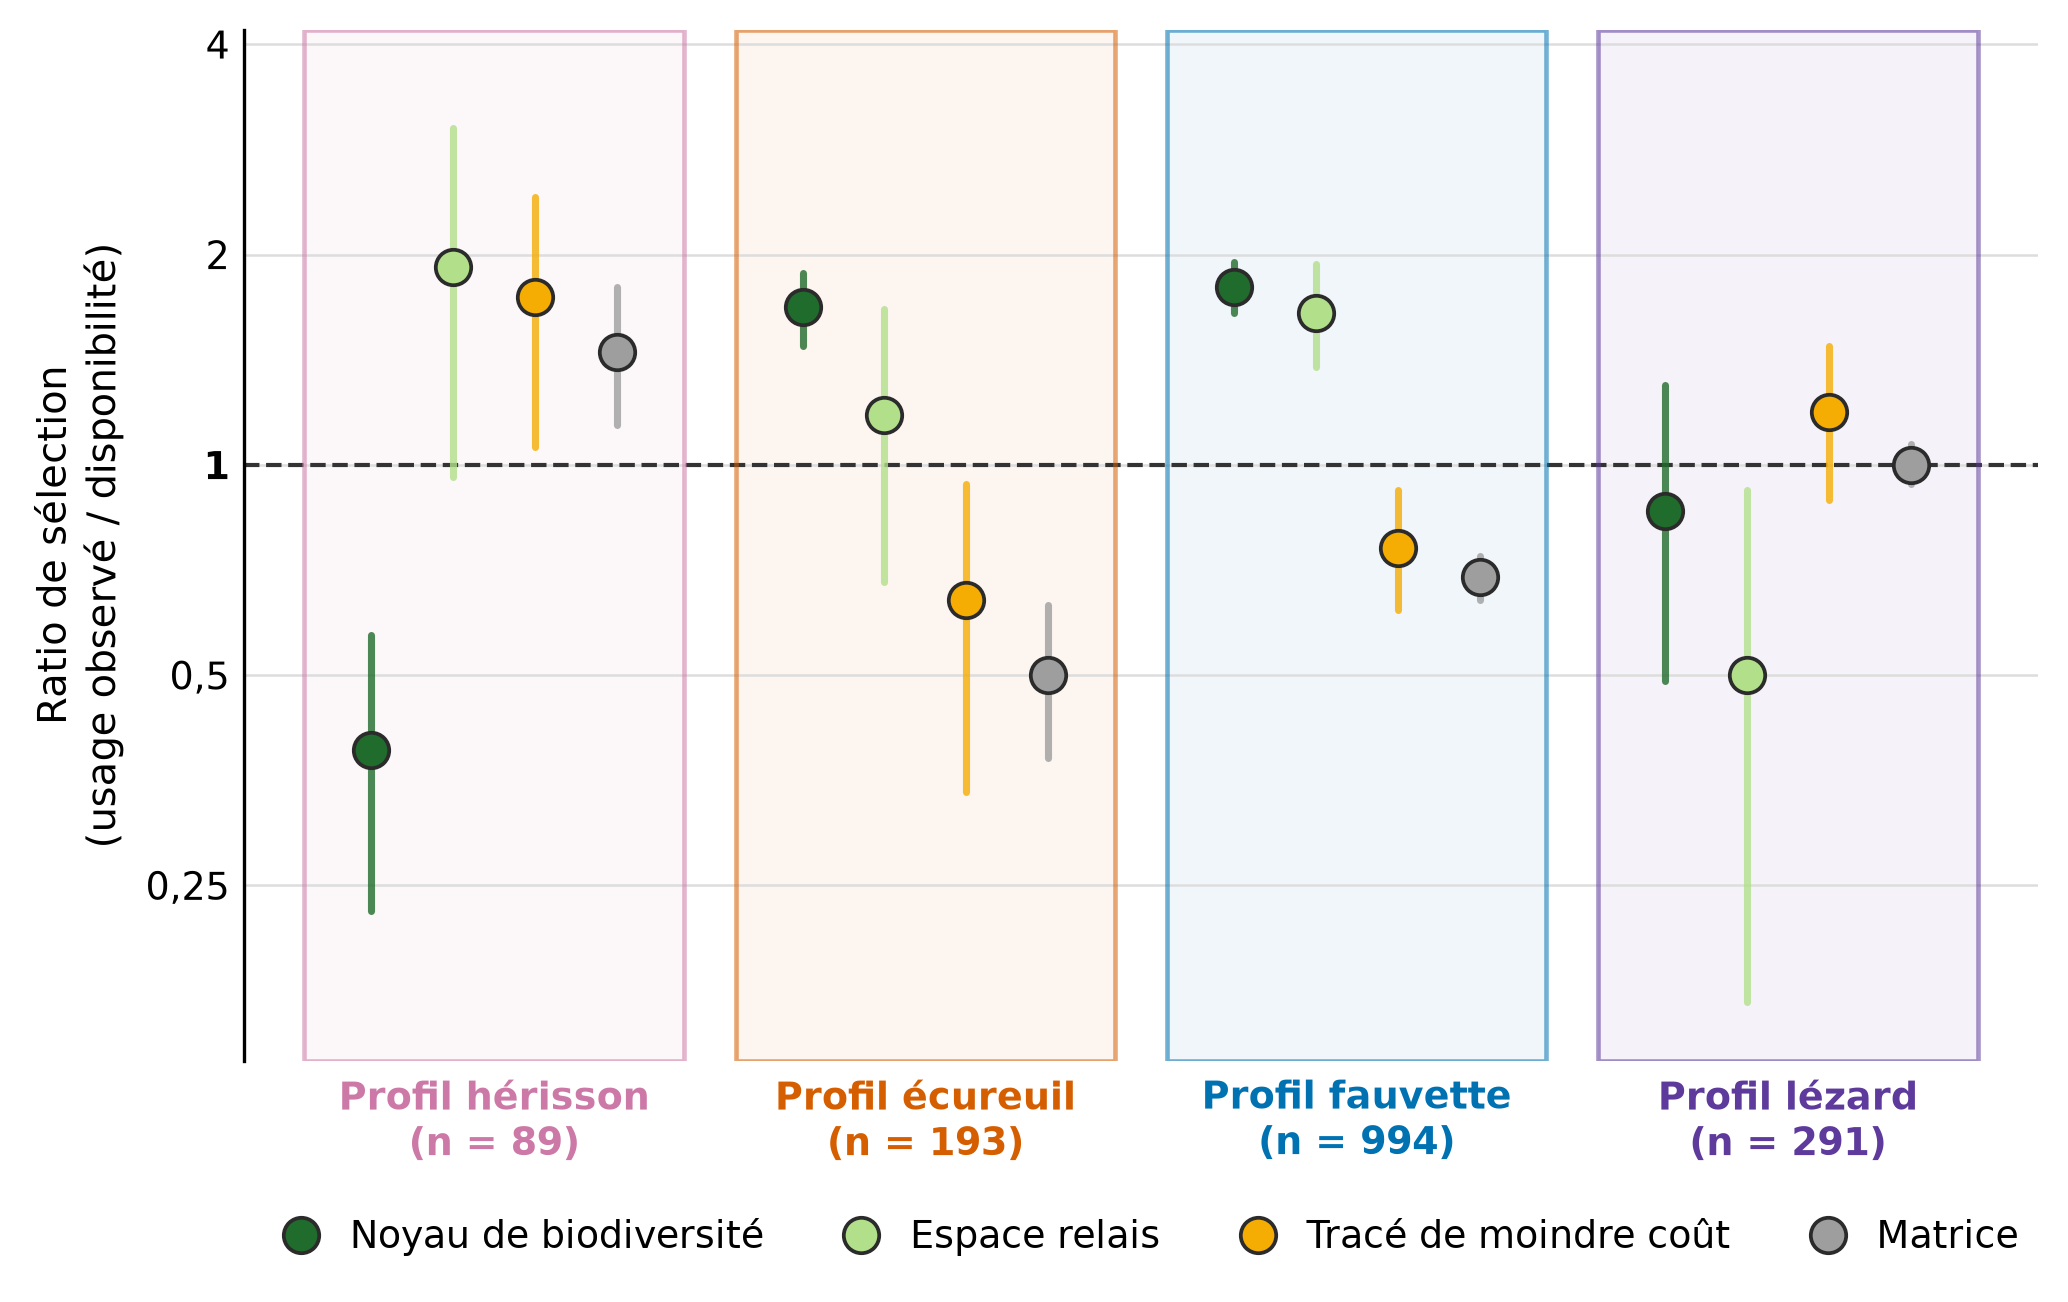
\includegraphics[width=\textwidth]{figures/gbif_ratios_pooled.png}
\caption{Ratios de sélection GBIF par profil et par classe d'espace, agrégés sur les cinq territoires tempérés. Moustaches : intervalle de confiance à 95 \% ; axe vertical logarithmique. Réalisation personnelle d'après les données GBIF (2026)}
\label{fig:gbif-ratios}
\end{figure}

Le test du khi-deux confirme cette lecture (annexe 10). L'écart à une répartition indifférente est hautement significatif pour les profils fauvette, écureuil et hérisson, avec des valeurs de p inférieures à $10^{-5}$, et non significatif pour le profil lézard (p = 0,21), dont la répartition est indiscernable de celle du fond d'observation.

La couverture est très inégale selon le profil et le territoire (annexe 8). Toulouse fournit à elle seule la majeure partie des occurrences, avec 710 des 994 du profil fauvette et 222 des 291 du profil lézard, c'est la seule ville à réunir un effectif exploitable pour les quatre profils. Quatre couples territoire-profil comptent moins de cinq occurrences, effectif trop faible pour une lecture isolée. La répartition spatiale des occurrences est cartographiée pour le profil fauvette à Toulouse (Figure~\ref{fig:gbif-toulouse}).


\begin{figure}[H]
\centering
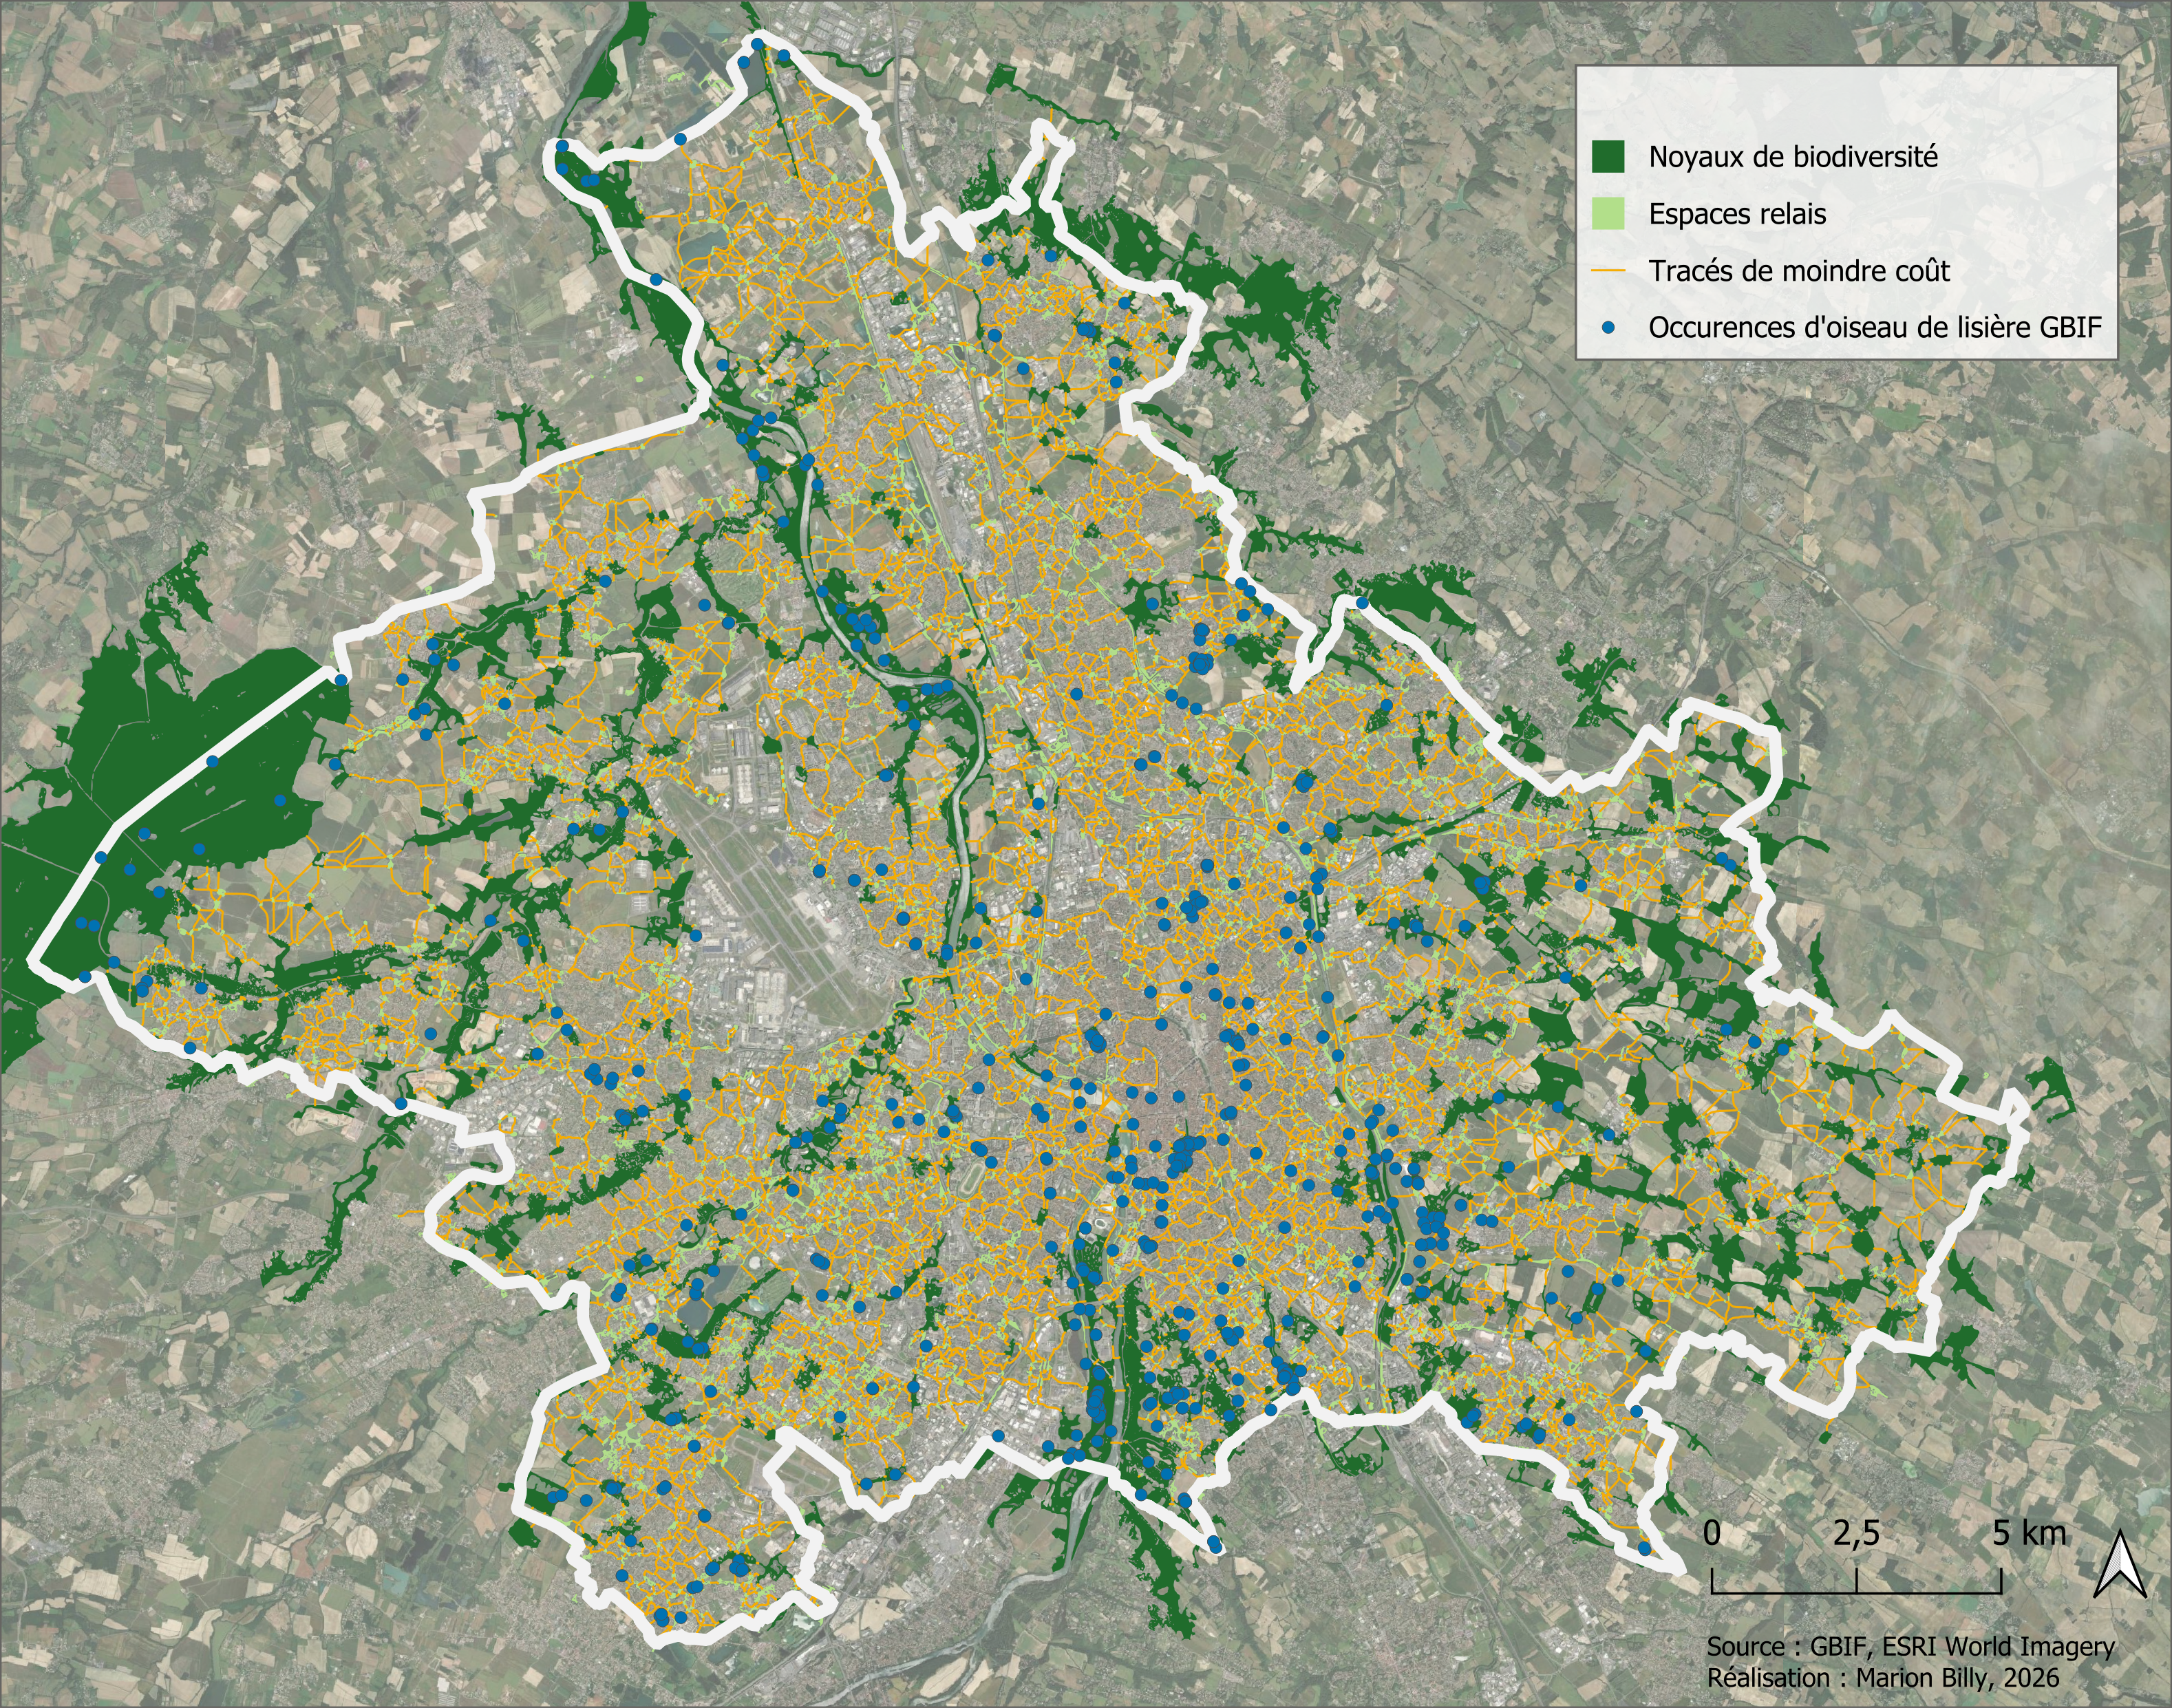
\includegraphics[width=\textwidth]{figures/gbif_fauvette_toulouse.png}
\caption{Occurrences GBIF du profil fauvette à Toulouse, sur les noyaux de biodiversité, les espaces relais et les tracés de moindre coût. (d'après les données GBIF, 2026)}
\label{fig:gbif-toulouse}
\end{figure}

\section{Effet local d'un scénario de végétalisation à Toulouse}
Au-delà du diagnostic de l'état existant, la chaîne estime l'effet attendu d'un projet d'aménagement sur la connectivité, avant sa réalisation, en comparant deux états à indicateurs identiques : le projet est intégré à l'occupation du sol comme une modification locale, puis la chaîne est relancée sur l'état modifié et ses sorties sont comparées à celles de l'état initial.

Ce mécanisme est illustré par une végétalisation arbustive de près de cinq hectares à Toulouse, le long des ramblas des allées Jean-Jaurès. Pour le profil fauvette (Figure~\ref{fig:scenario}), l'emprise végétalisée dépasse le seuil de cœur compact et s'ajoute aux noyaux de la zone d'étude, qui passent de 404 à 405. L'étape de moindre coût la raccorde alors à ses voisins en créant quatre tracés de moindre coût. Une liaison directe entre deux espaces relais voisins n'apparaît plus après l'aménagement : le nouveau noyau s'interposant entre eux, le critère de Gabriel (§2.4.2) remplace la liaison directe par deux liaisons passant par lui. Le site devient un point d'appui pour la circulation locale et étend le réseau. À l'échelle du territoire en revanche, les indicateurs agrégés sont inchangés : la surface connectée équivalente du profil reste à 1 964,8 hectares, la part d'habitat connecté à 21,4 \% et le nombre de sous-réseaux à trois. Le constat vaut pour les quatre profils, dont aucun indicateur agrégé ne varie de plus de 0,1 \% ; celui du profil hérisson, le plus mobile, passe de 7 674,2 à 7 674,6 hectares de surface connectée équivalente.

\begin{figure}[H]
\centering
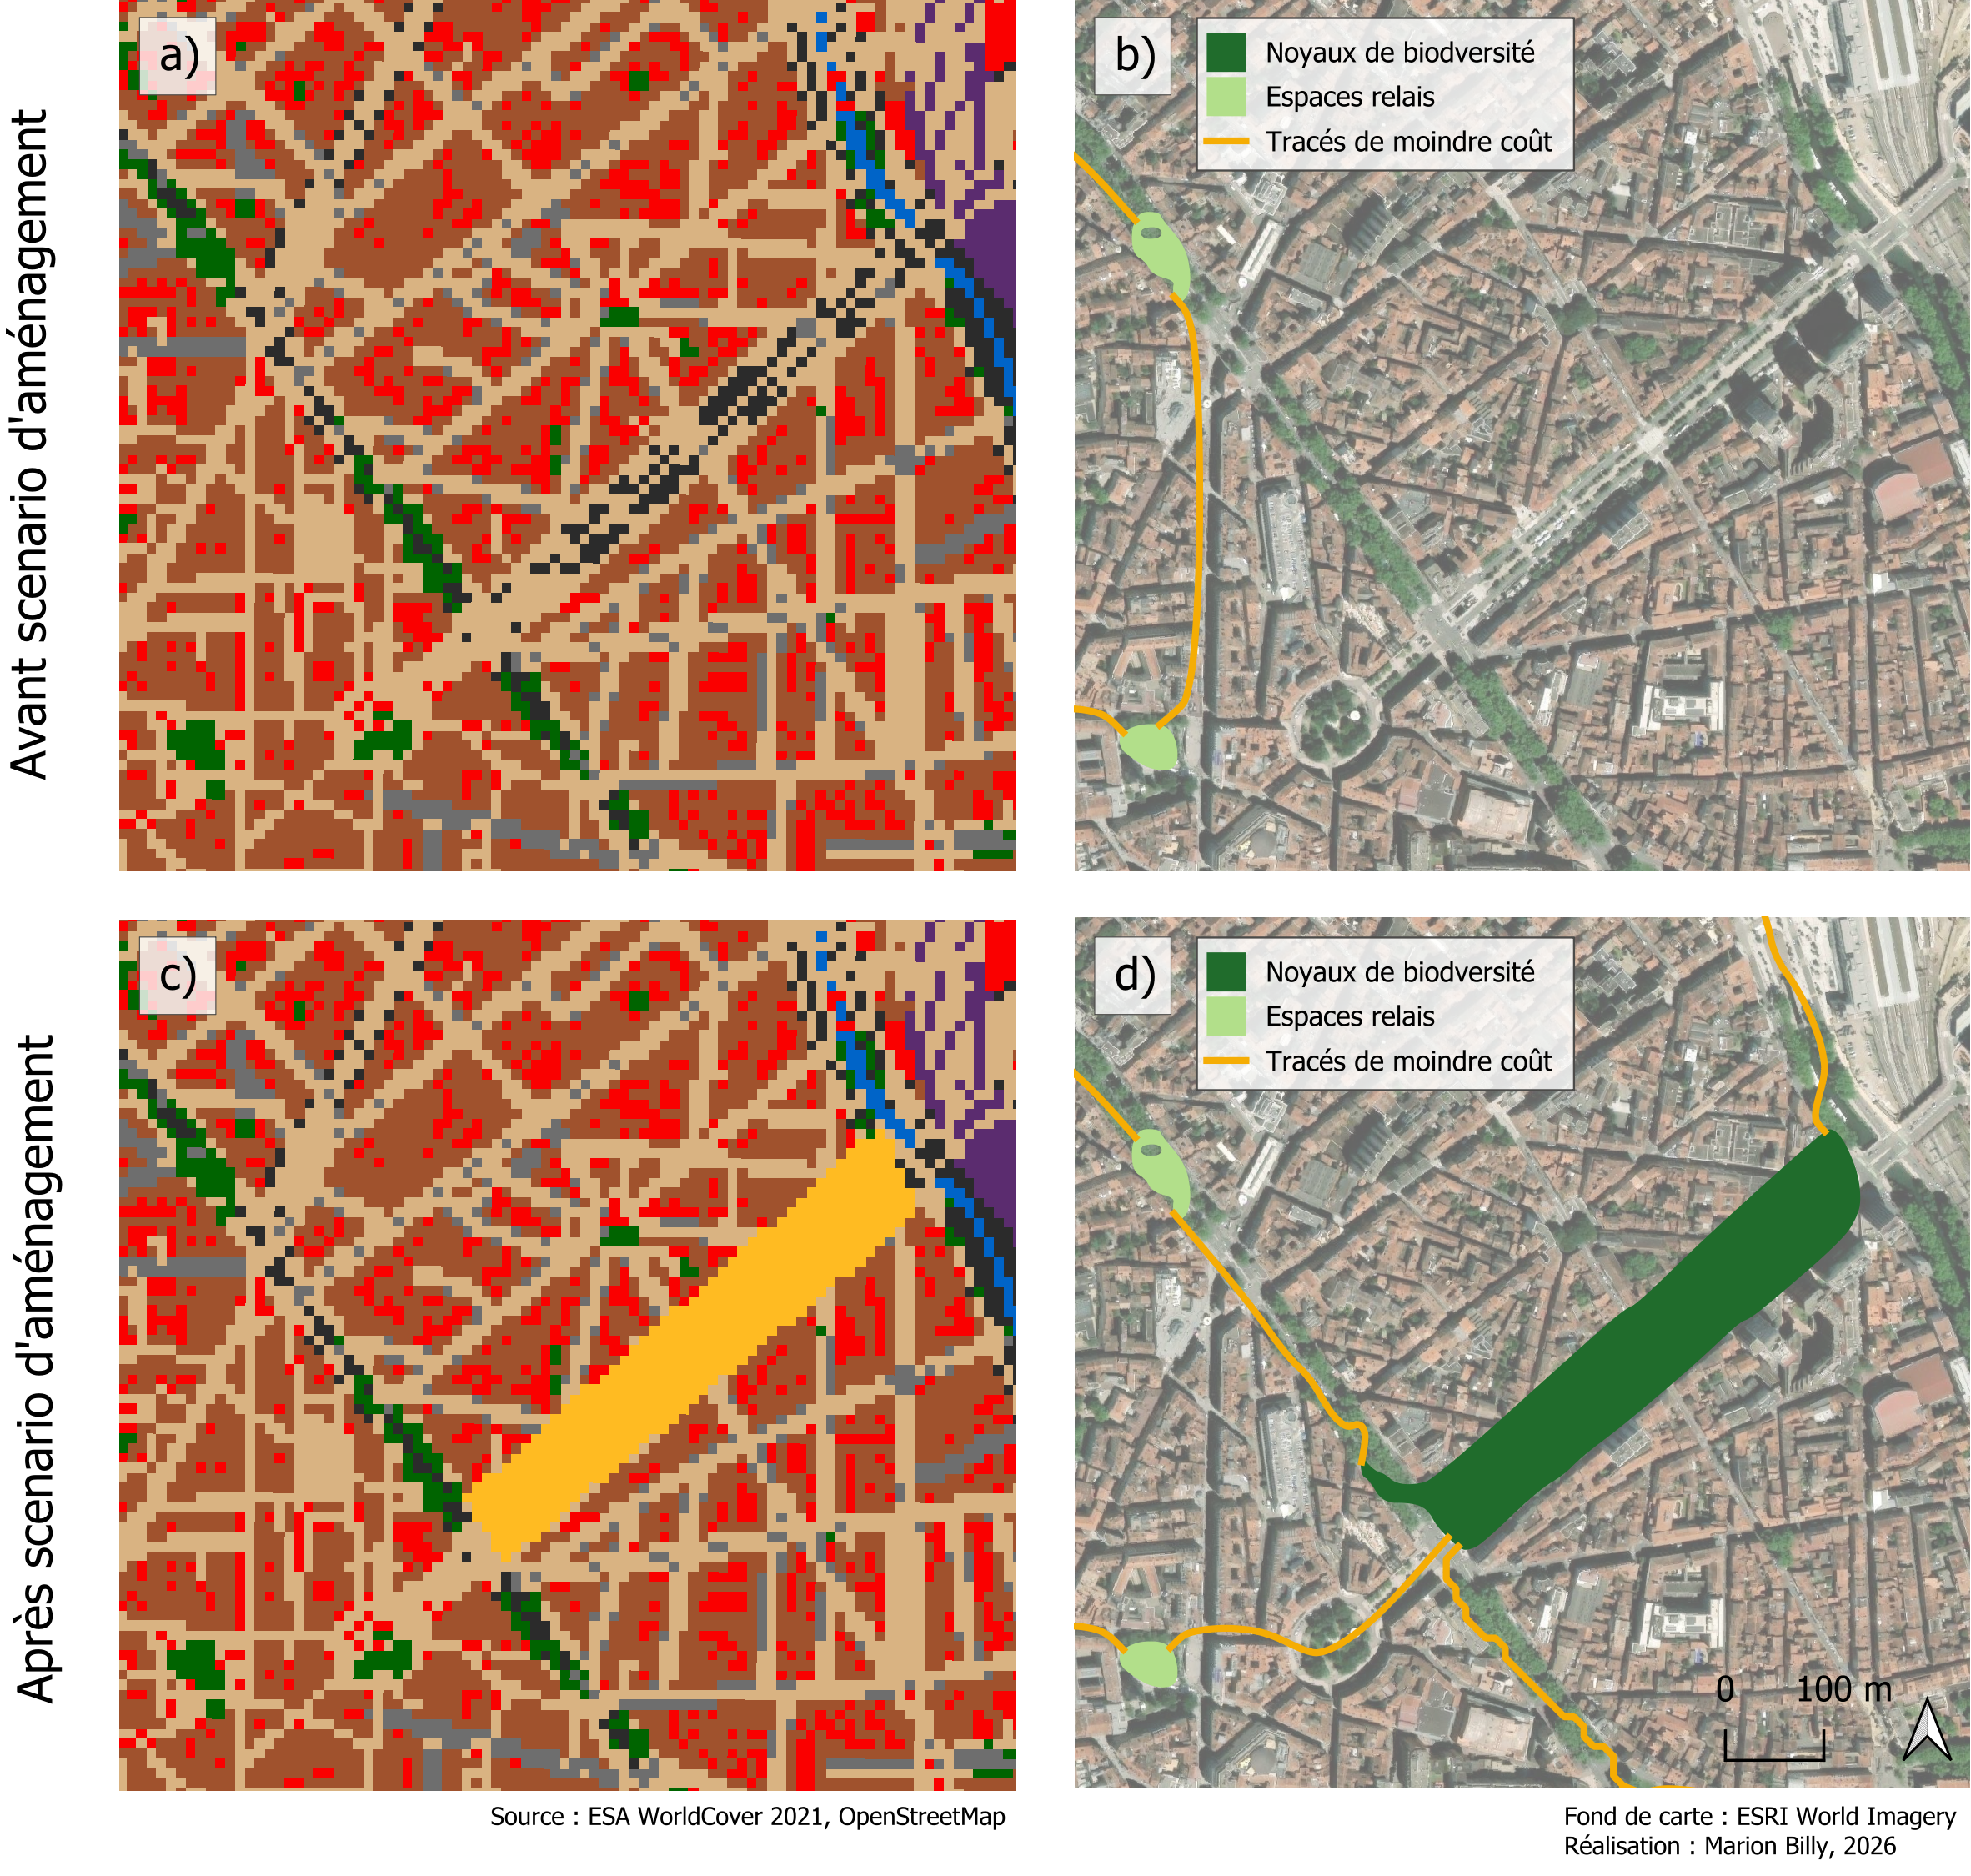
\includegraphics[width=\textwidth]{figures/scenario_jj_fauvette.png}
\caption{Scénario de végétalisation des allées Jean-Jaurès à Toulouse, profil fauvette. Occupation du sol enrichie avant (a) et après (c) intégration du projet ; noyaux de biodiversité, espaces relais et tracés de moindre coût correspondant (b, d).}
\label{fig:scenario}
\end{figure}

\chapter{Discussion}
La section 4.1 examine ce qui fait varier la connectivité mesurée, selon le profil écologique considéré, selon le territoire et selon l'échelle à laquelle elle est lue. La section 4.2 précise la portée de ces résultats et la confiance qu'ils autorisent. La section 4.3 expose les limites de l'approche et les remèdes qu'elles appellent. La section 4.4 en tire le positionnement opérationnel de l'outil et son domaine d'emploi.

\section{Une connectivité relative : profils, territoires, échelles de lecture}
\subsection{Des réseaux distincts selon le profil écologique}
Les résultats montrent d'abord que la connectivité d'un même territoire diffère nettement selon le profil écologique considéré. Restaurer la connectivité pour le profil hérisson, qui dispose d'une large capacité de déplacement mais pour qui les cours d'eau font obstacle, n'a pas le même sens que pour le profil lézard, dont l'habitat thermophile est dispersé et qui se déplace peu. En restituant quatre réseaux distincts pour un même territoire, l'outil explicite cette multiplicité et conduit à préciser pour quel profil la connectivité est évaluée. Cette lecture par profil ne se transpose pas directement dans un document d'urbanisme, organisé par sous-trames nationales, c'est-à-dire par type de milieu et non par capacité de déplacement. Une correspondance est possible, les profils écureuil et fauvette vers la sous-trame boisée, profil lézard vers les milieux ouverts, profil hérisson vers les deux ensembles, son habitat les recouvrant. Ce constat conforte l'approche multi-espèces, et un résultat empirique récent en montre l'enjeu. Sur des communautés de petits mammifères en contexte urbain, un indice de fragmentation qui ne prédit rien à l'échelle de la communauté produit des effets significatifs et de sens opposé selon les espèces, certaines se recrutant mieux dans les secteurs connectés et d'autres dans les secteurs fragmentés (Larson \& Sander, 2024). Autrement dit, un diagnostic agrégé peut conclure à l'absence d'effet de la connectivité là où celui-ci existe pour chaque espèce prise séparément, mais dans des directions qui s'annulent. Aucune espèce ne résume les besoins d'une communauté (Roberge \& Angelstam, 2004), un jeu d'espèces aux traits contrastés vaut mieux qu'un choix unique (Meurant et al., 2018). Superposer ces réseaux laisse en outre de côté les interactions entre espèces, prédation, compétition ou dépendances trophiques, qui conditionnent l'usage effectif d'un habitat : c'est le principal défi de la connectivité multi-espèces (Wood et al., 2022). Le classement des profils obtenu en §3.1 correspond à ce que leurs traits écologiques laissaient attendre, ce qui vérifie la cohérence interne de la chaîne. La position du profil hérisson, le mieux connecté partout, tient autant à l'étendue de son habitat qu'à sa large distance de dispersion. Celle du profil fauvette est plus instructive : pourtant volant, il se fragmente, et cela s'explique par la rareté et le morcellement de l'habitat boisé plus que par sa capacité de déplacement. Le bénéfice des corridors est moins net pour les oiseaux que pour les autres groupes (Gilbert-Norton et al., 2010). La mobilité ne garantit donc pas à elle seule la connectivité fonctionnelle des espèces volantes, ce qui conforte l'importance accordée aux espaces relais dans la chaîne.

Le patron de tortuosité relevé en §3.1, du profil hérisson le plus détourné au profil fauvette le plus direct, relève de la même lecture par profil, et deux mécanismes le produisent. Un profil mobile relie des taches plus éloignées, donc rencontre plus d'obstacles sur un même trajet. Surtout, la tortuosité n'est mesurée que sur les tracés retenus : pour un profil au faible budget de déplacement, un trajet exigeant un long détour excède ce budget et n'est pas retenu. Les tracés conservés paraissent donc directs parce que les plus détournés ont été écartés, non parce que le paysage de ce profil serait plus perméable. Sa fragmentation apparaît dans les connexions absentes, ce qui conduit à lire la tortuosité conjointement avec le nombre de sous-réseaux, qui recense précisément ces connexions manquantes. L'écart entre moyenne et médiane confirme cette dissymétrie, la moyenne du profil hérisson à Perpignan atteignant 3,36 contre une médiane de 1,61, une minorité de tracés opérant de très longs détours ; la médiane est retenue pour cette raison comme résumé de référence.

\subsection{Le poids de la forme urbaine et de la disposition de l'habitat}
Les écarts de connectivité entre territoires relevés en §3.2 ont été obtenus par une méthode identique partout : ils tiennent donc au paysage et non au paramétrage, et ils s'ordonnent largement selon la part et la nature de l'habitat de chaque territoire (Figure~\ref{fig:territoires-conn}).

En ville, la surface des taches et la présence de corridors sont les deux facteurs aux effets positifs les plus forts sur la biodiversité (Beninde et al., 2015) : les deux composantes que la chaîne produit, noyaux et liens, correspondent donc aux deux leviers identifiés comme les plus déterminants. Les travaux sur les seuils de couverture en donnent l'ordre de grandeur, la richesse des oiseaux forestiers décroissant de façon disproportionnée sous environ 10 \% de couverture arborée du paysage (Radford et al., 2005), ce qui éclaire le cas de La Rochelle et ses 4,5 \% de boisement. La quantité d'habitat ne suffit cependant pas à expliquer la connectivité, son agencement compte autant : à La Roche-sur-Yon, dont la couverture végétale atteint 50 \% (strates arborée, arbustive, herbacée), la chaîne connecte 83 \% de l'habitat du profil hérisson mais 19 \% seulement de celui du profil fauvette, l'habitat boisé y étant dispersé dans une matrice agricole.

Nancy, le plus forestier des territoires tempérés (33 \%), illustre la situation inverse : c'est le seul où les profils boisés joignent un réseau connexe à une part d'habitat connecté majoritaire (57 et 52 \%). Le cas de La Roche-sur-Yon oblige cependant à distinguer deux choses, ses réseaux boisés étant d'un seul tenant sans que l'habitat connecté y soit majoritaire : la connexité n'est pas la connectivité, un réseau pouvant être entier mais ténu, chaque lien restant franchissable entre des taches trop dispersées pour que l'habitat pèse. La Table~4 permet cette lecture croisée du nombre de sous-réseaux et de la part connectée, qu'aucun des deux ne résume seul.

Une trame urbaine compacte et fortement imperméabilisée fragmente nettement les profils : les noyaux y sont petits et séparés par une matrice hostile, et les connexions non réalisables se multiplient au contact du réseau routier. L'effet n'est pas linéaire, l'activité de la pipistrelle commune décroissant fortement au-delà d'environ 60 \% de surface bâtie (Hale et al., 2012).

Ce n'est donc pas la densité du bâti seule qui détermine la connectivité, mais la présence d'éléments végétalisés continus qui la traversent. Chez les petits mammifères urbains, les sites les plus riches en espèces sont ceux où une végétation haute borde des pelouses ou des cours d'eau, y compris dans les secteurs fortement modifiés par l'homme (Larson \& Sander, 2024), et des corridors boisés structurent les communautés jusque dans les villes (Vergnes et al., 2012 ; Braaker et al., 2014). Le même schéma apparaît dans les sorties : là où la ville conserve de grandes continuités végétalisées, coulées vertes, ceinture boisée ou vallée alluviale, le réseau reste mieux structuré et les tracés s'appuient sur ces armatures.

\subsection{Deux échelles de lecture, du territoire au projet}
À l'échelle du territoire entier, les indicateurs agrégés sont pertinents : ils permettent de comparer les profils sur une même emprise, de situer un territoire parmi d'autres (Table~4) et, la chaîne étant rejouable à l'identique, de suivre une trajectoire d'un millésime d'occupation du sol à l'autre (§4.3). C'est l'échelle du diagnostic et de la priorisation. La carte des sous-réseaux y désigne les coupures qui séparent des ensembles entiers, celles dont le rétablissement aurait l'effet le plus fort.

Le scénario testé à Toulouse fait apparaître la seconde échelle, celle du projet, et avec elle un effet de dilution. La végétalisation de cinq hectares crée un noyau que la chaîne raccorde au réseau par plusieurs tracés, effet visible dans son voisinage immédiat. À l'échelle de la métropole entière, la part d'habitat connecté et le nombre de sous-réseaux restent en revanche inchangés. Les indicateurs agrégés, calculés sur toute l'emprise, diluent un projet local. La contribution d'un élément à la connectivité d'ensemble se décompose en trois parts, la connectivité interne de la tache, le flux dont elle est l'origine ou la destination, et le flux qui la traverse (Saura \& Rubio, 2010). Un site nouvellement créé de quelques hectares n'apporte qu'une part intra proportionnelle à sa surface, négligeable devant celle du réseau existant, et un flux dont l'ampleur dépend de sa position. Un aménagement ne déplace donc l'indicateur global que dans deux cas : lorsqu'il est de grande ampleur au regard de l'habitat total du territoire, ou lorsqu'il se situe sur une coupure du réseau dont le rétablissement reconnecte deux ensembles jusque-là séparés, c'est-à-dire lorsqu'il pèse par sa part connecteur et non par sa surface. Un indicateur agrégé est ainsi le mauvais instrument pour évaluer un projet d'aménagement local.

Cette lecture a une valeur opérationnelle directe : elle chiffre ce qu'un projet précis change dans son voisinage et permet d'arbitrer entre des gestes concurrents, renforcer un espace relais à un endroit, rétablir une continuité interrompue à un autre. Elle montre qu'un même geste d'aménagement n'a pas le même effet selon le tissu urbain. Elle conduit à distinguer deux usages de l'outil : le diagnostic comparatif, à l'échelle du territoire et entre profils écologiques, et l'évaluation d'un projet, à l'échelle du site et de son voisinage immédiat, chacun appelant un indicateur et une échelle de lecture différents.

\section{Portée et validité des résultats}
La validité d'un modèle désigne ici le degré auquel ses sorties peuvent être tenues pour une représentation acceptable du phénomène qu'il prétend décrire, et pour quels usages. Trois voies l'établissent partiellement dans ce travail : la stabilité des sorties au paramétrage, leur concordance avec des occurrences d'espèces, et un contrôle par connaissance locale. Aucune des trois n'atteint la position des liens : les occurrences ne renseignent pas le mouvement (§2.7.2), l'analyse de sensibilité porte sur les indicateurs, et aucune donnée de déplacement n'a été mobilisée. Les tracés de moindre coût sont donc les sorties les moins étayées du jeu, ce qui commande de les lire comme des hypothèses de passage.

L'analyse de sensibilité délimite d'abord un domaine. Les balayages sur plage large montrent qu'aux valeurs extrêmes ce n'est plus le même réseau qui est décrit (§3.3) : les conclusions ne valent donc qu'autour du paramétrage retenu, et leur portée dépend de la justification de ce paramétrage. Celui-ci ne résulte pas d'un ajustement sur les territoires étudiés : les distances de dispersion et les coefficients de friction sont transposés d'une calibration établie par le Cerema sur d'autres territoires (§2.3). À l'intérieur de ce domaine, les deux indicateurs ne réagissent pas de la même façon. La part d'habitat connecté se déplace au plus de quatorze pour cent en relatif sous une erreur de calibration plausible, et elle tient au contraste entre frictions plus qu'à leur niveau, ce qui rejoint le constat que la position des tracés dépend des valeurs relatives de coût (Rayfield et al., 2010). Le nombre de sous-réseaux est bien plus sensible, parce qu'il ne varie que par sauts : un seul lien qui cesse d'être franchissable scinde un réseau en deux, si bien qu'une variation continue du paramétrage produit des changements brusques du compte. Celui du profil lézard à Toulouse passe ainsi de huit à plus de cent sur le balayage de la distance de dispersion.

La stabilité varie aussi selon le profil. Le profil hérisson reste connexe loin de tout point de bascule : sa connectivité ne dépend pas du paramétrage. Le profil lézard est déjà fragmenté au paramétrage de référence et le reste dans tout son voisinage, si bien que l'analyse ne fait que confirmer un constat qu'elle ne peut ni infirmer ni préciser. Ce sont les profils intermédiaires qui dépendent le plus du paramétrage, et c'est pour eux que la prudence s'impose : le réseau du profil fauvette est d'un seul tenant à Nancy, mais s'y divise jusqu'à cinq sous-réseaux sur le balayage de la distance de dispersion (annexe 7).

La concordance avec les occurrences GBIF (§3.4) conforte la couche d'habitat des profils boisés, dont les espèces sont nettement sur-représentées dans les noyaux. Elle ne conclut pas pour le profil lézard, dont la répartition est indiscernable de celle du fond d'observation : la couche d'habitat de ce profil, qui repose en partie sur la classe arbustive dont la fiabilité est discutée au §4.3, n'est donc ni confirmée ni infirmée par cette confrontation. Elle demande une lecture attentive pour le profil hérisson, dont les occurrences suivent le schéma inverse de celui attendu, sous-représentées dans les noyaux et sur-représentées le long des tracés comme dans la matrice. Deux explications sont possibles et ne s'excluent pas. La première tient au biais d'observation : c'est une espèce nocturne qui exploite préférentiellement les jardins privés en ville (Dowding et al., 2010), et l'observation urbaine, biaisée par la répartition inégale de l'effort d'échantillonnage (Beck et al., 2014), favorise les lieux du quotidien, parcs publics et abords de voirie, au détriment des parcelles privées et des espaces clos où le modèle place une partie de ses noyaux et de ses espaces relais. La seconde tient au modèle : si l'habitat de ce profil privilégiait les grands massifs végétalisés là où l'espèce exploite une mosaïque de petites parcelles, ce sont les paramètres qu'il faudrait revoir. Les travaux disponibles rendent cette hypothèse plausible, les jardins privés portant l'essentiel de la perméabilité du paysage pour cette espèce (App et al., 2022). Les effectifs limitent cependant la portée de cette confrontation. Sur les 1 567 occurrences retenues, la majeure partie provient de Toulouse, quatre couples territoire-profil en comptent moins de cinq, et certains ratios reposent sur quelques points seulement. Ces résultats s'entendent donc comme des indications convergentes, non comme un test conduit territoire par territoire.

Un contrôle par connaissance locale a enfin été conduit : les liens et les ruptures produits sur des secteurs familiers ont été examinés pour vérifier que le comportement de la chaîne y était cohérent avec la configuration réelle du terrain. Ce contrôle relève de la vérification et non de la validation : il détecte des comportements aberrants, il ne mesure pas un écart à une référence.

Le verdict d'usage en découle. Les biais jouent en sens contraires sans se compenser de façon prévisible : le niveau d'un indicateur ne s'interprète pas en absolu, et les sorties s'exploitent en relatif, entre profils, entre territoires et entre les deux états d'un scénario. La comparaison ne neutralise cependant que les biais uniformes, et tous ne le sont pas : entre un centre dense et sa périphérie, elle peut rester affectée.

\section{Limites et perspectives}
Une première série de limites tient aux absences de la donnée d'entrée. La couche d'occupation du sol attribue une classe unique à chaque pixel, sans indiquer la stratification verticale de la végétation qu'il porte. Deux conséquences en découlent. Une canopée surplombant une surface imperméable est lue comme un habitat arboré au sol, ce qui crée des habitats fictifs dans les tissus denses. Une strate dominante masque par ailleurs les autres, alors que le profil écureuil se déplace dans la strate arborée et le profil lézard au sol. Un modèle bidimensionnel surestime donc la connectivité du vert urbain : la connectivité mesurée sur des strates de végétation restituées au lidar est systématiquement plus faible (Casalegno et al., 2017). Deux réponses existent, de portée inégale. Une couche d'imperméabilisation et un modèle mondial de hauteur de canopée à dix mètres (Lang et al., 2023) écarteraient les habitats fictifs. Restituer les strates suppose en revanche une occupation du sol plus fine, telle que celle produite par la méthodologie Green Urban Sat mobilisée dans le projet UrbiVerde.
 
Les jardins privés constituent la principale absence. À dix mètres, un jardin pavillonnaire tombe dans un pixel dominé par le bâti et n'est pas restitué comme habitat, alors que sa contribution est considérable : sans les jardins privés et familiaux, la perméabilité du paysage au déplacement du hérisson diminuerait de 75 \% et la surface des habitats cœurs de 63 \% (App et al., 2022). Cette limite joue dans le sens de la sous-estimation, affecte en premier lieu le profil hérisson, et n'est pas corrigible par une source à couverture mondiale : la restituer suppose une occupation du sol métrique issue de données cadastrales locales.
 
Trois autres absences pèsent sur la surface de résistance. Les obstacles fins du tissu urbain, clôtures, murs et glissières, ne figurent dans aucune donnée ouverte exploitable et coupent réellement les déplacements au sol, aucun inventaire géospatial systématique n'en existant (Poor et al., 2014) : leur absence laisse passer des liens qui seraient rompus sur le terrain, et marque la frontière assumée de l'approche. L'intensité du trafic n'est pas modélisée, une route pesant par sa classe et non par son flux, alors qu'une pondération par le trafic moyen journalier est mobilisable là où la donnée existe. Les pressions sensorielles, enfin, agissent comme des barrières qu'une carte d'occupation du sol ne capte pas, pollution lumineuse pour les espèces nocturnes (Gaston et al., 2013) et sonore pour les espèces sensibles (Francis \& Barber, 2013) : le modèle les ignore et surestime la perméabilité du tissu urbain, alors qu'elles sont intégrables comme couches de résistance additionnelles, radiance nocturne VIIRS et cartes de bruit stratégiques. Ce travail est en perspective dans le service des continuités écologiques d'UrbiVerde.
 
L'incidence de la résolution est plus ambivalente, les deux effets qu'elle produit jouant en sens contraire. Les éléments fins favorables au déplacement, haies, alignements d'arbres, bandes enherbées, passent sous le seuil de détectabilité (Radoux et al., 2016) : leur perte sous-estime la connectivité. À l'inverse, une infrastructure fragmentante plus étroite que le pixel, route secondaire ou voie ferrée, peut être absorbée dans une classe végétalisée et souder artificiellement deux taches, ce qui la surestime. Pundsack et al. (2025) constatent que les petites surfaces végétalisées sont fréquemment affectées à la classe dominante du pixel, perte d'autant plus dommageable que ces taches portent en ville une valeur écologique importante au regard de leur surface. S'y ajoute une inégalité de fiabilité entre classes : sur la carte qu'ils évaluent, la classe arbustive présente la précision la plus faible, confondue tantôt avec l'imperméabilisé tantôt avec l'herbacé, alors qu'elle porte une part de l'habitat des profils lézard et fauvette, dont les résultats reposent donc sur la couche la moins fiable.
 
Une deuxième série de limites tient aux simplifications du modèle, et d'abord à la façon dont le déplacement est représenté. Les déplacements à l'intérieur des taches d'habitat sont considérés comme libres, ce qui surestime la connectivité des grandes taches. Chaque lien est par ailleurs tracé comme un chemin unique, celui qui minimise le coût cumulé, comme si l'animal connaissait par avance le trajet optimal, alors que le déplacement réel comporte une part d'aléa que la théorie des circuits restituerait. Son implémentation reste une extension possible.
 
La définition de l'habitat repose ensuite sur des seuils uniformes. L'effet de lisière n'est pris en compte qu'au titre de la géométrie des taches, la bande de dix mètres retirée pour isoler les cœurs correspondant à la résolution de la donnée et restant très inférieure aux profondeurs d'influence rapportées (Murcia, 1995) : la qualité d'habitat des noyaux est donc surestimée, d'autant plus pour les taches petites et allongées dont l'intérieur écologique peut être nul, et moduler la largeur de bord par profil et par milieu y répondrait. Le seuil de cœur est en outre unique pour les quatre profils, ce qui écarte de petites taches susceptibles de servir de relais aux profils de milieux ouverts. Sa valeur de 1 hectare est un seuil opérationnel et non une surface écologiquement suffisante : Beninde et al. (2015) situent autour de cinquante hectares la surface au-delà de laquelle les espèces sensibles cessent de disparaître rapidement en ville, un seuil qui ne retiendrait presque aucune tache dans les tissus étudiés. Un noyau est donc une tache assez grande pour posséder un intérieur, non un habitat garantissant la persistance d'une population, ce qui justifie l'adaptation du vocabulaire retenue au §1.3. Sa qualité reste par ailleurs structurelle, fondée sur la seule surface de cœur là où la référence la note sur quatre critères.
 
Les paramètres de résistance, enfin, ne sont pas mesurés localement. Les coefficients de friction proviennent de tables d'expert dont la sensibilité est documentée (Zeller et al., 2012), et les distances de dispersion de la littérature naturaliste plutôt que de relevés de terrain (§2.3). Des voies de calibration empirique par données de mouvement existent désormais en milieu urbain, et le balayage de sensibilité gagnerait à dépasser 120 \% de la valeur de référence, les distances maximales de dispersion rapportées dans la littérature étant généralement sous-estimées.
 
Le calcul sur une grille à huit directions comporte pour sa part un artefact connu : une barrière linéaire d'un pixel de large orientée en diagonale peut être franchie de coin à coin (Adriaensen et al., 2003), si bien qu'une route étroite traversant l'emprise en biais est localement plus perméable qu'une route identique orientée selon les axes de la grille. La tortuosité médiane porte la trace de ce maillage : un tiers des couples territoire-profil affiche exactement 1,41, soit la racine de deux, rapport du pas diagonal au pas droit, ce qui relève davantage d'une propriété de la grille que d'une mesure du paysage. La précision du tracé s'en trouve limitée à l'échelle de l'îlot ou du quartier, d'autant que la position d'un lien dépend des coûts relatifs autant que du paysage traversé (Rayfield et al., 2010), qu'un pixel mixte peut contenir un bâtiment que sa classe n'indique pas, et que le lissage d'affichage peut rogner un angle. Le tracé vaut indication et appelle une vérification locale avant tout usage fin.
 
Le périmètre est limité à la trame verte. La trame bleue en est exclue, et avec elle les continuités formées par les cours d'eau et les zones humides, d'où l'absence de profil amphibie alors que les amphibiens comptent parmi les groupes les plus menacés par la fragmentation urbaine (Cushman, 2006) et la mortalité routière (Hels \& Buchwald, 2001). Un profil amphibie et le traitement du réseau hydrographique en sous-trame sont le prolongement direct de ce travail.
 
Les sorties valent par ailleurs pour la date de l'imagerie et ne rendent pas compte des variations saisonnières de la connectivité (Zeigler \& Fagan, 2014). Deux prolongements y répondraient, à des coûts différents. Rejouer la chaîne sur les millésimes annuels successifs permettrait un suivi pluriannuel à coût marginal faible, la couche d'occupation du sol étant la seule entrée à renouveler. Descendre à l'échelle saisonnière supposerait en revanche de changer de produit d'entrée : Dynamic World, qui produit un flux continu de classifications en parallèle des acquisitions Sentinel-2 et permet de composer une carte sur une plage de dates choisie (Brown et al., 2022), rendrait possible la comparaison d'un état printanier et d'un état hivernal du réseau, au prix d'une nomenclature différente et d'une précision globale inférieure à celle du produit employé ici (§2.2).
 
Plusieurs vérifications, enfin, n'ont pas pu être conduites dans le calendrier du stage. La première ne demande aucune donnée nouvelle : exécuter la chaîne sur un paysage urbain synthétique, construit de sorte que la réponse attendue soit connue à l'avance, isolerait le comportement propre à l'algorithme de moindre coût des incertitudes de la carte d'entrée, à la manière du paysage virtuel employé par Adriaensen et al. (2003).
 
Deux confrontations à des sources externes étaient envisagées. La superposition aux trames vertes et bleues réglementaires situerait les sorties par rapport aux documents opposables, bien que ces derniers identifient des continuités à une échelle beaucoup plus large et soient peu détaillés en ville. La comparaison aux couches produites par le Cerema sur l'agglomération de La Rochelle, territoire commun aux deux démarches, mesurerait pour sa part la convergence de deux méthodes indépendantes appliquées au même paysage ; elle n'a pas pu être conduite, la transmission de ces couches supposant une autorisation de la Communauté d'agglomération dont la demande était toujours en cours de traitement à la fin du stage.
 
Reste la validation par le mouvement observé, prolongement le plus structurant puisque c'est elle qui ferait passer l'outil d'une connectivité potentielle à une connectivité vérifiée. Son absence n'est pas propre à ce travail : sur quatre cent trente études de connectivité urbaine recensées, près de la moitié valident leur modèle à l'aide de données biologiques, mais peu recourent à des données de mouvement (Habrich \& Fahrig, 2025). La confrontation aux occurrences conduite ici relève donc de la pratique majoritaire. Un protocole d'échantillonnage stratifié répondrait à cette attente, comparant la fréquence d'occupation de secteurs que le modèle donne pour bien connectés à celle de secteurs adjacents à une infrastructure fragmentante, le nombre de relevés étant dimensionné à l'avance par un calcul de puissance. Trois familles de méthodes y sont mobilisables, et elles ne testent pas la même chose : les relevés d'occurrence et les pièges photographiques renseignent l'usage des lieux, le radio-pistage le déplacement lui-même, la génétique du paysage sa conséquence sur plusieurs générations, ce dernier niveau permettant en outre de calibrer les surfaces de résistance plutôt que de les postuler (Spear et al., 2010). Un tel dispositif dépasse le calendrier d'un stage.
 
Ces voies d'amélioration dessinent la trajectoire d'une version consolidée du service des continuités écologiques potentielles, dont le positionnement et le domaine d'emploi sont l'objet de la section suivante.

\section{Positionnement opérationnel et domaine d'emploi}
La contribution de ce travail est opérationnelle. Les méthodes employées sont établies et documentées, et l'apport vient de leur assemblage en un enchaînement unique, fondé sur des données ouvertes, décliné par profil écologique et transposable sans calibration locale, avec des sorties restituables à des aménageurs non spécialistes. Le compromis est explicite : des profils génériques, l'absence de calibration locale et des données mondiales sont à la fois ce qui rend l'outil applicable partout et ce qui borne sa précision écologique.
 
L'outil est conçu pour comparer des territoires entre eux à méthode constante, comparer les réseaux de plusieurs profils écologiques sur un même territoire, comparer l'état existant à l'état projeté d'un aménagement, et hiérarchiser les secteurs où une étude écologique fine se justifie. Les contextes opérationnels exprimés par les collectivités partenaires relèvent de ces usages : préparer la révision d'un plan local d'urbanisme intercommunal, orienter un plan de plantation ou un plan biodiversité.
 
Les sorties n'ont en revanche pas de valeur réglementaire et ne constituent pas une trame verte et bleue. Les valeurs prises par les indicateurs ne s'interprètent pas comme des seuils écologiques absolus, les tracés ne se lisent pas au mètre près et ne tiennent pas lieu de plan d'aménagement. Une carte de connectivité signale où la continuité est en jeu, mais elle n'est pas un acte de planification : la traduire en décision suppose un arbitrage avec d'autres enjeux urbains, logement, mobilité, coût du foncier, que l'outil ne prend pas en charge. Il ne remplace ni un inventaire de terrain ni l'expertise d'un écologue. La restitution est d'ailleurs partielle par construction : les connexions non réalisables ne sont pas affichées, les représenter donnant à voir des liens que le modèle a écartés.
 
L'insertion dans la plateforme pose un dernier arbitrage, formulé par le consortium : implémenter les calculs sur la plateforme, pour que l'utilisateur configure ses paramètres, ou verser des cartes pré-calculées. Les temps mesurés et le coût différencié des scénarios éclairent cet arbitrage. L'ajout d'une barrière est un recalcul local rapide, tandis que l'ajout d'un habitat modifie la topologie du graphe et relance des étapes lourdes. Un socle pré-calculé complété d'un mode scénario ciblé en découle comme configuration plausible.

\chapter{Retour d'expérience}
\section{Cadrage et trajectoire du projet}
Le sujet du stage supposait une maîtrise à la fois de l'écologie du paysage et du traitement de données spatiales. Le premier mois a donc été consacré à l'appropriation du domaine avant toute conception : lecture de la littérature sur la connectivité, suivi du MOOC «~Trame verte et bleue~» de l'Office français de la biodiversité pour situer le cadre réglementaire, puis participation au webinaire «~MitiConnect : retours d'expérience~», qui m'a permis de comprendre comment les utilisateurs emploient ces outils.

Le périmètre du travail a été resserré en cours de stage. Il comprenait au départ : produire l'occupation du sol par apprentissage profond sur séries temporelles Sentinel-2, modéliser la connectivité en combinant graphes, moindre coût et théorie des circuits, dériver des cartes de consensus entre profils, agréger des indicateurs par zone, proposer des élargissements de réservoirs et estimer des co-bénéfices climatiques. Compte tenu du temps disponible et de l'exigence de reproductibilité sur des biomes contrastés, il a été ramené à une première version cohérente et transférable, afin de livrer un socle fonctionnel, à limites connues, plutôt qu'un ensemble plus large inabouti. Trois des éléments écartés sont repris en perspectives au chapitre 4, la théorie des circuits, la qualité multicritère des noyaux et l'occupation du sol fine. Deux ne le sont pas et ont été abandonnés, les cartes de consensus entre profils, dont l'interprétation écologique restait douteuse, et l'estimation de co-bénéfices climatiques, qui relève d'autres indicateurs de la plateforme.

Les décisions de méthode se sont prises progressivement, chacune consignée dans un journal de décisions tenu à jour, où sont reportés les choix, les tests et les incidents avec leur date. La première a porté sur la manière de représenter le vivant. J'avais commencé par une table de résistance unique, applicable indifféremment à toutes les espèces. Cette approche ne produisait qu'un diagnostic structurel du paysage, sans indication sur les espèces auxquelles il s'appliquait, et je l'ai abandonnée au profit de profils différenciés. Le critère de différenciation restait à définir. L'entrée par sous-trames, celle du Cerema, distingue les milieux boisés, arbustifs et herbacés et suppose une occupation du sol capable de séparer ces strates, ce que WorldCover ne permet pas : les profils ont donc été construits sur les capacités de déplacement et les habitats des espèces repères plutôt que sur des types de milieux. Ce choix a lui-même conduit à réduire le nombre de profils de cinq à quatre au moment de transposer les coefficients de friction, deux d'entre eux devenant indistinguables dans la nomenclature retenue.

Deux simplifications ont été assumées faute de temps. La qualité des noyaux, d'abord conçue comme une note multicritère intégrant la nature du couvert et le contexte, a été ramenée à un critère de forme. Et les métriques hiérarchisant l'importance des liens, dPC et centralité d'intermédiarité, ont été implémentées puis désactivées : présenter un lien comme moins important qu'un autre revenait à orienter des décisions d'aménagement, et je n'avais pas les moyens de vérifier ce classement dans le temps du stage. Les points de pincement, équivalent vectoriel de l'approche par circuits, ont également été désactivés, leur temps de calcul augmentant trop vite avec le nombre de nœuds du graphe pour rester compatible avec les grandes emprises. Le code correspondant reste en place et peut être réactivé, sur des emprises réduites pour les points de pincement.

Le planning du projet, arrêté en début de stage, détaillait pour chaque tâche ses besoins, le risque anticipé et la parade prévue, sur une charge tenue à 80 \% avec des marges explicites et une révision à chaque fin d'axe. Sa mise en regard avec le déroulement réel (annexe 12) fait apparaître un décalage entre le prévu et le réalisé.

Les simplifications de méthode ont allégé le début du stage : renoncer à produire une classification sur mesure au profit de WorldCover complété par OpenStreetMap a raccourci la phase de préparation des données, tout en renforçant la transposabilité de la chaîne. Le temps dégagé a été absorbé par la fiabilisation et l'optimisation de la chaîne, plus longues que prévu, étendues sur le mois de juin au-delà du jalon initial de mi-juin. L'analyse de sensibilité, modeste au prévisionnel, est devenue une campagne de calcul à part entière en juillet. La rédaction s'est en conséquence concentrée sur la fin du stage, une fois les sorties figées. Le suivi du travail a reposé sur trois rendez-vous réguliers. Un point hebdomadaire avec mon tuteur portait sur l'avancement et les réorientations. Une réunion hebdomadaire de l'équipe R\&D, dédiée à la veille et au partage de méthodes. Une réunion mensuelle réunissait les trois pôles de l'entreprise, où j'exposais aussi l'avancée du travail.

Ces rendez-vous ont tenu lieu de jalons de validation. Chacun servait à exposer l'avancée, les questions ouvertes et les difficultés rencontrées, et les orientations s'y arrêtaient d'un commun accord, mon tuteur arbitrant la faisabilité au regard du temps restant. C'est par cette voie qu'ont été tranchés l'abandon de la production d'une occupation du sol par apprentissage profond et le passage à quatre profils écologiques plutôt qu'à une table de résistance unique. Le travail n'a pas suivi de cadre de développement formalisé, puisque j'étais seule sur ce sujet. L'équipe de recherche et développement suit en revanche ses tâches sur un tableau kanban et utilise le logiciel Jira.

L'encadrement portait sur la conduite du travail, les choix d'ingénierie et les arbitrages de périmètre. L'écologie du paysage, en revanche, ne fait pas partie des domaines d'expertise de l'entreprise, dont le métier est le traitement de données environnementales : la construction du cadre écologique, le choix des profils, la calibration des résistances et les distances de dispersion ont reposé sur la littérature et sur les références du Cerema, et ces décisions m'incombaient. C'est ce qui explique le poids donné à l'alignement avec le Cerema, seule expertise écologique mobilisable dans le consortium, et la place tenue par la recherche bibliographique dans le déroulement du stage.

\section{Consortium, alignement avec le Cerema et retours des utilisateurs}
Le travail s'est inscrit dans le consortium aux côtés de CS Group et du Cerema. J'ai participé aux premières réunions techniques d'UrbiVerde réunissant ces partenaires, consacrées à l'état des lieux des indicateurs développés par chacun et à leur articulation, ainsi qu'au groupe de travail sur les trames animé par des experts du Cerema, qui a nourri le vocabulaire et le cadrage méthodologique retenus. Les échanges avec le Cerema, conduits à partir de son rapport et lors de discussions avec ses chercheurs (J.-F. Bretaud, V. Rauel, D. Crozier), ont joué un rôle déterminant dans les choix de méthode. Cette collaboration a évolué au cours du stage. Les deux démarches ont démarré ensemble, puis la mienne a avancé plus vite : les contraintes de calendrier n'étaient pas les mêmes, et un stage de six mois m'a conduite à trancher seule plusieurs décisions méthodologiques. Une comparaison cartographique de nos sorties respectives sur l'agglomération de La Rochelle avait été prévue, mais les couches de référence n'ont pas pu être obtenues : leur transmission suppose une autorisation de la Communauté d'agglomération, dont la demande était toujours en cours de traitement à la fin du stage. Mon travail est transmis au Cerema, qui s'en servira pour construire une version consolidée destinée à la plateforme, appuyée sur des données françaises et sur le produit Green Urban Sat pour l'occupation du sol. Une réunion en septembre avec l'ensemble des experts trames doit permettre de converger sur une méthode commune.

Au terme du stage, ni la chaîne ni le tableau de bord ne sont en production. Le service des continuités écologiques de la plateforme UrbiVerde n'est pas lancé, et le tableau de bord fonctionne en local sur les gabarits de Murmuration, sans intégration à la plateforme. Ce qui est livré est donc un ensemble reproductible, code documenté, configuration et jeux de sorties sur six territoires, destiné à servir de base de travail au consortium plutôt que de produit fini. Indépendamment d'UrbiVerde, Murmuration conserve cette chaîne comme brique réutilisable pour ses propres services, la connectivité écologique ne faisant jusque-là pas partie de son catalogue d'indicateurs.
 
Le Cerema a par ailleurs conduit avec les villes pilotes des ateliers auxquels j'ai assisté, destinés à recueillir leurs besoins et à dresser l'état de ce qu'elles utilisent déjà : Nancy et La Roche-sur-Yon à distance, Perpignan sur site au Cerema de Toulouse. Ces échanges ont porté sur trois points. Les services ont d'abord décrit ce dont ils disposent, le plus souvent une trame verte et bleue héritée du schéma régional, à une échelle trop large pour instruire un projet, et parfois une étude écologique ponctuelle commandée pour un secteur précis. Aucun outil intermédiaire ne permet de situer un projet dans le réseau écologique de la commune. Ils ont ensuite exprimé leurs attentes, en insistant sur la simulation d'aménagements et sur la lisibilité des sorties pour des interlocuteurs non spécialistes, élus et services techniques. Ils ont enfin signalé leurs contraintes, en particulier l'absence de compétence en écologie dans la plupart des services et le temps très limité qu'un agent peut consacrer à un outil de diagnostic. Ces retours ont directement infléchi la conception. Le tableau de bord a été simplifié pour rester lisible sans connaissance préalable : une entrée par territoire et par profil, un vocabulaire accessible, un affichage épuré des couches, et le retrait des sorties susceptibles d'induire en erreur. Deux usages ont retenu l'attention des personnes présentes, la simulation, pour estimer l'effet attendu d'un projet, et la sensibilisation : plusieurs interlocuteurs ont indiqué qu'une carte de continuités, même approximative, leur servirait d'abord à faire exister le sujet auprès des élus, là où un discours général sur la biodiversité ne suffit pas. Ce constat a orienté la restitution vers la lisibilité et l'usage prospectif plutôt que vers l'exhaustivité.
 
Ces retours portent toutefois sur les besoins des services et sur des états intermédiaires, non sur les sorties finales. Celles-ci n'ont pas encore été présentées aux villes pilotes, et le travail n'a donc pas fait l'objet d'une évaluation par ses utilisateurs. À défaut, la lisibilité a été testée en interne : les cartes et les indicateurs ont été soumis à des collègues non spécialistes de l'écologie, en vérifiant ce qu'ils en comprenaient sans explication préalable.

\section{Pratiques d'ingénierie et reproductibilité}
Une part importante du travail a porté sur le débogage, en particulier sur la construction du graphe, où plusieurs liens apparaissaient à tort coupés pour des raisons de traitement et non écologiques : index de nœuds désynchronisé par l'étape de lissage, chemin de moindre coût réduit à un seul pixel. Ces anomalies ont été repérées en comparant systématiquement les sorties aux cartes attendues, en particulier sur Toulouse dont je connais le terrain, puis résolues en combinant plusieurs ressources : l'agent de programmation pour explorer les pistes et réécrire le code, les échanges avec le tuteur pour trancher les cas ambigus, et la documentation des bibliothèques. Chaque correctif a été validé en confrontant les sorties avant et après correction. Un garde-fou a par ailleurs été introduit dans le lissage des taches : au-delà de cinquante mille sommets, une tache n'est plus lissée mais conservée telle quelle, une tache très étendue en contexte fortement végétalisé faisant sinon caler l'opération pendant des heures. La chaîne a enfin été testée sur les cas les plus défavorables de l'échantillon, emprises où OpenStreetMap est peu renseigné et plus grandes étendues.
 
Le passage à l'échelle des grandes villes a constitué un enjeu technique en soi, et l'optimisation a suivi la mesure plutôt que l'intuition. Le graphe de Toulouse compte environ 9\,400 taches, et l'indice de connectivité se calcule sur toutes leurs paires, soit près de 44 millions de couples, ce qu'une implémentation parcourant les couples un à un ne peut traiter : la première version, écrite en Python avec une double boucle, demandait sur Toulouse une douzaine de minutes et une quinzaine de gigaoctets de mémoire. Réécrite avec les plus courts chemins de scipy et une somme vectorisée numpy, elle est devenue vingt-neuf fois plus rapide sur Perpignan, de 28,5 à 0,98 seconde, et une vingtaine de fois plus rapide sur Toulouse, où elle est passée sous la trentaine de secondes.
 
Le chronométrage de chaque sous-étape a ensuite montré que le goulot n'était pas là. Sur Toulouse, le découpage des tracés en segments consommait à lui seul 77 minutes, dominé par deux opérations menées contre l'union de toutes les taches d'habitat. Deux changements l'ont ramené à 156 secondes, trente fois moins : un index spatial restreint le test de chaque tracé aux seules taches qu'il traverse effectivement, et l'ensemble des taches est fusionné une fois pour toutes en une géométrie unique au lieu d'être reconstruit à chaque tracé. Le lissage des nœuds est enfin passé d'une douzaine d'heures à une dizaine de secondes en remplaçant un appel par nœud par un appel groupé unique. Dans les trois cas, les sorties après optimisation ont été validées identiques à celles d'avant. Cette phase m'a appris à profiler avant d'optimiser, l'étape la plus coûteuse n'étant pas toujours celle que l'on imagine, et à privilégier des leviers structurels, vectorisation, index spatial et appels groupés, plutôt que des retouches ponctuelles.

Le développement a été mené dans l'éditeur VSCode connecté à une machine virtuelle distante de 24 cœurs et 350 Go de mémoire vive, d'abord en notebooks exploratoires puis en modules structurés. Le code a été écrit avec l'assistance d'un agent de programmation, Claude Code, dans le cadre d'une convention de travail écrite en vigueur dans l'équipe recherche et développement de Murmuration. L'agent a servi à explorer des pistes d'implémentation et à produire du code ; la conception de la chaîne, les décisions méthodologiques, la relecture, les tests et la validation des sorties étaient de ma responsabilité. Plusieurs mécanismes de contrôle ont accompagné cet usage : les contrôles automatisés des sorties décrits en §2.5, la comparaison systématique des sorties avant et après chaque correctif ou optimisation, qui a permis de vérifier que les gains de performance ne modifiaient pas les résultats, et la revue régulière du travail avec mon tuteur.
 
Les outils de suivi en usage dans l'entreprise ont été mobilisés de façon inégale. Le code a été déposé sur un dépôt Git ouvert en début de stage, mais le versionnage n'a pas été tenu au fil de l'eau, le partage quotidien passant en pratique par l'espace de travail commun de la machine virtuelle. La maquette du tableau de bord a suivi, elle, le circuit habituel de l'entreprise et vit dans le dépôt GitLab interne, aux côtés des autres tableaux de bord. L'outil de gestion de tickets, Jira, a peu servi sur ce sujet : j'étais seule sur l'indicateur et en avance sur le jalon du projet UrbiVerde, de sorte que l'arbitrage des priorités se faisait au point hebdomadaire avec mon tuteur plutôt que dans l'outil. La conduite du projet s'est appuyée sur d'autres supports, un espace Notion pour les notes et le suivi des tâches, un diagramme de Gantt réajusté au fil du stage, et Figma pour les cartes mentales, les schémas de flux et la maquette du tableau de bord reprise ensuite par l'équipe de développement. Avec du recul, tenir le dépôt à jour au fil du développement aurait coûté peu et aurait laissé une trace de l'évolution du code que le journal de décisions ne restitue que par le texte.

Le travail a été conduit de façon itérative et traçable : convention de projet, formats standard, journal de décisions tenu en continu, et paramètres écologiques isolés dans un fichier de configuration qui permet de modifier un profil sans toucher au reste de la chaîne. La passation repose sur quatre éléments effectivement livrés : le code et la configuration des profils écologiques dans le dépôt Git ; un fichier README d'entrée, qui décrit l'installation, le lancement, les entrées, les sorties et les limites de reprise connues ; une documentation des sorties champ par champ, en français et en anglais ; et la documentation de suivi, qui réunit le journal de décisions, la vue d'ensemble des notebooks et une fiche de reproductibilité. Ces choix rejoignent les principes FAIR de gestion des données (Wilkinson et al., 2016) : sorties trouvables par une arborescence et un nommage systématiques, accessibles par des données ouvertes et un code versionné, interopérables par des formats standards, une projection déclarée et une nomenclature explicite, réutilisables par des paramètres isolés et documentés et une provenance tracée.
 
Reste à produire le dossier d'industrialisation prévu par la convention de l'équipe, qui rassemblerait en un point unique ce qui est nécessaire au passage en production. L'industrialisation n'a pas été engagée et constitue le prolongement immédiat du travail : elle suppose de lever les dépendances à l'arborescence de la machine de développement, d'empaqueter la chaîne, puis de l'ordonnancer avec l'outil en usage dans l'équipe, Prefect, qui déclencherait les exécutions par territoire, gérerait les reprises sur incident et journaliserait les traitements. Il n'y a pas eu de réunion de passation mis à part une démonstration de l'outil à l'équipe : le sujet n'est pas achevé et je poursuis ce travail dans l'entreprise au-delà du stage.

\section{Apports personnels}
Sur le plan technique, ce stage m'a permis de consolider la programmation géospatiale en Python, xarray et rioxarray pour le raster, geopandas et shapely pour le vecteur, networkx pour les graphes, scikit-image pour la morphologie mathématique, dans un cas pratique suivi d'un bout à l'autre : disposer d'un fil rouge m'a aidée à en comprendre le détail mieux que les exercices isolés réalisés jusque-là. L'acquisition et le traitement de données satellitaires, abordés pendant le master, ont été mis en pratique sur six territoires, avec les contraintes de volume et de temps de calcul que cela implique. Deux domaines m'étaient inconnus. La théorie des graphes appliquée à l'écologie du paysage, d'abord : l'écologie m'est familière depuis ma licence, mais je ne l'avais jamais abordée par la modélisation, et la question de traduire ces concepts en calcul m'a particulièrement intéressée. L'optimisation et le passage à l'échelle, ensuite, dont j'emporte des méthodes réutilisables sur d'autres chaînes de traitement.

Travailler dans une entreprise privée était également nouveau, après un parcours en laboratoire de recherche. L'orientation constante vers un usage concret s'est révélée stimulante : un objectif d'emploi défini aide à trancher les choix intermédiaires et fait avancer le travail plus vite. La principale compétence que j'en retire est la traduction d'un modèle écologique en une chaîne reproductible, puis en couches directement actionnables. Le travail en consortium m'a obligée à prendre du recul et à expliquer la méthode à des interlocuteurs qui n'en partagent pas le vocabulaire. Gérer un périmètre mouvant m'a appris l'importance de points réguliers pour resserrer et prioriser. Quant à la rigueur et à la traçabilité, les pratiques de l'équipe les ont rendues plus faciles à tenir.

Avec du recul, ce que je referais différemment est d'entrer plus tôt en contact avec les experts extérieurs et de moins hésiter à les solliciter : ces échanges, quand ils ont eu lieu, ont été parmi les plus utiles. La limite que j'assume le plus lucidement est d'avoir avancé seule sur l'indicateur, sous la contrainte de six mois, sans la co-construction plus poussée avec le Cerema ni la validation de terrain qu'un temps plus long aurait permises.

Ce stage a enfin précisé mon projet professionnel. Je poursuis dans l'équipe sur des sujets d'environnement appuyés sur l'observation de la Terre, dans la continuité de mon parcours entre écologie, géomatique et télédétection. Ce qui m'y retient est la conjonction d'une dimension de recherche, que j'avais appréciée lors de mes précédentes expériences en océanographie, et de résultats destinés à être réellement utilisés hors de la sphère scientifique.

\chapter{Conclusion}
La question de départ de ce travail était de savoir comment construire un outil de connectivité écologique urbaine piloté par l'observation de la Terre et des données ouvertes, reproductible sur des territoires aux contextes bioclimatiques contrastés, et produisant des résultats spatialisés exploitables par les services chargés des espaces verts et de la planification. L'état de l'art a montré que les méthodes nécessaires existaient toutes, mais séparément : puissantes et documentées, elles restaient des outils experts, appliqués au cas par cas sur des données locales, et leurs sorties parvenaient peu aux gestionnaires. Une chaîne reproductible a été construite et testée pour répondre à cette question.

La chaîne conduit des données ouvertes, WorldCover et OpenStreetMap, jusqu'aux composantes des continuités écologiques potentielles : noyaux de biodiversité, espaces relais, liens fonctionnels, et surfaces de dispersion (objectif 1). Vingt-quatre jeux de sorties ont été produits, six territoires par quatre profils écologiques, aux formats et à la structure identiques, directement exploitables dans un logiciel de système d'information géographique et repris tels quels par le tableau de bord.

Le raisonnement s'appuie sur des profils écologiques plutôt que sur une espèce focale unique, et restitue quatre réseaux distincts pour un même territoire, là où une trame verte indifférenciée laisserait invisibles des besoins de continuité propres à chaque capacité de déplacement (objectif 2).

La chaîne est implémentée intégralement en Python, sans recours aux logiciels de connectivité existants, ce qui la rend automatisable : une même commande régénère l'ensemble des résultats d'un territoire, et une exécution sur les mêmes données produit des sorties identiques, aucune étape ne comportant de tirage aléatoire. Sa reproduction par un tiers demande le code, le fichier de configuration des profils et l'instantané des données d'entrée archivé avec les sorties (objectif 3).

Les sorties sont restituées dans un tableau de bord destiné à des aménageurs non spécialistes, qui permet de parcourir le réseau d'un territoire, d'en superposer les couches et de comparer deux états d'un projet d'aménagement (objectif 4). La chaîne a été exécutée, sans réglage local, sur six territoires aux contextes bioclimatiques contrastés, de la façade atlantique à la Guyane équatoriale, premier test de sa transposabilité (objectif 5).

La contribution de ce travail est opérationnelle plutôt que théorique. Elle ne réside pas dans une méthode nouvelle, mais dans l'assemblage de méthodes établies en une chaîne unique, automatisée, appuyée sur des données disponibles partout, et prolongée jusqu'à une restitution utilisable et au test de scénarios. Ces résultats relèvent d'un modèle de connectivité potentielle : ils signalent où la connectivité est vraisemblablement en jeu et permettent de comparer des scénarios d'aménagement. Ils ont la portée d'un pré-diagnostic, rapide et peu coûteux, à confirmer par des études de terrain avant toute décision.

Trois prolongements donneront à ce socle sa pleine portée. Une campagne de terrain, dont le chapitre 4 indique les voies, ferait passer les sorties d'une connectivité potentielle à une connectivité vérifiée. L'intégration des pressions sensorielles, lumière et bruit, en cours de travail au sein du groupe de travail trames du projet, étendrait le modèle aux barrières que l'occupation du sol ne montre pas. Et l'insertion dans la plateforme UrbiVerde ouvrira ces résultats aux collectivités partenaires, avec la possibilité pour chacune de configurer ses propres hypothèses. La chaîne a été conçue pour recevoir ces développements sans être refaite, ce qui en fait un point de départ plutôt qu'un aboutissement.

\chapter*{Bibliographie}
\addcontentsline{toc}{chapter}{Bibliographie}

\setlength{\parindent}{0pt}
\noindent\hangindent=1.5em Adriaensen F., Chardon J. P., De Blust G., Swinnen E., Villalba S., Gulinck H. \& Matthysen E. (2003). The application of ``least-cost'' modelling as a functional landscape model. \textit{Landscape and Urban Planning}, 64(4), 233-247. \url{https://doi.org/10.1016/S0169-2046(02)00242-6}\par\medskip
\noindent\hangindent=1.5em Albert C. H., Rayfield B., Dumitru M. \& Gonzalez A. (2017). Applying network theory to prioritize multispecies habitat networks that are robust to climate and land-use change. \textit{Conservation Biology}, 31(6), 1383-1396. \url{https://doi.org/10.1111/cobi.12943}\par\medskip
\noindent\hangindent=1.5em Andelman S. J. \& Fagan W. F. (2000). Umbrellas and flagships: efficient conservation surrogates or expensive mistakes ? \textit{Proceedings of the National Academy of Sciences}, 97(11), 5954-5959. \url{https://doi.org/10.1073/pnas.100126797}\par\medskip
\noindent\hangindent=1.5em App M., Strohbach M. W., Schneider A.-K. \& Schröder B. (2022). Making the case for gardens: estimating the contribution of urban gardens to habitat provision and connectivity based on hedgehogs (\textit{Erinaceus europaeus}). \textit{Landscape and Urban Planning}, 220, 104347. \url{https://doi.org/10.1016/j.landurbplan.2021.104347}\par\medskip
\noindent\hangindent=1.5em Aronson M. F. J., La Sorte F. A., Nilon C. H., Katti M., Goddard M. A., Lepczyk C. A., Warren P. S., Williams N. S. G., Cilliers S., Clarkson B., Dobbs C., Dolan R., Hedblom M., Klotz S., Kooijmans J. L., Kühn I., MacGregor-Fors I., McDonnell M., Mörtberg U., … Winter M. (2014). A global analysis of the impacts of urbanization on bird and plant diversity reveals key anthropogenic drivers. \textit{Proceedings of the Royal Society B}, 281, 20133330. \url{https://doi.org/10.1098/rspb.2013.3330}\par\medskip
\noindent\hangindent=1.5em Avon C., Bergès L. \& Roche P. (2014). Comment analyser la connectivité écologique des trames vertes ? Cas d'étude en région méditerranéenne. \textit{Sciences Eaux \& Territoires}, 14, 14-19. \url{https://doi.org/10.14758/SET-REVUE.2014.14.03}\par\medskip
\noindent\hangindent=1.5em Balbi M., Petit E. J., Croci S., Nabucet J., Georges R., Madec L. \& Ernoult A. (2019). Ecological relevance of least cost path analysis: an easy implementation method for landscape urban planning. \textit{Journal of Environmental Management}, 244, 61-68. \url{https://doi.org/10.1016/j.jenvman.2019.04.124}\par\medskip
\noindent\hangindent=1.5em Barrington-Leigh C. \& Millard-Ball A. (2017). The world's user-generated road map is more than 80 \% complete. \textit{PLOS ONE}, 12(8), e0180698. \url{https://doi.org/10.1371/journal.pone.0180698}\par\medskip
\noindent\hangindent=1.5em Beck J., Böller M., Erhardt A. \& Schwanghart W. (2014). Spatial bias in the GBIF database and its effect on modeling species' geographic distributions. \textit{Ecological Informatics}, 19, 10-15. \url{https://doi.org/10.1016/j.ecoinf.2013.11.002}\par\medskip
\noindent\hangindent=1.5em Beier P., Majka D. R. \& Spencer W. D. (2008). Forks in the road: choices in procedures for designing wildland linkages. \textit{Conservation Biology}, 22(4), 836-851. \url{https://doi.org/10.1111/j.1523-1739.2008.00942.x}\par\medskip
\noindent\hangindent=1.5em Beninde J., Veith M. \& Hochkirch A. (2015). Biodiversity in cities needs space: a meta-analysis of factors determining intra-urban biodiversity variation. \textit{Ecology Letters}, 18(6), 581-592. \url{https://doi.org/10.1111/ele.12427}\par\medskip
\noindent\hangindent=1.5em Blaschke T. (2010). Object based image analysis for remote sensing. \textit{ISPRS Journal of Photogrammetry and Remote Sensing}, 65(1), 2-16. \url{https://doi.org/10.1016/j.isprsjprs.2009.06.004}\par\medskip
\noindent\hangindent=1.5em Boakes E. H., McGowan P. J. K., Fuller R. A., Chang-qing D., Clark N. E., O'Connor K. \& Mace G. M. (2010). Distorted views of biodiversity: spatial and temporal bias in species occurrence data. \textit{PLoS Biology}, 8(6), e1000385. \url{https://doi.org/10.1371/journal.pbio.1000385}\par\medskip
\noindent\hangindent=1.5em Braaker S., Ghazoul J., Obrist M. K. \& Moretti M. (2014). Habitat connectivity shapes urban arthropod communities: the key role of green roofs. \textit{Ecology}, 95(4), 1010-1021. \url{https://doi.org/10.1890/13-0705.1}\par\medskip
\noindent\hangindent=1.5em Brown C. F., Brumby S. P., Guzder-Williams B., Birch T., Hyde S. B., Mazzariello J., Czerwinski W., Pasquarella V. J., Haertel R., Ilyushchenko S., Schwehr K., Weisse M., Stolle F., Hanson C., Guinan O., Moore R. \& Tait A. M. (2022). Dynamic World, near real-time global 10 m land use land cover mapping. \textit{Scientific Data}, 9, 251. \url{https://doi.org/10.1038/s41597-022-01307-4}\par\medskip
\noindent\hangindent=1.5em Casalegno S., Anderson K., Cox D. T. C., Hancock S. \& Gaston K. J. (2017). Ecological connectivity in the three-dimensional urban green volume using waveform airborne lidar. \textit{Scientific Reports}, 7, 45571. \url{https://doi.org/10.1038/srep45571}\par\medskip
\noindent\hangindent=1.5em Cerema Dter Sud-Ouest (2025). \textit{Identification des continuités écologiques urbaines, Communauté d'agglomération de La Rochelle}. Cerema, 107 p.\par\medskip
\noindent\hangindent=1.5em Clergeau P. \& Blanc N. (dir.) (2013). \textit{Trames vertes urbaines : de la recherche scientifique au projet urbain}. Éditions Le Moniteur, Paris.
\noindent\hangindent=1.5em Code de l'environnement, article L. 371-3 (Trame verte et bleue : prise en compte par les documents d'urbanisme). Légifrance.\par\medskip

\noindent\hangindent=1.5em Commission européenne (2020). \textit{Stratégie de l'UE en faveur de la biodiversité à l'horizon 2030}. COM(2020) 380 final.\par\medskip
\noindent\hangindent=1.5em Cushman S. A. (2006). Effects of habitat loss and fragmentation on amphibians: a review and prospectus. \textit{Biological Conservation}, 128(2), 231-240. \url{https://doi.org/10.1016/j.biocon.2005.09.031}\par\medskip
\noindent\hangindent=1.5em Delaney K. S., Riley S. P. D. \& Fisher R. N. (2010). A rapid, strong, and convergent genetic response to urban habitat fragmentation in four divergent and widespread vertebrates. \textit{PLoS ONE}, 5(9), e12767. \url{https://doi.org/10.1371/journal.pone.0012767}\par\medskip
\noindent\hangindent=1.5em Diniz M. F., Cushman S. A., Machado R. B. \& De Marco Júnior P. (2020). Landscape connectivity modeling from the perspective of animal dispersal. \textit{Landscape Ecology}, 35(1), 41-58. \url{https://doi.org/10.1007/s10980-019-00935-3}\par\medskip
\noindent\hangindent=1.5em Dowding C. V., Harris S., Poulton S. \& Baker P. J. (2010). Nocturnal ranging behaviour of urban hedgehogs, Erinaceus europaeus, in relation to risk and reward. \textit{Animal Behaviour}, 80(1), 13-21. \url{https://doi.org/10.1016/j.anbehav.2010.04.007}\par\medskip
\noindent\hangindent=1.5em Elmqvist T., Setälä H., Handel S., van der Ploeg S., Aronson J., Blignaut J., Gómez-Baggethun E., Nowak D., Kronenberg J. \& de Groot R. (2015). Benefits of restoring ecosystem services in urban areas. \textit{Current Opinion in Environmental Sustainability}, 14, 101-108. \url{https://doi.org/10.1016/j.cosust.2015.05.001}\par\medskip
\noindent\hangindent=1.5em Etherington T. R. (2016). Least-cost modelling and landscape ecology: concepts, applications, and opportunities. \textit{Current Landscape Ecology Reports}, 1(1), 40-53. \url{https://doi.org/10.1007/s40823-016-0006-9}\par\medskip
\noindent\hangindent=1.5em Fahrig L. (2003). Effects of habitat fragmentation on biodiversity. \textit{Annual Review of Ecology, Evolution, and Systematics}, 34, 487-515. \url{https://doi.org/10.1146/annurev.ecolsys.34.011802.132419}\par\medskip
\noindent\hangindent=1.5em Fall A., Fortin M.-J., Manseau M. \& O'Brien D. (2007). Spatial graphs: principles and applications for habitat connectivity. \textit{Ecosystems}, 10, 448-461.\par\medskip
\noindent\hangindent=1.5em Foltête J.-C., Clauzel C. \& Vuidel G. (2012). A software tool dedicated to the modelling of landscape networks (Graphab). \textit{Environmental Modelling \& Software}, 38, 316-327. \url{https://doi.org/10.1016/j.envsoft.2012.07.002}\par\medskip
\noindent\hangindent=1.5em Francis C. D. \& Barber J. R. (2013). A framework for understanding noise impacts on wildlife. \textit{Biological Conservation}, 166, 7-15. \url{https://doi.org/10.1890/120183}\par\medskip
\noindent\hangindent=1.5em Gabriel K. R. \& Sokal R. R. (1969). A new statistical approach to geographic variation analysis. \textit{Systematic Zoology}, 18(3), 259-278. \url{https://doi.org/10.2307/2412323}\par\medskip
\noindent\hangindent=1.5em Galpern P., Manseau M. \& Fall A. (2011). Patch-based graphs of landscape connectivity: a guide to construction, analysis and application for conservation. \textit{Biological Conservation}, 144(1), 44-55. \url{https://doi.org/10.1016/j.biocon.2010.09.002}\par\medskip
\noindent\hangindent=1.5em Gaston K. J., Bennie J., Davies T. W. \& Hopkins J. (2013). The ecological impacts of nighttime light pollution: a mechanistic appraisal. \textit{Biological Reviews}, 88(4), 912-927. \url{https://doi.org/10.1111/brv.12036}\par\medskip
\noindent\hangindent=1.5em Gelmi-Candusso T. A., Rodriguez P., Fidino M., Rivera K., Lehrer E. W., Magle S. \& Fortin M.-J. (2024). Leveraging open-source geographic databases to enhance the representation of landscape heterogeneity in ecological models. \textit{Ecology and Evolution}, 14(10), e70402. \url{https://doi.org/10.1002/ece3.70402}\par\medskip

\noindent\hangindent=1.5em Gelmi-Candusso T. A. et al. (2025). Urban planning for wildlife connectivity: a multispecies assessment of urban sprawl and SLOSS renaturalization strategies. \textit{Journal of Applied Ecology}. \url{https://doi.org/10.1111/1365-2664.70007}\par\medskip
\noindent\hangindent=1.5em Gilbert-Norton L., Wilson R., Stevens J. R. \& Beard K. H. (2010). A meta-analytic review of corridor effectiveness. \textit{Conservation Biology}, 24(3), 660-668. \url{https://doi.org/10.1111/j.1523-1739.2010.01450.x}\par\medskip
\noindent\hangindent=1.5em Grimm N. B., Faeth S. H., Golubiewski N. E., Redman C. L., Wu J., Bai X. \& Briggs J. M. (2008). Global change and the ecology of cities. \textit{Science}, 319(5864), 756-760. \url{https://doi.org/10.1126/science.1150195}\par\medskip
\noindent\hangindent=1.5em Habrich A. K. \& Fahrig L. (2025). Systematic map of urban connectivity research reveals a dearth of validation of connectivity estimates. \textit{Current Landscape Ecology Reports}, 10, 5. \url{https://doi.org/10.1007/s40823-025-00106-y}\par\medskip
\noindent\hangindent=1.5em Haddad N. M., Brudvig L. A., Clobert J., Davies K. F., Gonzalez A., Holt R. D., Lovejoy T. E., Sexton J. O., Austin M. P., Collins C. D., Cook W. M., Damschen E. I., Ewers R. M., Foster B. L., Jenkins C. N., King A. J., Laurance W. F., Levey D. J., Margules C. R., Melbourne B. A., Nicholls A. O., Orrock J. L., Song D.-X. \& Townshend J. R. (2015). Habitat fragmentation and its lasting impact on Earth's ecosystems. \textit{Science Advances}, 1(2), e1500052. \url{https://doi.org/10.1126/sciadv.1500052}\par\medskip
\noindent\hangindent=1.5em Hale J. D., Fairbrass A. J., Matthews T. J. \& Sadler J. P. (2012). Habitat composition and connectivity predicts bat presence and activity at foraging sites in a large UK conurbation. \textit{PLoS ONE}, 7(3), e33300. \url{https://doi.org/10.1371/journal.pone.0033300}\par\medskip
\noindent\hangindent=1.5em Hanski I. (1994). A practical model of metapopulation dynamics. \textit{Journal of Animal Ecology}, 63(1), 151-162. \url{https://doi.org/10.2307/5591}\par\medskip
\noindent\hangindent=1.5em Hanski I. (2011). Habitat loss, the dynamics of biodiversity, and a perspective on conservation. \textit{Ambio}, 40(3), 248-255. \url{https://doi.org/10.1007/s13280-011-0147-3}\par\medskip
\noindent\hangindent=1.5em Hels T. \& Buchwald E. (2001). The effect of road kills on amphibian populations. \textit{Biological Conservation}, 99(3), 331-340. \url{https://doi.org/10.1016/s0006-3207(00)00215-9}\par\medskip
\noindent\hangindent=1.5em Huijser M. P. \& Bergers P. J. M. (2000). The effect of roads and traffic on hedgehog (\textit{Erinaceus europaeus}) populations. \textit{Biological Conservation}, 95(1), 111-116. \url{https://doi.org/10.1016/S0006-3207(00)00006-9}\par\medskip
\noindent\hangindent=1.5em Inglada J., Vincent A., Arias M., Tardy B., Morin D. \& Rodes I. (2017). Operational high resolution land cover map production at the country scale using satellite image time series. \textit{Remote Sensing}, 9(1), 95. \url{https://doi.org/10.3390/rs9010095}\par\medskip
\noindent\hangindent=1.5em Isaac N. J. B., van Strien A. J., August T. A., de Zeeuw M. P. \& Roy D. B. (2014). Statistics for citizen science: extracting signals of change from noisy ecological data. \textit{Methods in Ecology and Evolution}, 5(10), 1052-1060. \url{https://doi.org/10.1111/2041-210X.12254}\par\medskip
\noindent\hangindent=1.5em Ives C. D., Lentini P. E., Threlfall C. G., Ikin K., Shanahan D. F., Garrard G. E., Bekessy S. A., Fuller R. A., Mumaw L., Rayner L., Rowe R., Valentine L. E. \& Kendal D. (2016). Cities are hotspots for threatened species. \textit{Global Ecology and Biogeography}, 25, 117-126. \url{https://doi.org/10.1111/geb.12404}\par\medskip
\noindent\hangindent=1.5em Johnson D. H. (1980). The comparison of usage and availability measurements for evaluating resource preference. \textit{Ecology}, 61(1), 65-71. \url{https://doi.org/10.2307/1937156}\par\medskip
\noindent\hangindent=1.5em Keeley A. T. H., Beier P., Creech T., Jones K., Jongman R. H., Stonecipher G. \& Tabor G. M. (2019). Thirty years of connectivity conservation planning: an assessment of factors influencing plan implementation. \textit{Environmental Research Letters}, 14(10), 103001. \url{https://doi.org/10.1088/1748-9326/ab3234}\par\medskip
\noindent\hangindent=1.5em Kirk H., Soanes K., Amati M., Bekessy S., Harrison L., Parris K., Ramalho C., van der Ree R. \& Threlfall C. (2023). Ecological connectivity as a planning tool for the conservation of wildlife in cities. \textit{MethodsX}, 10, 101989. \url{https://doi.org/10.1016/j.mex.2022.101989}\par\medskip
\noindent\hangindent=1.5em Koen E. L., Garroway C. J., Wilson P. J. \& Bowman J. (2010). The effect of map boundary on estimates of landscape resistance to animal movement. \textit{PLOS ONE}, 5(7), e11785. \url{https://doi.org/10.1371/journal.pone.0011785}\par\medskip
\noindent\hangindent=1.5em Koen E. L., Bowman J., Sadowski C. \& Walpole A. A. (2014). Landscape connectivity for wildlife: development and validation of multispecies linkage maps. \textit{Methods in Ecology and Evolution}, 5(7), 626-633. \url{https://doi.org/10.1111/2041-210x.12197}\par\medskip
\noindent\hangindent=1.5em Konijnendijk C. C. (2023). Evidence-based guidelines for greener, healthier, more resilient neighbourhoods: introducing the 3-30-300 rule. \textit{Urban Forestry \& Urban Greening}, 70, 127549. \url{https://doi.org/10.1007/s11676-022-01523-z}\par\medskip
\noindent\hangindent=1.5em Lambeck R. J. (1997). Focal species: a multi-species umbrella for nature conservation. \textit{Conservation Biology}, 11(4), 849-856. \url{https://doi.org/10.1046/j.1523-1739.1997.96319.x}\par\medskip
\noindent\hangindent=1.5em Lang N., Jetz W., Schindler K. \& Wegner J. D. (2023). A high-resolution canopy height model of the Earth. \textit{Nature Ecology \& Evolution}, 7(11), 1778-1789. \url{https://doi.org/10.1038/s41559-023-02206-6}\par\medskip
\noindent\hangindent=1.5em Larson R. N. \& Sander H. A. (2024). Variation in species-specific responses to habitat fragmentation and land cover structure in urban small mammal communities. \textit{Journal of Mammalogy}, 106(2), 339-351. \url{https://doi.org/10.1093/jmammal/gyae121}\par\medskip
\noindent\hangindent=1.5em Laurance W. F. \& Yensen E. (1991). Predicting the impacts of edge effects in fragmented habitats. \textit{Biological Conservation}, 55(1), 77-92. \url{https://doi.org/10.1016/0006-3207(91)90006-U}\par\medskip
\noindent\hangindent=1.5em Lechner A. M., Sprod D., Carter O. \& Lefroy E. C. (2017). Characterising landscape connectivity for conservation planning using a dispersal guild approach. \textit{Landscape Ecology}, 32(1), 99-113. \url{https://doi.org/10.1007/s10980-016-0431-5}\par\medskip
\noindent\hangindent=1.5em Liu Y., Huang T.-T. \& Zheng X. (2022). A method of linking functional and structural connectivity analysis in urban green infrastructure network construction. \textit{Urban Ecosystems}, 25(3), 909-925. \url{https://doi.org/10.1007/s11252-022-01201-2}\par\medskip
\noindent\hangindent=1.5em MacArthur R. H. \& Wilson E. O. (1967). \textit{The Theory of Island Biogeography}. Princeton University Press.\par\medskip
\noindent\hangindent=1.5em Manly B. F. J., McDonald L. L., Thomas D. L., McDonald T. L. \& Erickson W. P. (2002). \textit{Resource selection by animals: statistical design and analysis for field studies}, 2e édition. Kluwer Academic Publishers, Dordrecht.\par\medskip
\noindent\hangindent=1.5em McRae B. H., Dickson B. G., Keitt T. H. \& Shah V. B. (2008). Using circuit theory to model connectivity in ecology, evolution, and conservation. \textit{Ecology}, 89(10), 2712-2724. \url{https://doi.org/10.1890/07-1861.1}\par\medskip
\noindent\hangindent=1.5em Meurant M., Gonzalez A., Doxa A. \& Albert C. H. (2018). Selecting surrogate species for connectivity conservation. \textit{Biological Conservation}, 227, 326-334. \url{https://doi.org/10.1016/j.biocon.2018.09.028}\par\medskip
\noindent\hangindent=1.5em Mimet A., Kerbiriou C., Simon L., Julien J.-F. \& Raymond R. (2020). Contribution of private gardens to habitat availability, connectivity and conservation of the common pipistrelle in Paris. \textit{Landscape and Urban Planning}, 193, 103671. \url{https://doi.org/10.1016/j.landurbplan.2019.103671}\par\medskip
\noindent\hangindent=1.5em Minor E. S. \& Urban D. L. (2008). A graph-theory framework for evaluating landscape connectivity and conservation planning. \textit{Conservation Biology}, 22(2), 297-307. \url{https://doi.org/10.1111/j.1523-1739.2007.00871.x}\par\medskip
\noindent\hangindent=1.5em Morris P. A. (1988). A study of home range and movements in the hedgehog (\textit{Erinaceus europaeus}). \textit{Journal of Zoology}, 214(3), 433-449. \url{https://doi.org/10.1111/j.1469-7998.1988.tb03751.x}\par\medskip
\noindent\hangindent=1.5em Murcia C. (1995). Edge effects in fragmented forests: implications for conservation. \textit{Trends in Ecology \& Evolution}, 10(2), 58-62. \url{https://doi.org/10.1016/S0169-5347(00)88977-6}\par\medskip
\noindent\hangindent=1.5em Niemelä J., Saarela S.-R., Söderman T., Kopperoinen L., Yli-Pelkonen V., Väre S. \& Kotze D. J. (2010). Using the ecosystem services approach for better planning and conservation of urban green spaces. \textit{Biodiversity and Conservation}, 19(11), 3225-3243. \url{https://doi.org/10.1007/s10531-010-9888-8}\par\medskip
\noindent\hangindent=1.5em Opdam P., Pouwels R., van Rooij S., Steingröver E. \& Vos C. C. (2008). Setting biodiversity targets in participatory regional planning: introducing ecoprofiles. \textit{Ecology and Society}, 13(1), 20. \url{https://doi.org/10.5751/ES-02438-130120}\par\medskip
\noindent\hangindent=1.5em Ossola A., Locke D., Lin B. \& Minor E. (2019). Yards increase forest connectivity in urban landscapes. \textit{Landscape Ecology}, 34(12), 2935-2948. \url{https://doi.org/10.1007/s10980-019-00923-7}\par\medskip
\noindent\hangindent=1.5em Ostapowicz K., Vogt P., Riitters K. H., Kozak J. \& Estreguil C. (2008). Impact of scale on morphological spatial pattern of forest. \textit{Landscape Ecology}, 23(9), 1107-1117. \url{https://doi.org/10.1007/s10980-008-9271-2}\par\medskip
\noindent\hangindent=1.5em Pascual-Hortal L. \& Saura S. (2006). Comparison and development of new graph-based landscape connectivity indices: towards the prioritization of habitat patches and corridors for conservation. \textit{Landscape Ecology}, 21(7), 959-967. \url{https://doi.org/10.1007/s10980-006-0013-z}\par\medskip
\noindent\hangindent=1.5em Pechanec V., Prokopová M., Včeláková R., Štěrbová L., Cudlín O., Pohanková T., Grill S., Salvati L. \& Cudlín P. (2025). Assessing habitat connectivity: a comparative analysis of four methodologies applied to peri-urban landscapes. \textit{Science of the Total Environment}. \url{https://doi.org/10.1016/j.scitotenv.2025.180520}\par\medskip
\noindent\hangindent=1.5em Petrenko J. A., Martin P. R., Fanelli R. E. \& Bonier F. (2024). Urban tolerance does not protect against population decline in North American birds. \textit{Biology Letters}, 20, 20230507. \url{https://doi.org/10.1098/rsbl.2023.0507}\par\medskip
\noindent\hangindent=1.5em Pinto N. \& Keitt T. H. (2009). Beyond the least-cost path: evaluating corridor redundancy using a graph-theoretic approach. \textit{Landscape Ecology}, 24(2), 253-266. \url{https://doi.org/10.1007/s10980-008-9303-y}\par\medskip
\noindent\hangindent=1.5em Poor E. E., Jakes A., Loucks C. \& Suitor M. (2014). Modeling fence location and density at a regional scale for use in wildlife management. \textit{PLOS ONE}, 9(1), e83912. \url{https://doi.org/10.1371/journal.pone.0083912}\par\medskip
\noindent\hangindent=1.5em Pundsack M., Merkens L., Weisser W. W. \& Mimet A. (2025). A Copernicus pipeline to create a highly resolved land cover map for modelling urban biodiversity in European cities. \textit{MethodsX}, 15, 103415.\par\medskip
\noindent\hangindent=1.5em Quiblier (Fédération des Parcs naturels régionaux de France) (2007). \textit{Les éléments de la recherche scientifique mobilisables pour la mise en œuvre des corridors écologiques}.\par\medskip
\noindent\hangindent=1.5em Radford J. Q., Bennett A. F. \& Cheers G. J. (2005). Landscape-level thresholds of habitat cover for woodland-dependent birds. \textit{Biological Conservation}, 124(3), 317-337. \url{https://doi.org/10.1016/j.biocon.2005.01.039}\par\medskip
\noindent\hangindent=1.5em Radoux J., Chomé G., Jacques D. C., Waldner F., Bellemans N., Matton N., Lamarche C., d'Andrimont R. \& Defourny P. (2016). Sentinel-2's potential for sub-pixel landscape feature detection. \textit{Remote Sensing}, 8(6), 488. \url{https://doi.org/10.3390/rs8060488}\par\medskip
\noindent\hangindent=1.5em Rayfield B., Fortin M.-J. \& Fall A. (2010). The sensitivity of least-cost habitat graphs to relative cost surface values. \textit{Landscape Ecology}, 25(4), 519-532. \url{https://doi.org/10.1007/s10980-009-9436-7}\par\medskip
\noindent\hangindent=1.5em Ricketts T. H. (2001). The matrix matters: effective isolation in fragmented landscapes. \textit{The American Naturalist}, 158(1), 87-99. \url{https://doi.org/10.2307/3078900}\par\medskip
\noindent\hangindent=1.5em Roberge J.-M. \& Angelstam P. (2004). Usefulness of the umbrella species concept as a conservation tool. \textit{Conservation Biology}, 18(1), 76-85. \url{https://doi.org/10.1111/j.1523-1739.2004.00450.x}\par\medskip
\noindent\hangindent=1.5em Saura S. \& Pascual-Hortal L. (2007). A new habitat availability index to integrate connectivity in landscape conservation planning: comparison with existing indices and application to a case study. \textit{Landscape and Urban Planning}, 83(2-3), 91-103. \url{https://doi.org/10.1016/j.landurbplan.2007.03.005}\par\medskip
\noindent\hangindent=1.5em Saura S. \& Torné J. (2009). Conefor Sensinode 2.2: a software package for quantifying the importance of habitat patches for landscape connectivity. \textit{Environmental Modelling \& Software}, 24(1), 135-139. \url{https://doi.org/10.1016/j.envsoft.2008.05.005}\par\medskip
\noindent\hangindent=1.5em Saura S. \& Rubio L. (2010). A common currency for the different ways in which patches and links can contribute to habitat availability and connectivity in the landscape. \textit{Ecography}, 33(3), 523-537. \url{https://doi.org/10.1111/j.1600-0587.2009.05760.x}\par\medskip
\noindent\hangindent=1.5em Saura S., Estreguil C., Mouton C. \& Rodríguez-Freire M. (2011). Network analysis to assess landscape connectivity trends: application to European forests (1990-2000). \textit{Ecological Indicators}, 11(2), 407-416. \url{https://doi.org/10.1016/j.ecolind.2010.06.011}\par\medskip
\noindent\hangindent=1.5em Saura S., Bodin Ö. \& Fortin M.-J. (2014). Stepping stones are crucial for species' long-distance dispersal and range expansion through habitat networks. \textit{Journal of Applied Ecology}, 51(1), 171-182. \url{https://doi.org/10.1111/1365-2664.12179}\par\medskip
\noindent\hangindent=1.5em Sawyer S. C., Epps C. W. \& Brashares J. S. (2011). Placing linkages among fragmented habitats: do least-cost models reflect how animals use landscapes? \textit{Journal of Applied Ecology}, 48(3), 668-678. \url{https://doi.org/10.1111/j.1365-2664.2011.01970.x}\par\medskip
\noindent\hangindent=1.5em Seto K. C., Güneralp B. \& Hutyra L. R. (2012). Global forecasts of urban expansion to 2030 and direct impacts on biodiversity and carbon pools. \textit{PNAS}, 109(40), 16083-16088. \url{https://doi.org/10.1073/pnas.1211658109}\par\medskip
\noindent\hangindent=1.5em Shirabe T. (2018). Buffered or bundled, least-cost paths are not least-cost corridors: computational experiments on path-based and wide-path-based models for conservation corridor design and effective distance estimation. \textit{Ecological Informatics}, 44, 109-120. \url{https://doi.org/10.1016/j.ecoinf.2018.02.002}\par\medskip
\noindent\hangindent=1.5em Sordello R., Billon L., Amsallem J. \& Vanpeene S. (2017). \textit{Bilan technique et scientifique sur l'élaboration des Schémas régionaux de cohérence écologique : méthodes d'identification des composantes de la Trame verte et bleue}. Centre de ressources Trame verte et bleue, 104 p.\par\medskip
\noindent\hangindent=1.5em Spear S. F., Balkenhol N., Fortin M.-J., McRae B. H. \& Scribner K. (2010). Use of resistance surfaces for landscape genetic studies: considerations for parameterization and analysis. \textit{Molecular Ecology}, 19(17), 3576-3591. \url{https://doi.org/10.1111/j.1365-294x.2010.04657.x}\par\medskip
\noindent\hangindent=1.5em Tälle M., Ranius T. \& Öckinger E. (2023). The usefulness of surrogates in biodiversity conservation: a synthesis. \textit{Biological Conservation}, 288, 110384. \url{https://doi.org/10.1016/j.biocon.2023.110384}\par\medskip
\noindent\hangindent=1.5em Taylor P. D., Fahrig L., Henein K. \& Merriam G. (1993). Connectivity is a vital element of landscape structure. \textit{Oikos}, 68(3), 571-573. \url{https://doi.org/10.2307/3544927}\par\medskip
\noindent\hangindent=1.5em Toussaint G. T. (1980). The relative neighbourhood graph of a finite planar set. \textit{Pattern Recognition}, 12(4), 261-268.\par\medskip
\noindent\hangindent=1.5em Trombulak S. C. \& Frissell C. A. (2000). Review of ecological effects of roads on terrestrial and aquatic communities. \textit{Conservation Biology}, 14(1), 18-30. \url{https://doi.org/10.1046/j.1523-1739.2000.99084.x}\par\medskip
\noindent\hangindent=1.5em Tuia D., Persello C. \& Bruzzone L. (2016). Domain adaptation for the classification of remote sensing data: an overview of recent advances. \textit{IEEE Geoscience and Remote Sensing Magazine}, 4(2), 41-57. \url{https://doi.org/10.1109/MGRS.2016.2548504}\par\medskip
\noindent\hangindent=1.5em UN DESA (2018). \textit{World Urbanization Prospects: The 2018 Revision}. United Nations. \url{https://doi.org/10.18356/b9e995fe-en}\par\medskip
\noindent\hangindent=1.5em Urban D. \& Keitt T. (2001). Landscape connectivity: a graph-theoretic perspective. \textit{Ecology}, 82(5), 1205-1218. \url{https://doi.org/10.1890/0012-9658(2001)082[1205:lcagtp]2.0.co;2}\par\medskip
\noindent\hangindent=1.5em Vergnes A., Le Viol I. \& Clergeau P. (2012). Green corridors in urban landscapes affect the arthropod communities of domestic gardens. \textit{Biological Conservation}, 145(1), 171-178. \url{https://doi.org/10.1016/j.biocon.2011.11.002}\par\medskip
\noindent\hangindent=1.5em Vogt P., Riitters K. H., Estreguil C., Kozak J., Wade T. G. \& Wickham J. D. (2007). Mapping spatial patterns with morphological image processing. \textit{Landscape Ecology}, 22(2), 171-177. \url{https://doi.org/10.1007/s10980-006-9013-2}\par\medskip
\noindent\hangindent=1.5em Vogt P. \& Riitters K. (2017). GuidosToolbox: universal digital image object analysis. \textit{European Journal of Remote Sensing}, 50(1), 352-361. \url{https://doi.org/10.1080/22797254.2017.1330650}\par\medskip
\noindent\hangindent=1.5em Vos C. C., Verboom J., Opdam P. F. M. \& Ter Braak C. J. F. (2001). Toward ecologically scaled landscape indices. \textit{The American Naturalist}, 157(1), 24-41. \url{https://doi.org/10.1086/317004}\par\medskip
\noindent\hangindent=1.5em Wilkinson M. D., Dumontier M., Aalbersberg I. J., Appleton G., Axton M., Baak A., Blomberg N., Boiten J.-W., da Silva Santos L. B., Bourne P. E., Bouwman J., Brookes A. J., Clark T., Crosas M., Dillo I., Dumon O., Edmunds S., Evelo C. T., Finkers R., … Mons B. (2016). The FAIR Guiding Principles for scientific data management and stewardship. \textit{Scientific Data}, 3, 160018. \url{https://doi.org/10.1038/sdata.2016.18}\par\medskip
\noindent\hangindent=1.5em With K. A., Gardner R. H. \& Turner M. G. (1997). Landscape connectivity and population distributions in heterogeneous environments. \textit{Oikos}, 78(1), 151-169. \url{https://doi.org/10.2307/3545811}\par\medskip
\noindent\hangindent=1.5em Wood S. L. R., Martins K. T., Dumais-Lalonde V., Tanguy O., Maure F., St-Denis A., Rayfield B., Martin A. E. \& Gonzalez A. (2022). Missing interactions: the current state of multispecies connectivity analysis. \textit{Frontiers in Ecology and Evolution}, 10, 830822. \url{https://doi.org/10.3389/fevo.2022.830822}\par\medskip
\noindent\hangindent=1.5em Xu P., Tsendbazar N.-E., Herold M., de Bruin S., Koopmans M., Birch T., Carter S., Fritz S., Lesiv M., Mazur E., Pickens A., Potapov P., Stolle F., Tyukavina A., Van De Kerchove R. \& Zanaga D. (2024). Comparative validation of recent 10 m-resolution global land cover maps. \textit{Remote Sensing of Environment}, 311, 114316. \url{https://doi.org/10.1016/j.rse.2024.114316}\par\medskip
\noindent\hangindent=1.5em Zanaga D., Van De Kerchove R., Daems D., De Keersmaecker W., Brockmann C., Kirches G., Wevers J., Cartus O., Santoro M., Fritz S., Lesiv M., Herold M., Tsendbazar N.-E., Xu P., Ramoino F. \& Arino O. (2022). \textit{ESA WorldCover 10 m 2021 v200}. Zenodo. \url{https://doi.org/10.5281/zenodo.7254221}\par\medskip
\noindent\hangindent=1.5em Zeigler S. L. \& Fagan W. F. (2014). Transient windows for connectivity in a changing world. \textit{Movement Ecology}, 2, 1. \url{https://doi.org/10.1186/2051-3933-2-1}\par\medskip
\noindent\hangindent=1.5em Zeller K. A., McGarigal K. \& Whiteley A. R. (2012). Estimating landscape resistance to movement: a review. \textit{Landscape Ecology}, 27, 777-797. \url{https://doi.org/10.1007/s10980-012-9737-0}\par\medskip
\noindent\hangindent=1.5em Zhao T., Zhang X., Gao Y., Mi J., Liu W., Wang J., Jiang M. \& Liu L. (2023). Assessing the accuracy and consistency of six fine-resolution global land cover products using a novel stratified random sampling validation dataset. \textit{Remote Sensing}, 15(9), 2285. \url{https://doi.org/10.3390/rs15092285}\par\medskip
\noindent\hangindent=1.5em Zizka A., Silvestro D., Andermann T., Azevedo J., Duarte Ritter C., Edler D., Farooq H., Herdean A., Ariza M., Scharn R., Svantesson S., Wengström N., Zizka V. \& Antonelli A. (2019). CoordinateCleaner: standardized cleaning of occurrence records from biological collection databases. \textit{Methods in Ecology and Evolution}, 10(5), 744-751. \url{https://doi.org/10.1111/2041-210X.13152}\par\medskip

% Les annexes forment un chapitre unique « Annexes », mis en page comme les autres titres de
% chapitre. Les trois annexes en sont les sections, d'ou une entree unique au sommaire de tete
% (limite au niveau chapitre) et le detail dans la table des matieres de fin de rapport.
\chapter*{Annexes}
\phantomsection
\addcontentsline{toc}{chapter}{Annexes}

\section*{Annexe 1. Sources de données mobilisées}
\phantomsection
\addcontentsline{toc}{section}{Annexe 1. Sources de données mobilisées}

\begin{table}[H]
\centering
\small
\caption{Sources de données mobilisées, rôle dans la chaîne et conditions d'accès.}
\begin{tabularx}{\textwidth}{>{\raggedright\arraybackslash}X >{\raggedright\arraybackslash}X >{\raggedright\arraybackslash}X >{\raggedright\arraybackslash}X >{\raggedright\arraybackslash}X}
\toprule
\textbf{Source} & \textbf{Produit / version} & \textbf{Rôle dans la chaîne} & \textbf{Accès} & \textbf{Licence} \\
\midrule
ESA WorldCover & version 200 (millésime 2021, résolution 10 m) & couche d'occupation du sol de base & Google Earth Engine (xee) & CC-BY 4.0 \\
OpenStreetMap & export daté au traitement & bâti, routes, voies ferrées et grandes emprises (codes 51 à 55) brûlés sur WorldCover & Overpass / OSMnx & ODbL \\
GBIF & occurrences téléchargées au traitement & confrontation aux occurrences (chapitres 2 et 3) & API GBIF (pygbif) & CC0 / CC-BY selon le jeu \\
Cerema Dter Sud-Ouest & étude La Rochelle, 2025 & référence de calibration des frictions et des distances d0, territoire de comparaison & rapport publié & référence méthodologique \\
Limites administratives & emprises des territoires & définition des aires d'étude & OpenStreetMap & ODbL \\
\bottomrule
\end{tabularx}
\end{table}

Les dates d'acquisition sont les suivantes. Les vingt-quatre jeux de sorties du rapport ont été produits le 6 juillet 2026, à partir du produit WorldCover v200 (millésime 2021) et d'un instantané OpenStreetMap de la même période. Les occurrences GBIF ont été extraites le 7 juillet 2026, avec les filtres décrits en §2.7.2.

\section*{Annexe 2. Nomenclature d'occupation du sol enrichie}
\phantomsection
\addcontentsline{toc}{section}{Annexe 2. Nomenclature d'occupation du sol enrichie}

\begin{table}[H]
\centering
\small
\caption{Nomenclature d'occupation du sol enrichie : codes, classes et source.}
\begin{tabularx}{\textwidth}{>{\raggedright\arraybackslash}X >{\raggedright\arraybackslash}X >{\raggedright\arraybackslash}X}
\toprule
\textbf{Code} & \textbf{Occupation du sol} & \textbf{Source} \\
\midrule
10 & Couvert arboré & WorldCover \\
20 & Arbustes & WorldCover \\
30 & Prairies et végétation herbacée & WorldCover \\
40 & Cultures & WorldCover \\
50 & Urbain diffus & WorldCover \\
60 & Sols nus, végétation clairsemée & WorldCover \\
80 & Eaux permanentes & WorldCover \\
90 & Zones humides herbacées & WorldCover \\
95 & Mangroves & WorldCover \\
51 & Bâtiments & OpenStreetMap \\
52 & Routes principales (autoroute, nationale) & OpenStreetMap \\
53 & Routes secondaires et voirie & OpenStreetMap \\
54 & Chemins et sentiers & OpenStreetMap \\
55 & Voies ferrées & OpenStreetMap \\
\bottomrule
\end{tabularx}
\end{table}

Les infrastructures OpenStreetMap sont rastérisées puis brûlées par-dessus le WorldCover. En cas de superposition de deux couches sur un même pixel, la priorité, du moins prioritaire au plus prioritaire, est : surfaces artificialisées gérées, brûlées en urbain diffus (50), eau (80), bâtiments (51), autoroutes et grands axes (52), routes secondaires (53), voies ferrées (55), chemins (54). Les chemins (54) ne recouvrent en outre que les pixels qui ne sont pas de l'habitat du profil écologique, afin de ne pas fragmenter artificiellement l'habitat par un sentier. Les routes et voies ferrées sont tamponnées avant rastérisation selon une largeur fixée par catégorie (de 10 à 30 mètres) ; la rastérisation retient une seule classe par pixel, selon la règle du centre.

\begin{landscape}
\section*{Annexe 3. Coefficients de friction par profil écologique}
\phantomsection
\addcontentsline{toc}{section}{Annexe 3. Coefficients de friction par profil écologique}

\begin{table}[H]
\centering
\small
\caption{Coefficients de friction par classe d'occupation du sol et par profil écologique.}
\begin{tabularx}{\linewidth}{>{\raggedright\arraybackslash}X >{\raggedright\arraybackslash}X >{\raggedright\arraybackslash}X >{\raggedright\arraybackslash}X >{\raggedright\arraybackslash}X >{\raggedright\arraybackslash}X}
\toprule
\textbf{Code} & \textbf{Occupation du sol} & \textbf{Hérisson (d0 3000 m)} & \textbf{Écureuil (d0 2000 m)} & \textbf{Fauvette (d0 1500 m)} & \textbf{Lézard (d0 750 m)} \\
\midrule
10 & Couvert arboré & 1 & 1 & 2 & 4 \\
20 & Arbustes & 1 & 6 & 1 & 4 \\
30 & Prairies, herbacées & 2 & 4 & 7 & 1 \\
40 & Cultures & 6 & 7 & 6 & 5 \\
50 & Urbain diffus & 10 & 10 & 10 & 10 \\
60 & Sols nus & 10 & 10 & 10 & 3 \\
80 & Eaux permanentes & obstacle & 9 & 7 & obstacle \\
90 & Zones humides herbacées & 8 & 8 & 6 & 8 \\
95 & Mangroves & 8 & 8 & 6 & 8 \\
51 & Bâtiments & obstacle & obstacle & 100 & obstacle \\
52 & Routes principales & 100 & 100 & 100 & 100 \\
53 & Routes secondaires, voirie & 50 & 50 & 50 & 50 \\
54 & Chemins et sentiers & 5 & 8 & 8 & 3 \\
55 & Voies ferrées & 10 & 9 & 7 & 3 \\
\bottomrule
\end{tabularx}
\end{table}
\end{landscape}

\section*{Annexe 4. Environnement logiciel}
\phantomsection
\addcontentsline{toc}{section}{Annexe 4. Environnement logiciel}

La chaîne est exécutée sous Python 3.11 avec les versions suivantes des bibliothèques principales : xarray 2026.4, rioxarray 0.19, geopandas 1.1, shapely 2.1, rasterio 1.4, networkx 3.6, scipy 1.17, scikit-image 0.26, numpy 2.4, pandas 3.0. Elles sont relevées dans l'environnement d'exécution et figées dans le dépôt (\texttt{env/requirements-lock.txt}), de sorte que cet environnement puisse être reconstitué à l'identique.

\section*{Annexe 5. Réponse à la distance de dispersion}
\phantomsection
\addcontentsline{toc}{section}{Annexe 5. Réponse à la distance de dispersion}

\begin{figure}[H]
\centering
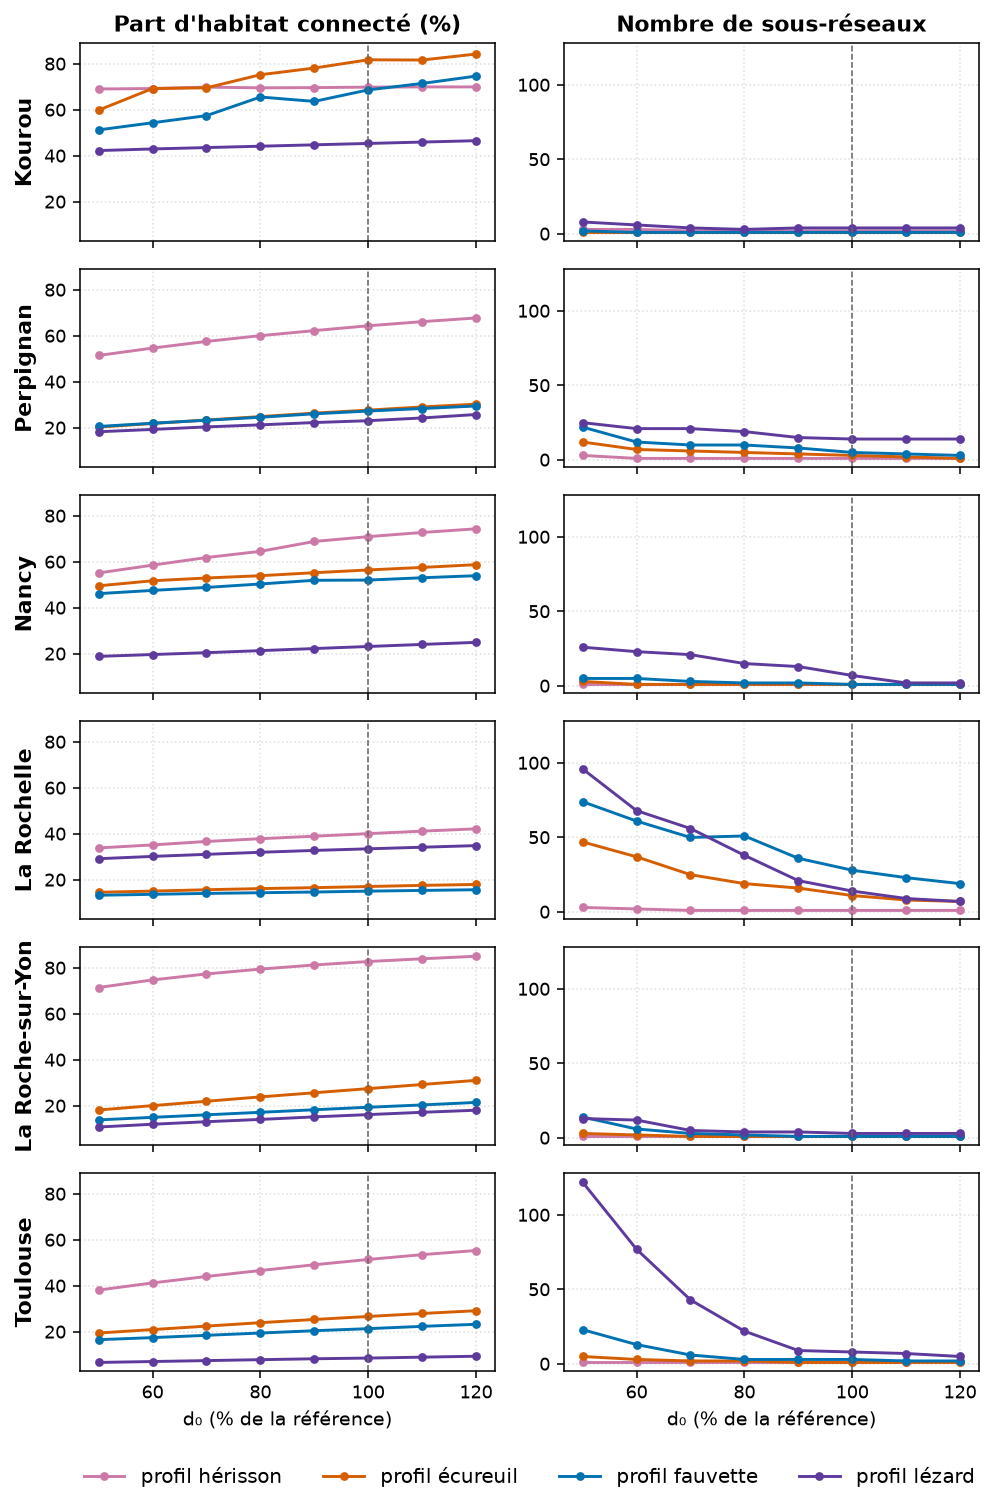
\includegraphics[height=0.86\textheight]{figures/sens_curves_d0.png}
\caption{Courbes de réponse à la distance de dispersion, de 50 à 120 \% de la référence. Un territoire par ligne, un indicateur par colonne, une couleur par profil écologique.}
\label{fig:sens-d0}
\end{figure}

\section*{Annexe 6. Réponse au contraste de friction}
\phantomsection
\addcontentsline{toc}{section}{Annexe 6. Réponse au contraste de friction}

\begin{figure}[H]
\centering
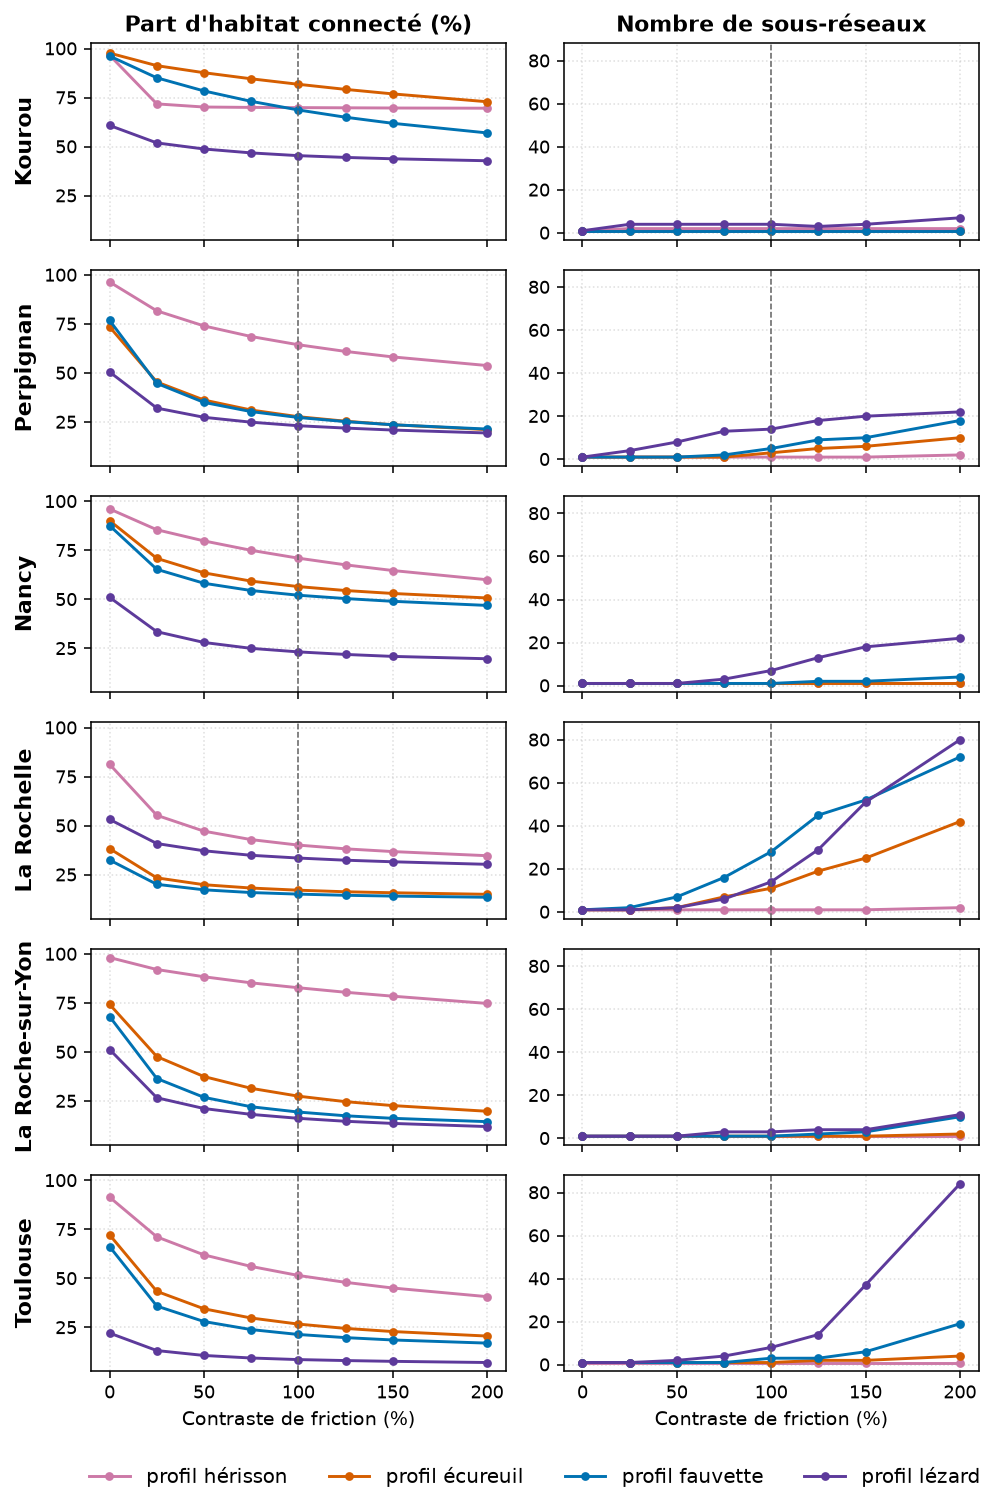
\includegraphics[height=0.86\textheight]{figures/sens_curves_contrast.png}
\caption{Courbes de réponse au contraste de friction, de 0 à 200 \% de la référence. Un territoire par ligne, un indicateur par colonne, une couleur par profil écologique.}
\label{fig:sens-contraste}
\end{figure}

\section*{Annexe 7. Synthèse de sensibilité par territoire et par profil}
\phantomsection
\addcontentsline{toc}{section}{Annexe 7. Synthèse de sensibilité par territoire et par profil}

\begin{table}[H]
\centering
\footnotesize
\setlength{\tabcolsep}{4pt}
\renewcommand{\arraystretch}{1.05}
\caption{Synthèse de sensibilité par territoire et par profil écologique : valeur de référence, puis plage parcourue sur le balayage de la distance de dispersion ($d_0$) et sur celui du contraste de friction.}
\begin{tabular}{@{}llrrrrrr@{}}
\toprule
 & & \multicolumn{3}{c}{\textbf{Part d'habitat connecté}} & \multicolumn{3}{c}{\textbf{Sous-réseaux}} \\
\cmidrule(lr){3-5} \cmidrule(lr){6-8}
\textbf{Territoire} & \textbf{Profil} & \textbf{réf.} & \textbf{$d_0$} & \textbf{contraste} & \textbf{réf.} & \textbf{$d_0$} & \textbf{contraste} \\
\midrule
Kourou & Hérisson & 70 \% & 69 à 70 \% & 70 à 97 \% & 2 & 2 à 3 & 1 à 2 \\
Kourou & Écureuil & 82 \% & 60 à 84 \% & 73 à 98 \% & 1 & 1 & 1 \\
Kourou & Fauvette & 69 \% & 51 à 75 \% & 57 à 96 \% & 1 & 1 à 2 & 1 \\
Kourou & Lézard & 45 \% & 42 à 47 \% & 43 à 61 \% & 4 & 3 à 8 & 1 à 7 \\
Perpignan & Hérisson & 64 \% & 52 à 68 \% & 54 à 96 \% & 1 & 1 à 3 & 1 à 2 \\
Perpignan & Écureuil & 28 \% & 20 à 30 \% & 21 à 74 \% & 3 & 1 à 12 & 1 à 10 \\
Perpignan & Fauvette & 27 \% & 21 à 30 \% & 21 à 77 \% & 5 & 3 à 22 & 1 à 18 \\
Perpignan & Lézard & 23 \% & 18 à 26 \% & 19 à 50 \% & 14 & 14 à 25 & 1 à 22 \\
Nancy & Hérisson & 71 \% & 55 à 74 \% & 60 à 96 \% & 1 & 1 & 1 \\
Nancy & Écureuil & 56 \% & 50 à 59 \% & 51 à 90 \% & 1 & 1 à 3 & 1 \\
Nancy & Fauvette & 52 \% & 46 à 54 \% & 47 à 88 \% & 1 & 1 à 5 & 1 à 4 \\
Nancy & Lézard & 23 \% & 19 à 25 \% & 20 à 51 \% & 7 & 2 à 26 & 1 à 22 \\
La Rochelle & Hérisson & 40 \% & 34 à 42 \% & 35 à 81 \% & 1 & 1 à 3 & 1 à 2 \\
La Rochelle & Écureuil & 17 \% & 15 à 18 \% & 15 à 38 \% & 11 & 7 à 47 & 1 à 42 \\
La Rochelle & Fauvette & 15 \% & 13 à 16 \% & 14 à 32 \% & 28 & 19 à 74 & 1 à 72 \\
La Rochelle & Lézard & 34 \% & 29 à 35 \% & 30 à 53 \% & 14 & 7 à 96 & 1 à 80 \\
La Roche-sur-Yon & Hérisson & 83 \% & 72 à 85 \% & 75 à 98 \% & 1 & 1 & 1 \\
La Roche-sur-Yon & Écureuil & 28 \% & 18 à 31 \% & 20 à 74 \% & 1 & 1 à 3 & 1 à 2 \\
La Roche-sur-Yon & Fauvette & 19 \% & 14 à 22 \% & 14 à 68 \% & 1 & 1 à 14 & 1 à 10 \\
La Roche-sur-Yon & Lézard & 16 \% & 11 à 18 \% & 12 à 51 \% & 3 & 3 à 13 & 1 à 11 \\
Toulouse & Hérisson & 52 \% & 38 à 55 \% & 41 à 91 \% & 1 & 1 & 1 \\
Toulouse & Écureuil & 27 \% & 20 à 28 \% & 21 à 72 \% & 1 & 1 à 5 & 1 à 4 \\
Toulouse & Fauvette & 21 \% & 17 à 23 \% & 17 à 66 \% & 3 & 2 à 23 & 1 à 19 \\
Toulouse & Lézard & 9 \% & 7 à 9 \% & 7 à 22 \% & 8 & 5 à 122 & 1 à 84 \\
\bottomrule
\end{tabular}
\end{table}

\section*{Annexe 8. Espèces retenues et effectifs d'occurrences GBIF}
\phantomsection
\addcontentsline{toc}{section}{Annexe 8. Espèces retenues et effectifs d'occurrences GBIF}

Chaque profil écologique est représenté par un groupe de quatre espèces communes en France métropolitaine : le profil hérisson par le hérisson d'Europe (\textit{Erinaceus europaeus}), la musaraigne pygmée (\textit{Sorex minutus}), le mulot sylvestre (\textit{Apodemus sylvaticus}) et la belette d'Europe (\textit{Mustela nivalis}) ; le profil écureuil par l'écureuil roux (\textit{Sciurus vulgaris}), le loir gris (\textit{Glis glis}), le muscardin (\textit{Muscardinus avellanarius}) et le lérot (\textit{Eliomys quercinus}) ; le profil fauvette par la fauvette à tête noire (\textit{Sylvia atricapilla}), le rougegorge familier (\textit{Erithacus rubecula}), la fauvette grisette (\textit{Sylvia communis}) et la grive musicienne (\textit{Turdus philomelos}) ; le profil lézard par le lézard des murailles (\textit{Podarcis muralis}), l'orvet fragile (\textit{Anguis fragilis}), la couleuvre d'Esculape (\textit{Zamenis longissimus}) et le lézard à deux raies (\textit{Lacerta bilineata}).

\begin{table}[H]
\centering
\small
\caption{Effectifs d'occurrences focales GBIF par profil écologique et par territoire. (d'après les données GBIF, 2026)}
\begin{tabularx}{\linewidth}{>{\raggedright\arraybackslash}X >{\raggedright\arraybackslash}X >{\raggedright\arraybackslash}X >{\raggedright\arraybackslash}X >{\raggedright\arraybackslash}X >{\raggedright\arraybackslash}X >{\raggedright\arraybackslash}X}
\toprule
\textbf{Profil écologique} & \textbf{Perpignan} & \textbf{Toulouse} & \textbf{Nancy} & \textbf{La Roche-sur-Yon} & \textbf{La Rochelle} & \textbf{Total} \\
\midrule
Profil hérisson & 4* & 64 & 3* & 9* & 9* & 89 \\
Profil écureuil & 15* & 129 & 39 & 6* & 4* & 193 \\
Profil fauvette & 126 & 710 & 29* & 40 & 89 & 994 \\
Profil lézard & 1* & 222 & 19* & 26* & 23* & 291 \\
\bottomrule
\end{tabularx}

{\small * effectif inférieur à trente occurrences, couple non interprétable isolément.}
\end{table}

\section*{Annexe 9. Ratios de sélection GBIF}
\phantomsection
\addcontentsline{toc}{section}{Annexe 9. Ratios de sélection GBIF}

\begin{table}[H]
\centering
\small
\caption{Ratios de sélection GBIF par profil écologique et par couche, agrégés sur les cinq territoires métropolitains, avec intervalle de confiance à 95 \% (bootstrap, 1 000 tirages). (d'après les données GBIF, 2026)}
\begin{tabularx}{\textwidth}{>{\raggedright\arraybackslash}X >{\raggedright\arraybackslash}X >{\raggedright\arraybackslash}X >{\raggedright\arraybackslash}X >{\raggedright\arraybackslash}X}
\toprule
\textbf{Profil écologique (n)} & \textbf{Noyau} & \textbf{Espace relais} & \textbf{Tracé} & \textbf{Matrice} \\
\midrule
Profil hérisson (89) & 0,39 [0,23 à 0,57] & 1,92 [0,96 à 3,04] & 1,74 [1,06 à 2,42] & 1,45 [1,14 à 1,80] \\
Profil écureuil (193) & 1,68 [1,48 à 1,88] & 1,18 [0,68 à 1,67] & 0,64 [0,34 à 0,94] & 0,50 [0,38 à 0,63] \\
Profil fauvette (994) & 1,80 [1,65 à 1,95] & 1,65 [1,38 à 1,94] & 0,76 [0,62 à 0,92] & 0,69 [0,64 à 0,74] \\
Profil lézard (291) & 0,86 [0,49 à 1,30] & 0,50 [0,17 à 0,92] & 1,19 [0,89 à 1,48] & 1,00 [0,94 à 1,07] \\
\bottomrule
\end{tabularx}
\end{table}

\section*{Annexe 10. Test du khi-deux sur la répartition des occurrences}
\phantomsection
\addcontentsline{toc}{section}{Annexe 10. Test du khi-deux sur la répartition des occurrences}

\begin{table}[H]
\centering
\small
\caption{Test du khi-deux sur la répartition des occurrences par couche, par profil écologique.}
\begin{tabularx}{\textwidth}{>{\raggedright\arraybackslash}X >{\raggedright\arraybackslash}X >{\raggedright\arraybackslash}X >{\raggedright\arraybackslash}X >{\raggedright\arraybackslash}X}
\toprule
\textbf{Profil} & \textbf{Occurrences} & \textbf{khi-deux (3 ddl)} & \textbf{p} & \textbf{Sélection} \\
\midrule
Fauvette à tête noire & 994 & 166,2 & inférieur à 0,001 & significative \\
Écureuil roux & 193 & 44,1 & inférieur à 0,001 & significative \\
Hérisson d'Europe & 89 & 29,5 & inférieur à 0,001 & significative \\
Lézard des murailles & 291 & 4,5 & 0,21 & non significative \\
\bottomrule
\end{tabularx}
\end{table}

\section*{Annexe 11. Indicateurs de connectivité par territoire et par profil}
\phantomsection
\addcontentsline{toc}{section}{Annexe 11. Indicateurs de connectivité par territoire et par profil}

\begin{table}[H]
\centering
\scriptsize
\setlength{\tabcolsep}{3pt}
\renewcommand{\arraystretch}{1.05}
\caption{Indicateurs de connectivité par territoire et par profil écologique : part d'habitat connecté, nombre de sous-réseaux, surface équivalente connectée, tortuosité médiane, puis dénombrements des composantes. Noyaux et espaces relais comptés dans la zone d'étude stricte, tracés aboutis et liens en échec dès qu'ils la touchent.}
\begin{tabular}{@{}llrrrrrrrr@{}}
\toprule
 & & \multicolumn{4}{c}{\textbf{Indicateurs}} & \multicolumn{4}{c}{\textbf{Dénombrements}} \\
\cmidrule(lr){3-6} \cmidrule(lr){7-10}
\textbf{Territoire} & \textbf{Profil} & \textbf{connecté} & \textbf{sous-rés.} & \textbf{EC (ha)} & \textbf{tortuosité} & \textbf{noyaux} & \textbf{relais} & \textbf{tracés} & \textbf{échecs} \\
\midrule
La Roche-sur-Yon & Hérisson & 83 \% & 1 & 20 864 & 1,66 & 524 & 1515 & 4537 & 1 \\
 & Écureuil & 28 \% & 1 & 2 747 & 1,38 & 591 & 3872 & 9586 & 35 \\
 & Fauvette & 19 \% & 1 & 1 932 & 1,27 & 591 & 3872 & 9414 & 177 \\
 & Lézard & 16 \% & 3 & 2 321 & 1,41 & 1115 & 3350 & 9349 & 520 \\
Nancy & Hérisson & 71 \% & 1 & 4 916 & 1,60 & 159 & 1004 & 2631 & 6 \\
 & Écureuil & 56 \% & 1 & 2 676 & 1,47 & 121 & 1068 & 2566 & 8 \\
 & Fauvette & 52 \% & 1 & 2 468 & 1,41 & 121 & 1068 & 2506 & 65 \\
 & Lézard & 23 \% & 7 & 479 & 1,41 & 127 & 666 & 1334 & 282 \\
Perpignan & Hérisson & 64 \% & 1 & 1 707 & 1,61 & 119 & 391 & 1075 & 7 \\
 & Écureuil & 28 \% & 3 & 209 & 1,37 & 72 & 503 & 1127 & 81 \\
 & Fauvette & 27 \% & 5 & 389 & 1,41 & 110 & 572 & 1281 & 145 \\
 & Lézard & 23 \% & 14 & 270 & 1,41 & 91 & 514 & 1088 & 270 \\
Kourou & Hérisson & 70 \% & 2 & 4 516 & 1,41 & 25 & 125 & 278 & 37 \\
 & Écureuil & 82 \% & 1 & 3 733 & 1,21 & 50 & 150 & 411 & 10 \\
 & Fauvette & 69 \% & 1 & 3 134 & 1,14 & 51 & 150 & 387 & 37 \\
 & Lézard & 45 \% & 4 & 852 & 1,41 & 65 & 221 & 478 & 61 \\
Toulouse & Hérisson & 52 \% & 1 & 7 674 & 1,62 & 570 & 4109 & 10362 & 7 \\
 & Écureuil & 27 \% & 1 & 2 445 & 1,50 & 404 & 4277 & 9930 & 89 \\
 & Fauvette & 21 \% & 3 & 1 965 & 1,41 & 404 & 4277 & 9652 & 348 \\
 & Lézard & 9 \% & 8 & 442 & 1,39 & 467 & 2938 & 6150 & 1004 \\
La Rochelle & Hérisson & 40 \% & 1 & 2 632 & 1,44 & 301 & 1821 & 4371 & 18 \\
 & Écureuil & 17 \% & 11 & 253 & 1,31 & 124 & 891 & 1633 & 253 \\
 & Fauvette & 15 \% & 28 & 223 & 1,24 & 124 & 891 & 1413 & 466 \\
 & Lézard & 34 \% & 14 & 1 627 & 1,47 & 216 & 1954 & 3566 & 807 \\
\bottomrule
\end{tabular}
\end{table}


\clearpage
% Page tournée aux marges réduites : dans une page paysage la hauteur utile est le
% petit côté de la feuille, et cette page porte un export A4 paysage entier. Pas de
% légende de figure, la feuille porte la sienne.
\newgeometry{margin=1cm}
\begin{landscape}
% titre compact et non \section* : sur une page tournée la hauteur utile est le petit
% côté de la feuille, chaque millimètre de titre est pris sur l'image
{\large\bfseries Annexe 12. Planning du stage, prévisionnel et réalisé\par}
\phantomsection
\addcontentsline{toc}{section}{Annexe 12. Planning du stage, prévisionnel et réalisé}
\vspace{2mm}

\centerline{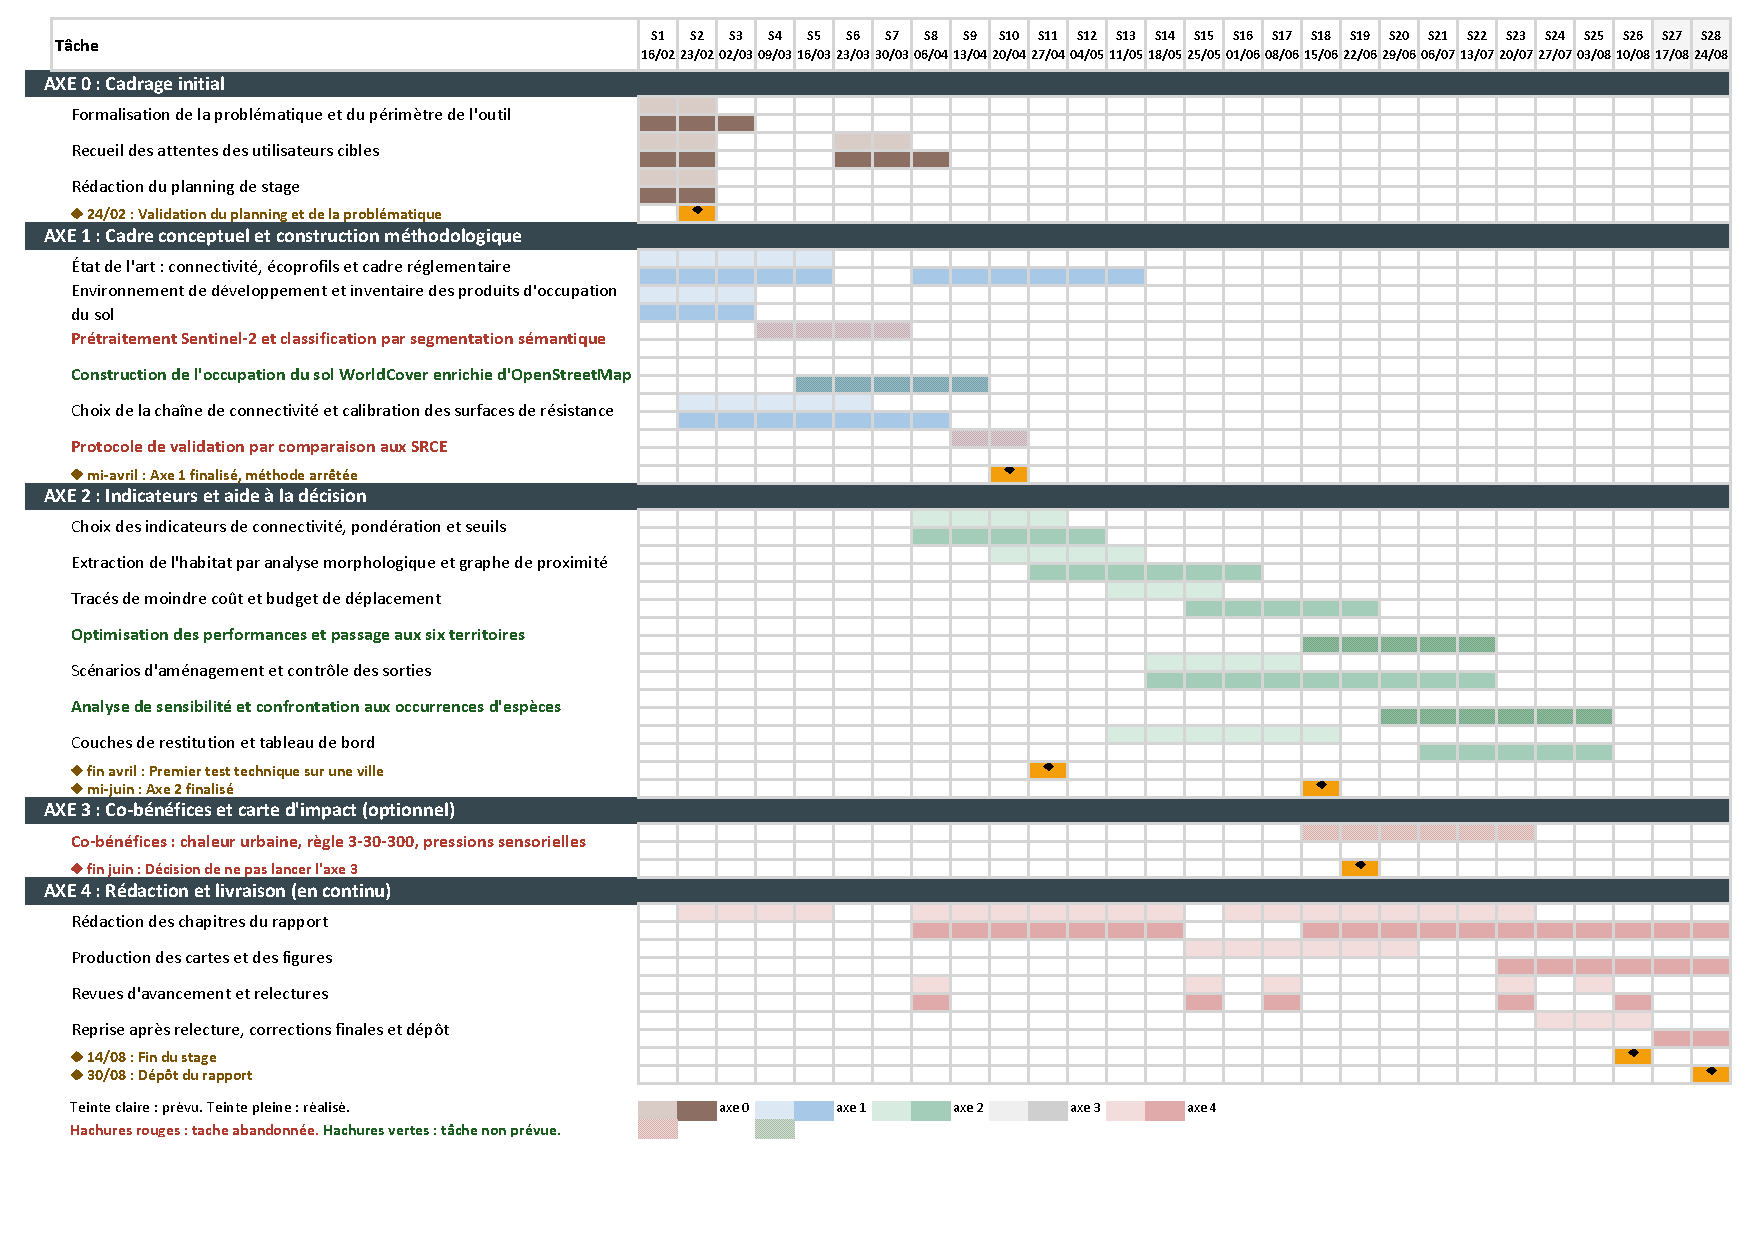
\includegraphics[height=17.8cm]{figures/planning_gantt.pdf}}
\end{landscape}
\restoregeometry

\clearpage
\etocsetnexttocdepth{subsubsection}
\tableofcontents
\listoffigures
\listoftables
\clearpage
{\noindent\Large\bfseries Liste des équations}\par\medskip
\begin{tabular}{@{}ll@{}}
(1) & Probabilité de déplacement entre deux taches ($p_{ij}$)\\
(2) & Probability of Connectivity (PC)\\
(3) & Surface équivalente connectée (EC)\\
\end{tabular}

\end{document}
